% Options for packages loaded elsewhere
\PassOptionsToPackage{unicode}{hyperref}
\PassOptionsToPackage{hyphens}{url}
\PassOptionsToPackage{dvipsnames,svgnames*,x11names*}{xcolor}
%
\documentclass[
  12pt,
]{book}
\usepackage{amsmath,amssymb}
\usepackage{lmodern}
\usepackage{setspace}
\usepackage{ifxetex,ifluatex}
\ifnum 0\ifxetex 1\fi\ifluatex 1\fi=0 % if pdftex
  \usepackage[T1]{fontenc}
  \usepackage[utf8]{inputenc}
  \usepackage{textcomp} % provide euro and other symbols
\else % if luatex or xetex
  \usepackage{unicode-math}
  \defaultfontfeatures{Scale=MatchLowercase}
  \defaultfontfeatures[\rmfamily]{Ligatures=TeX,Scale=1}
\fi
% Use upquote if available, for straight quotes in verbatim environments
\IfFileExists{upquote.sty}{\usepackage{upquote}}{}
\IfFileExists{microtype.sty}{% use microtype if available
  \usepackage[]{microtype}
  \UseMicrotypeSet[protrusion]{basicmath} % disable protrusion for tt fonts
}{}
\makeatletter
\@ifundefined{KOMAClassName}{% if non-KOMA class
  \IfFileExists{parskip.sty}{%
    \usepackage{parskip}
  }{% else
    \setlength{\parindent}{0pt}
    \setlength{\parskip}{6pt plus 2pt minus 1pt}}
}{% if KOMA class
  \KOMAoptions{parskip=half}}
\makeatother
\usepackage{xcolor}
\IfFileExists{xurl.sty}{\usepackage{xurl}}{} % add URL line breaks if available
\IfFileExists{bookmark.sty}{\usepackage{bookmark}}{\usepackage{hyperref}}
\hypersetup{
  pdftitle={Conceptual and methodological problems with bias detection and avoidance in natural language processing},
  pdfauthor={Alicja Dobrzeniecka},
  colorlinks=true,
  linkcolor=Maroon,
  filecolor=Maroon,
  citecolor=Blue,
  urlcolor=blue,
  pdfcreator={LaTeX via pandoc}}
\urlstyle{same} % disable monospaced font for URLs
\usepackage[left=3.5cm, right=2.5cm, top=2.5cm, bottom=2.5cm, asymmetric, includeheadfoot]{geometry}
\usepackage{color}
\usepackage{fancyvrb}
\newcommand{\VerbBar}{|}
\newcommand{\VERB}{\Verb[commandchars=\\\{\}]}
\DefineVerbatimEnvironment{Highlighting}{Verbatim}{commandchars=\\\{\}}
% Add ',fontsize=\small' for more characters per line
\usepackage{framed}
\definecolor{shadecolor}{RGB}{248,248,248}
\newenvironment{Shaded}{\begin{snugshade}}{\end{snugshade}}
\newcommand{\AlertTok}[1]{\textcolor[rgb]{0.94,0.16,0.16}{#1}}
\newcommand{\AnnotationTok}[1]{\textcolor[rgb]{0.56,0.35,0.01}{\textbf{\textit{#1}}}}
\newcommand{\AttributeTok}[1]{\textcolor[rgb]{0.77,0.63,0.00}{#1}}
\newcommand{\BaseNTok}[1]{\textcolor[rgb]{0.00,0.00,0.81}{#1}}
\newcommand{\BuiltInTok}[1]{#1}
\newcommand{\CharTok}[1]{\textcolor[rgb]{0.31,0.60,0.02}{#1}}
\newcommand{\CommentTok}[1]{\textcolor[rgb]{0.56,0.35,0.01}{\textit{#1}}}
\newcommand{\CommentVarTok}[1]{\textcolor[rgb]{0.56,0.35,0.01}{\textbf{\textit{#1}}}}
\newcommand{\ConstantTok}[1]{\textcolor[rgb]{0.00,0.00,0.00}{#1}}
\newcommand{\ControlFlowTok}[1]{\textcolor[rgb]{0.13,0.29,0.53}{\textbf{#1}}}
\newcommand{\DataTypeTok}[1]{\textcolor[rgb]{0.13,0.29,0.53}{#1}}
\newcommand{\DecValTok}[1]{\textcolor[rgb]{0.00,0.00,0.81}{#1}}
\newcommand{\DocumentationTok}[1]{\textcolor[rgb]{0.56,0.35,0.01}{\textbf{\textit{#1}}}}
\newcommand{\ErrorTok}[1]{\textcolor[rgb]{0.64,0.00,0.00}{\textbf{#1}}}
\newcommand{\ExtensionTok}[1]{#1}
\newcommand{\FloatTok}[1]{\textcolor[rgb]{0.00,0.00,0.81}{#1}}
\newcommand{\FunctionTok}[1]{\textcolor[rgb]{0.00,0.00,0.00}{#1}}
\newcommand{\ImportTok}[1]{#1}
\newcommand{\InformationTok}[1]{\textcolor[rgb]{0.56,0.35,0.01}{\textbf{\textit{#1}}}}
\newcommand{\KeywordTok}[1]{\textcolor[rgb]{0.13,0.29,0.53}{\textbf{#1}}}
\newcommand{\NormalTok}[1]{#1}
\newcommand{\OperatorTok}[1]{\textcolor[rgb]{0.81,0.36,0.00}{\textbf{#1}}}
\newcommand{\OtherTok}[1]{\textcolor[rgb]{0.56,0.35,0.01}{#1}}
\newcommand{\PreprocessorTok}[1]{\textcolor[rgb]{0.56,0.35,0.01}{\textit{#1}}}
\newcommand{\RegionMarkerTok}[1]{#1}
\newcommand{\SpecialCharTok}[1]{\textcolor[rgb]{0.00,0.00,0.00}{#1}}
\newcommand{\SpecialStringTok}[1]{\textcolor[rgb]{0.31,0.60,0.02}{#1}}
\newcommand{\StringTok}[1]{\textcolor[rgb]{0.31,0.60,0.02}{#1}}
\newcommand{\VariableTok}[1]{\textcolor[rgb]{0.00,0.00,0.00}{#1}}
\newcommand{\VerbatimStringTok}[1]{\textcolor[rgb]{0.31,0.60,0.02}{#1}}
\newcommand{\WarningTok}[1]{\textcolor[rgb]{0.56,0.35,0.01}{\textbf{\textit{#1}}}}
\usepackage{longtable,booktabs,array}
\usepackage{calc} % for calculating minipage widths
% Correct order of tables after \paragraph or \subparagraph
\usepackage{etoolbox}
\makeatletter
\patchcmd\longtable{\par}{\if@noskipsec\mbox{}\fi\par}{}{}
\makeatother
% Allow footnotes in longtable head/foot
\IfFileExists{footnotehyper.sty}{\usepackage{footnotehyper}}{\usepackage{footnote}}
\makesavenoteenv{longtable}
\usepackage{graphicx}
\makeatletter
\def\maxwidth{\ifdim\Gin@nat@width>\linewidth\linewidth\else\Gin@nat@width\fi}
\def\maxheight{\ifdim\Gin@nat@height>\textheight\textheight\else\Gin@nat@height\fi}
\makeatother
% Scale images if necessary, so that they will not overflow the page
% margins by default, and it is still possible to overwrite the defaults
% using explicit options in \includegraphics[width, height, ...]{}
\setkeys{Gin}{width=\maxwidth,height=\maxheight,keepaspectratio}
% Set default figure placement to htbp
\makeatletter
\def\fps@figure{htbp}
\makeatother
\setlength{\emergencystretch}{3em} % prevent overfull lines
\providecommand{\tightlist}{%
  \setlength{\itemsep}{0pt}\setlength{\parskip}{0pt}}
\setcounter{secnumdepth}{5}
\usepackage{todonotes}
\ifluatex
  \usepackage{selnolig}  % disable illegal ligatures
\fi
\newlength{\cslhangindent}
\setlength{\cslhangindent}{1.5em}
\newlength{\csllabelwidth}
\setlength{\csllabelwidth}{3em}
\newenvironment{CSLReferences}[2] % #1 hanging-ident, #2 entry spacing
 {% don't indent paragraphs
  \setlength{\parindent}{0pt}
  % turn on hanging indent if param 1 is 1
  \ifodd #1 \everypar{\setlength{\hangindent}{\cslhangindent}}\ignorespaces\fi
  % set entry spacing
  \ifnum #2 > 0
  \setlength{\parskip}{#2\baselineskip}
  \fi
 }%
 {}
\usepackage{calc}
\newcommand{\CSLBlock}[1]{#1\hfill\break}
\newcommand{\CSLLeftMargin}[1]{\parbox[t]{\csllabelwidth}{#1}}
\newcommand{\CSLRightInline}[1]{\parbox[t]{\linewidth - \csllabelwidth}{#1}\break}
\newcommand{\CSLIndent}[1]{\hspace{\cslhangindent}#1}

\title{Conceptual and methodological problems with bias detection and avoidance in natural language processing}
\author{Alicja Dobrzeniecka}
\date{2021-06-23}

\begin{document}
\maketitle

{
\hypersetup{linkcolor=}
\setcounter{tocdepth}{5}
\tableofcontents
}
\setstretch{1.5}
\hypertarget{introduction}{%
\chapter{Introduction}\label{introduction}}

Natural language processing (NLP) is a subfield of computer science that processes and analyzes language in text and speech with the use of modern programming methods. It has practical applications in everyday life as it concerns tasks such as email filters, smart assistants, search results, language translations, text analytics and so on. Models used to accomplish these tasks need a lot of data to learn from. This data originates from human activities and historical recordings such as texts, messages or speeches. It turns out that in the learning process these models can learn implicit biases that reflect harmful stereotypical thinking still present in modern societies. There are many different types of models in NLP depending on a task that they are supposed to solve. However, all of them need as an input words represented by means of numbers and this is accomplished with word embeddings. Word embeddings are usually assigned the values based on the context in which the words appear. This means that the input data can have an enormous influence on the outcome. One can find methods that aim at identifying and measuring hidden biases and/or try to remove them by, for example, modifying the word embeddings directly.

One can find various definitions trying to capture what bias and fairness actually are. With the choice of the definition, implications for the real-life applications may change as well. \protect\hyperlink{ref-Mehrabi2019Survey}{Mehrabi, Morstatter, Saxena, Lerman, \& Galstyan} (\protect\hyperlink{ref-Mehrabi2019Survey}{2019}) mark out that there exist different types of biases such as historical bias, representation bias or measurement bias (the list is long). This indicates how complex the issue of bias is. Without the proper understanding and awareness of the problem, people are prone to unconsciously sustain the bias. \protect\hyperlink{ref-Mehrabi2019Survey}{Mehrabi, Morstatter, Saxena, Lerman, \& Galstyan} (\protect\hyperlink{ref-Mehrabi2019Survey}{2019}) also distinguish different types of discrimination, some of them will be briefly described. By protected attributes we mean those qualities, traits or characteristics that one should not discriminate against. Direct discrimination occurs when protected attributes of individuals explicitly result in non-favorable outcomes toward them. Such discrimination takes place for example when one uses the information about someone's religious beliefs to evaluate whether they are competent for the work they apply for. In contrast, in indirect discrimination individuals appear to be treated equally, but anyway they end up being treated unjustly due to the hidden effects of biases towards their protected attributes. An example of such situation is when in a job advert there is a requirement of 10 years experience instead of the list of a specific type of experience and knowledge. This job advert can discriminate indirectly against young people who can have the required skills, but not yet so much work experience. Systemic discrimination takes place when policies, customs or behaviors that result from certain culture or organizational structure lead to discrimination against some groups of people. Finally, statistical discrimination consists in relying on group statistics to judge a person belonging to a given group. The topic of discrimination is entangled with another concept; fairness. It is essential to grasp some concepts of fairness to take them into consideration while designing implementation of some machine learning model. In \protect\hyperlink{ref-Mehrabi2019Survey}{Mehrabi, Morstatter, Saxena, Lerman, \& Galstyan} (\protect\hyperlink{ref-Mehrabi2019Survey}{2019}) one may notice that depending on the context and application different definitions may be applied.

There is a considerable amount of literature available on the topic of bias detection and mitigation in NLP models. \protect\hyperlink{ref-Bolukbasi2016Man}{Bolukbasi, Chang, Zou, Saligrama, \& Kalai} (\protect\hyperlink{ref-Bolukbasi2016Man}{2016}) focus on gender biases that may be observable in the representation of job occupations and gender in terms of numerical
values. The authors apply cosine similarity measurement to investigate the phenomenon where (the vectors corresponding to) words related to jobs that are stereotypically associated with a given gender are in fact in the model situated closer to this gender.
They also use analogy tasks to evaluate if a bias is present in a word embedding model. They check analogies by comparing pairs of word vectors. For example they search for the word complementing the puzzle: man is to doctor as woman is to \ldots? First they subtract the word ``man'' from the word ``woman''\footnote{This is pointwise subtraction of vectors, but for the simplicity we will often talk about words while really meaning vectors. What is meant should be clear from the context.} and then
they search for the ranked list of other words pairs that have similar vector difference. They also include in the formula a threshold to ensure that the resulting pairs could not be randomly picked.

However, as \protect\hyperlink{ref-Nissim2019Fair}{Nissim, Noord, \& Goot} (\protect\hyperlink{ref-Nissim2019Fair}{2019}) points out, there are some limitations to this approach. In practice, most of analogies implementations do not return any input words. This means that it does not make sense to expect the algorithm to return the same profession for both woman and man. Therefore, this method of bias detection seems limited. Other problems are related for example to the choice of pairs and words that are used to detect the presence of discrimination, as it is often subjective and without proper justification. Additionally, the choice of the parameter used in \protect\hyperlink{ref-Bolukbasi2016Man}{Bolukbasi, Chang, Zou, Saligrama, \& Kalai} (\protect\hyperlink{ref-Bolukbasi2016Man}{2016}) formula to ensure that word pairs are not picked by random, is also not justified and changing it drastically
influences the results.

\protect\hyperlink{ref-Caliskan2017Semantics}{Islam, Bryson, \& Narayanan} (\protect\hyperlink{ref-Caliskan2017Semantics}{2016}) touch upon the topic of biases regarding race and gender. They apply knowledge from well-known psychological studies such as Implicit Association Test to investigate the relation between human stereotypical thinking and model-learnt biases to discover a close relationship between these two. For the evaluation they use Word Embedding Association Test (WEAT) and the Word Embedding Factual Association Test (WEFAT).

\protect\hyperlink{ref-Manzini2019blackToCriminal}{Manzini, Lim, Tsvetkov, \& Black} (\protect\hyperlink{ref-Manzini2019blackToCriminal}{2019}) propose a novel way of using cosine similarity to verify if the assumed resemblance between protected words and harmful attributes exists. They develop an approach that enables them to measure the bias for a class (such as gender, religion or race) and express the final result with a single metric. Their approach will be analyzed in details in the next chapter.

\protect\hyperlink{ref-Caliskan2017Semantics}{Islam, Bryson, \& Narayanan} (\protect\hyperlink{ref-Caliskan2017Semantics}{2016}) refer to Implicit Association Test (Greenwald et al., 1998) that measures the strength of associations between concepts or stereotypes by measuring human reaction time for special tasks. Humans naturally exhibit some biases which do not always cause social concern. One can imagine the intuitive associations between for example insects and flowers, and the feelings of pleasantness or unpleasantness. In general, people would rather associate flowers than insects with feeling pleasant, and this preference in a sense is a bias or
prejudice in some direction. However, this type of preference does not cause an uproar and is a rather morally neutral case. This example is rather used to show that the methodology used in IAT makes sense. \protect\hyperlink{ref-Caliskan2017Semantics}{Islam, Bryson, \& Narayanan} (\protect\hyperlink{ref-Caliskan2017Semantics}{2016}) were able to obtain similar results to the ones that measured reaction time with the use of WEAT metric. Unfortunately, further studies discover other biases and prejudices that directly influence the quality of other people's lives and therefore they should be taken care of.

The most common bias detection methods in the literature focus on comparing the similarity between words from protected groups and those that are considered to be stereotypical or harmful in some way. One can find in this group methods such as Euclidean distance or cosine similarity (which is equivalent to dot product if the vectors are normalized). There are also other ways to detect the effects of biases. One can investigate the model performance on certain downstream tasks and validate if the model uses the gender or race information to complete the task. Unfortunately, the currently used methods employing cosine similarity, often aggregate the similarity values in a way that may lead to hasty conclusions. The averaging of values and the lack of attention to uncertainty involved in such aggregation may lead to an incomplete picture of the situation.

In the paper we indicate how current methods used to detect biases in natural language models are limited, if we investigate them from the perspective of Bayesian analysis. Our research enhances the current way in which the bias detection is performed to make sure that it is methodologically valid. The key hypothesis is that greater understanding of data and bias implications can be achieved when Bayesian methods are applied to issue.

\hypertarget{cosine-similarity-and-bias-detection}{%
\chapter{Cosine similarity and bias detection}\label{cosine-similarity-and-bias-detection}}

\hypertarget{word-embeddings}{%
\section{Word embeddings}\label{word-embeddings}}

To understand what cosine similarity measurement is, one first needs to grasp the concept of translating words to a computer-readable form. In the field of natural language processsing there are two main types of words representation --- localist and distributed. One-hot encoding is an example of a method used to achieve a localist representation of words. Here, each vector contains information only about a single data point. This is achieved by first mapping categorical values (words) to integers and then to each integers a binary vector is assigned which contains only 0s except for the index of the integer, which is assigned 1. An example of a localist representation is:

\begin{longtable}[]{@{}llllll@{}}
\toprule
word & 1 & 2 & 3 & 4 & 5 \\
\midrule
\endhead
woman & 1 & 0 & 0 & 0 & 0 \\
man & 0 & 1 & 0 & 0 & 0 \\
girl & 0 & 0 & 1 & 0 & 0 \\
boy & 0 & 0 & 0 & 1 & 0 \\
monarch & 0 & 0 & 0 & 0 & 1 \\
\bottomrule
\end{longtable}

In the example above it is clear that the length of the vectors increases with the number of words in a vocabulary. It is not a very computationally efficient representation. It has other flaws as well. For example, it is unable to capture the resemblance between words appearing in similar contexts.

In contrast to the localist representation, a distributed representation returns vectors that contain continuous values instead of discrete 1s and 0s. Word embeddings are a class of various techniques that allow one to represent words as distributed vectors. Such learned representations of text have certain properties. At least prima facie, they store similar (or at least co-occurring) words close to each other in a vector space. An example of distributed representation is:

\begin{longtable}[]{@{}lllll@{}}
\toprule
word & 1 & 2 & 3 & 4 \\
\midrule
\endhead
woman & 0.456 & 0.267 & 0.675 & 0.131 \\
man & 0.451 & 0.897 & 0.472 & 0.088 \\
girl & 0.604 & 0.262 & 0.414 & 0.706 \\
boy & 0.279 & 0.172 & 0.475 & 0.010 \\
monarch & 0.565 & 0.678 & 0.463 & 0.975 \\
\bottomrule
\end{longtable}

One of the advantages of using a distributed representation is that one is able to represent an enormous number of concepts with a smaller number of units. It is also possible to better capture similarities as words of similar meanings can have similar numeric vectors.

The numbers occurring in such representations are not random. They are learned in a process that uses a very shallow neural network. There are various types of techniques used for learning the vectors representations. One of the most straightforward ones is a skip-gram model.
Given a word, the model tries to predict its neighboring words from the sentence. The mathematics behind the process relies on the idea that the prediction concerns the conditional probability of the adjacent words. The algorithm tries to minimize the loss function, which penalizes the system for discrepancy with actual co-occurrence frequencies in the corpus. One can choose various parameters of the model, such as the window size that determines how many surrounding words the model should predict. After preparing such a fitted model, one takes only the learned weights from a neural network, and uses them as vectors in a word embeddings representation.

Word embeddings have many applications in natural language processing. They are handy in document search and information retrieval. They also play their part in improving automatic translations. Well learned word representations may also contribute to the improvement of sentiment analysis or spam detection.

\hypertarget{cosine-similarity-and-distance}{%
\section{Cosine similarity and distance}\label{cosine-similarity-and-distance}}

Cosine similarity is often used as a method of finding out whether vector representations for two words suggest that they are similar or somehow connected. Cosine similarity is the cosine of the angle between two vectors: the result of dividing their inner product (dot product usually) by the product of their magnitudes.

It is worth mentioning one more point concerning cosine similarity. After the vectors are normalized to have length equal to 1, the inner product itself (often dot product) is used to measure the similarity, because it then equals the cosine similarity.

\begin{align} \tag{Sim}
\mathsf{cosineSimilarity}(A,B) & = \frac{A \cdot B}{\vert \vert A \vert \vert \,\vert \vert B \vert \vert}
\end{align}
Cosine similarity is considered a proper tool for this operation as its result has a clear connection to geometry and at least for a low number of dimensions may be easily interpreted. Using this scale, one can compare vector similarities in a fairly clear manner. When the vectors are aligned perpendicularly to each other, their similarity equals 0 (which is the same as the cosine of 90 degrees). This tells us that the similarity between the vectors is small. As the angle between vectors decreases, cosine similarity approaches one, which stands for the greatest similarity. It is also possible to obtain negative cosine similarity. If the value approaches -1, this intuitively means that the words are contrary to each other.

One of the limitations of this measure is that it informs us only about similarities between vectors in terms of their orientation. However, it is often argued that in comparing words in terms of this metric, the magnitude of vectors may be treated as irrelevant, as the most important information pertains to direction.

In what follows, it is important to distinguish between cosine similarity and cosine distance, defined as:
\begin{align} \tag{Sim}
\mathsf{cosineDistance}(A,B) &  = 1 - \mathsf{cosineSimilarity}(A,B)\\
 &  = 1 - \frac{A \cdot B}{\vert \vert A \vert \vert \,\vert \vert B \vert \vert} \nonumber
\end{align}

The greater the similarity between two vectors, the smaller the distance between them. The cosine distance ranges between 0 and 2. If the vectors are in an opposite directions, the cosine distance is 2. And if the vectors are extremely similar then the cosine distance is very close to 0.

One should note that cosine distance is not exactly a distance measure, as it does not meet triangle inequality requirements. The triangle inequality formula says that for any triangle, the sum of the lengths of any two sides must be greater than or equal to the length of the remaining side. As shown in \href{https://stats.stackexchange.com/questions/198080/proving-that-cosine-distance-function-defined-by-cosine-similarity-between-two-u}{discussion in stats.stackexchange.com}\footnote{\url{https://stats.stackexchange.com/questions/198080/proving-that-cosine-distance-function-defined-by-cosine-similarity-between-two-u}} in the case of cosine distance it would have to fulfill this equation \(1+\mathsf{cos-sim}(A,C) < \mathsf{cos-sim}(A,B) + \mathsf{cos-sim}(B,C)\). If one chooses specific unit vectors it is easy to demonstrate that the triangle inequality is not preserved.

\hypertarget{cosine-distance-in-a-one-class-bias-detection}{%
\section{Cosine distance in a one-class bias detection}\label{cosine-distance-in-a-one-class-bias-detection}}

\protect\hyperlink{ref-Bolukbasi2016Man}{Bolukbasi, Chang, Zou, Saligrama, \& Kalai} (\protect\hyperlink{ref-Bolukbasi2016Man}{2016}) define similarity between words as the outcome inner product of their normalized vectors.
They focus on examining what the geometry of a word embedding is in regard to ``he'' and ``she'' words. In other words, whether the similarity between those concepts and other words reflects expected gender stereotypes. They test this hypothesis by investigating whether there is a connection between word embeddings representing certain professions and words referring to gender. They also evaluate whether automatically produced analogies between words reflect the stereotypes as well.

Here the gender bias of a word \(w\) is understood as its projection on the gender direction \(\vec{w} \cdot (\overrightarrow{he} - \overrightarrow{she})\) (the gender direction is the top principal compontent of ten gender pair difference vectors). The underlying idea is that no bias is present if non-explicitly gender words are in equal distance to both elements in all explicitly gender pairs. Given the (ideally) gender neutral words \(N\) and the gender direction \(g\) the direct direct gender bias is defined as the average distance of the words in \(N\) from \(g\) (\(c\) is a parameter determining how strict we want to be):
\begin{align}
\mathsf{directBias_c(N,g)} & = \frac{\sum_{w\in N}\vert \mathsf{cos}(\vec{w},g)\vert^c}{\vert N \vert }
\end{align}

A very vivid way to follow their method of arguing that bias in word embeddings is real is to plot the values of inner product of chosen words. The plot below does not originate from the original paper but from \href{https://www.kaggle.com/rtatman/gender-bias-in-word-embeddings}{kaggle.com R notebook using data from GloVe: Global Vectors for Word Representation}.\footnote{\url{https://www.kaggle.com/rtatman/gender-bias-in-word-embeddings}.} However, similar visualization may be found there. Data used to create our plot is as follows.

Occupations associated with feminine: \textbf{"homemaker", "nurse", "receptionist", "librarian", "socialite", "hairdresser", "nanny", "bookkeeper", "stylist", "housekeeper", "interior designer", "guidance counselor"}

Occupations associated with masculine: \textbf{"maestro", "skipper", "protege", "philosopher", "captain", "architect", "financier", "warrior", "broadcaster", "magician", "fighter pilot", "boss"}

\vspace{1mm}
\footnotesize

\begin{center}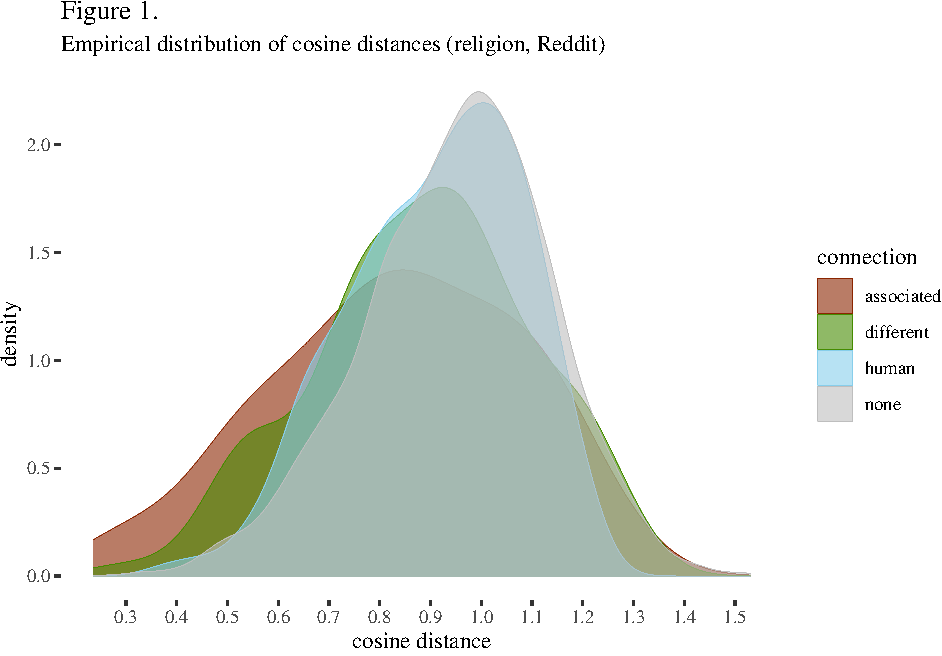
\includegraphics[width=1\linewidth]{_main_files/figure-latex/unnamed-chunk-1-1} \end{center}
\normalsize

The points in the plot above result from the calculation of the inner product of a chosen vector for a profession word and a vector for a gender word (she or he). Inner product of two vectors expresses similarity between words. This assumption originates from the geometry and properties of a vector space. In the picture one may observe a correlation between the occupation and gender. Stereotypical male professions are closer to the ``he'' word and stereotypical female professions have greater similarity with ``she'' word. One could argue that this is a hint that there is some hidden bias information stored in the words vectors.

\hypertarget{cosine-distance-in-a-multi-class-bias-detection}{%
\section{Cosine distance in a multi-class bias detection}\label{cosine-distance-in-a-multi-class-bias-detection}}

\protect\hyperlink{ref-Manzini2019blackToCriminal}{Manzini, Lim, Tsvetkov, \& Black} (\protect\hyperlink{ref-Manzini2019blackToCriminal}{2019}) present a different approach towards finding similarities between classes of words. Cosine distance is used in the article as a measure to first argue for the existence of multi-class bias and then to show how through bias mitigation techniques the bias may be decreased.

They modify WEAT to a multi-class setting, introducing Mean Average Cosine similarity as a measure of bias (in fact, in the paper they report distances rather than similarities). Let \(T = \{t_1, \dots, t_k\}\) be a class of protected word embeddings, and let each \(A_j\in A\) be a set of attributes stereotypically associated with a protected word). Then:
\begin{align}
S(t_i, A_j) & = \frac{1}{\vert A_j\vert}\sum_{a\in A_j}\mathsf{cos}(t,a) \\
MAC(T,A) & = \frac{1}{\vert T \vert \,\vert A\vert}\sum_{t_i \in T }\sum_{A_j \in A} S(t_i,A_j)
\end{align}

As the code has been provided by the authors we were able to reconstruct their results. The main steps in the procedure are as follows. Let us go through an example that refers to the process of hard debiasing on religious attributes.

First we load word embeddings from reddit.US.txt.tok.clean.cleanedforw2v.w2v dataset. The word embeddings have only 50 dimensions and the number of individual words from the dataset is 44895. The authors assume that the protected group should ideally not have high cosine similarity to stereotypical words. The word embeddings geometry should not place this group close to harmful stereotypes, if it is to be bias-free. For instance, let's look at the religion-related words.

Protected words by religion type:

\begin{minipage}{1.0\textwidth}
\textbf{"jew"       : ["judaism", "jew", "synagogue", "torah", "rabbi"]} 

\textbf{"christian" : ["christianity", "christian", "church", "bible", "priest"]}

\textbf{"muslim"    : ["islam", "muslim", "mosque", "quran", "imam"]}
\end{minipage}

Stereotypical words by religion type:

\begin{minipage}{1.0\textwidth}
\textbf{"jew"       : ["greedy", "cheap", "hairy", "liberal"]}

\textbf{"christian"       : ["judgemental", "conservative", "familial"]}

\textbf{"muslim"       : ["violent", "terrorist", "dirty", "uneducated"]}
\end{minipage}

We have prepared a table presenting the values of cosine distance for each protected word with each attribute (stereotype). The part of the results is shown in Table 2.3

\footnotesize

\begin{Shaded}
\begin{Highlighting}[]
\NormalTok{religion }\OtherTok{\textless{}{-}} \FunctionTok{read.csv}\NormalTok{(}\StringTok{"../datasets/religionReddit.csv"}\NormalTok{)[}\SpecialCharTok{{-}}\DecValTok{1}\NormalTok{]}
\FunctionTok{colnames}\NormalTok{(religion) }\OtherTok{\textless{}{-}} \FunctionTok{c}\NormalTok{(}\StringTok{"protectedWord"}\NormalTok{,}\StringTok{"wordToCompare"}\NormalTok{,}\StringTok{"wordClass"}\NormalTok{,}
                        \StringTok{"cosineDistance"}\NormalTok{,}\StringTok{"cosineSimilarity"}\NormalTok{,}\StringTok{"connection"}\NormalTok{)}
\NormalTok{religion}\SpecialCharTok{$}\NormalTok{wordClass }\OtherTok{\textless{}{-}} \FunctionTok{as.factor}\NormalTok{(religion}\SpecialCharTok{$}\NormalTok{wordClass)}
\FunctionTok{levels}\NormalTok{(religion}\SpecialCharTok{$}\NormalTok{wordClass) }\OtherTok{\textless{}{-}} \FunctionTok{c}\NormalTok{(}\StringTok{"christian"}\NormalTok{,}\StringTok{"human"}\NormalTok{,}\StringTok{"jewish"}\NormalTok{,}\StringTok{"muslim"}\NormalTok{,}\StringTok{"neutral"}\NormalTok{)}
\FunctionTok{head}\NormalTok{(religion)  }\SpecialCharTok{\%\textgreater{}\%}  \FunctionTok{kable}\NormalTok{(}\AttributeTok{format =} \StringTok{"latex"}\NormalTok{,}\AttributeTok{booktabs=}\NormalTok{T,}
                      \AttributeTok{linesep =} \StringTok{""}\NormalTok{,  }\AttributeTok{escape =} \ConstantTok{FALSE}\NormalTok{, }
                      \AttributeTok{caption =} \StringTok{"Head of the religion dataset."}\NormalTok{) }\SpecialCharTok{\%\textgreater{}\%}
                      \FunctionTok{kable\_styling}\NormalTok{(}\AttributeTok{latex\_options=}\FunctionTok{c}\NormalTok{(}\StringTok{"scale\_down"}\NormalTok{))}
\end{Highlighting}
\end{Shaded}

\begin{table}

\caption{\label{tab:religionTableHeadEarly}Head of the religion dataset.}
\centering
\resizebox{\linewidth}{!}{
\begin{tabular}[t]{lllrrl}
\toprule
protectedWord & wordToCompare & wordClass & cosineDistance & cosineSimilarity & connection\\
\midrule
judaism & violent & muslim & 0.7141939 & 0.2858061 & different\\
judaism & terrorist & muslim & 0.7461333 & 0.2538667 & different\\
judaism & dirty & muslim & 1.2002599 & -0.2002599 & different\\
judaism & uneducated & muslim & 0.7885469 & 0.2114531 & different\\
judaism & greedy & jewish & 1.0026172 & -0.0026172 & associated\\
judaism & cheap & jewish & 1.2323229 & -0.2323229 & associated\\
\bottomrule
\end{tabular}}
\end{table}
\normalsize

\pagebreak

In the article there was no analysis of individual distances, but the general look at the means. The authors introduced a metric that tries to generalize WEAT in measuring the presence of bias through the classification of multi-class bias in groups of words connected with gender, religion or race. In the process they first take the mean of cosine distances between a given protected word and attributes assigned to each stereotype. They do not differentiate between stereotypes associated with a word and stereotypes associated with different words (in the case of religion, stereotypes characteristic for Christianity has also cosine distance measured with for instance, Judaism or Islam). Then, after collecting the list of mean cosine distances, they average the list to obtain one final value representing the whole group, in this example religion, for which the final mean of all mean distances is equal to 0.859.

In the article the authors also try to remove biases, as previously defined, from a word embedding. First they identify the bias subspace using Principal Component Analysis (PCA) which is a technique for dimensionality reduction. It is applied here to choose the subspace that contains the greatest amount of information. There can be many subspaces found in a given group. For example in terms of religion one can identify at least a few sets that are to grasp the concept of religion in general:

\begin{minipage}{1.0\textwidth}
\textbf{["judaism", "christianity", "islam"]}

\textbf{["jew", "christian", "muslim"]}


\textbf{["synagogue", "church", "mosque"]}
\end{minipage}

The idea is to find a set that provides enough information to create from it a vector representing the concept of religion among words. This strategy is based on the idea that different dimensions of vectors contain different types of information and in some words in vector layers (subspaces) the information about religiousness is implicitly conveyed. In some cases this knowledge is useful, but in the case of harmful stereotypes one does not want to include the concept of religion in stereotypical words.

After finding the bias subspace, they use it to modify the vector values individually so that their cosine distances towards certain words are changed. In the case of stereotypes the aim is to make the cosine distances larger so that the association between protected word and stereotype is smaller.

In the final step they evaluate the results. The cosine distances are calculated again but this time using the debiased vocabulary. After taking the mean of all distances one final value is obtained and then it is compared with the average value from the beginning. If the cosine distances are on average greater than before then it leads the authors to the conclusion that improvement has been achieved. As the cosine distance increases, it is assumed that the association between protected and stereotypical words decreases.

\hypertarget{limitations-of-the-approach}{%
\section{Limitations of the approach}\label{limitations-of-the-approach}}

\textbf{1. Selection of attributes}

The attributes are taken from different sources, there is no principled justification for their choice. From our analysis it will become clear that the list is rather uneven.

There is no mention of methodology for deciding on the number of attributes necessary to decide a hypothesis on the given size of dataset. There are however some ways to estimate sample sizes needed to ensure that the results are meaningful if the effect is present. Our research will show that the numbers used
are rather insufficient.

\textbf{2. No attention to distributions and details}

The authors use the mean of mean average cosine similarities to measure multi-class similarity between protected word and harmful stereotypes. They average the results until they obtain one final value to represent the mean cosine distance between protected word from a given class and the attributes of that class. If one takes closer look at the individual values that are taken for the calculations it turns out that there is a bunch of outliers and surprisingly dissimilar words. We approach this issue by providing the tables and visualizations of individual cosine distances to make sure that we obtain a proper insight into the data.

\textbf{3. Hiding the impact of uncertainty}

With such a method the uncertainty involved is not really considered which makes it even more difficult to give reasonable interpretations of the results. We propose the use of Bayesian method to obtain some understanding of the influence the uncertainty has on the interpretation of final results.

\textbf{4. No word class distinction and no control group}

In the original paper, words from all three religions were compared against all of the stereotypes, which means that there was no distinction between cases in which the stereotype is associated with a given religion, as opposed to the situation in which it is associated with another one. Not all of the stereotypical words have to be considered as harmful for all of the religions. One should investigate the religions separately as some of them may have stronger harmful associations that others. One should also include control groups to have a way of comparing the stereotypical results with neutral or human-like words. Later in the text we will explain in details reasons for introducing control groups. In our analysis, we distinguish between stereotypes associated with a given group, stereotypes associated with different groups, and control groups: neutral words and stereotypes-free human predicates.

\textbf{5. Interpreting the results}

Assuming for a moment that the value of multi-class cosine distance is correct, one may question the interpretation. \protect\hyperlink{ref-Manzini2019blackToCriminal}{Manzini, Lim, Tsvetkov, \& Black} (\protect\hyperlink{ref-Manzini2019blackToCriminal}{2019}) summarize the averages of cosine distance per group (gender, race, religion). For now let us focus now on analyzing the values relating to religious biases. Here is the relevant fragment of table:

\begin{longtable}[]{@{}ll@{}}
\toprule
Religion Debiasing & MAC \\
\midrule
\endhead
Biased & 0.859 \\
Hard Debiased & 0.934 \\
Soft Debiased (\(\lambda\) = 0.2) & 0.894 \\
\bottomrule
\end{longtable}

MAC stand for mean average cosine similarity, although in reality the the table contains mean distances. What may attract attention is the fact that the value of cosine distance in ``Biased'' category is already quite high even before debiasing. High cosine distance indicates low cosine similarity between values. One could think that average cosine similarity equal to approximately 0.141 is not significant enough to consider it as bias. However the authors aim to mitigate ``biases'' in vectors with such great distance to make it even larger. Methodologically the question is, on what basis is this small similarity still considered as a proof of the presence of bias, and whether these small changes are meaningful. This is in general the problem of scale and the lack of universal intervals. In contrast, statistical intervals will help us decide whether a given cosine similarity is high enough to consider the words to be more similar than if we chose them at random. We will use highest posterior density intervals, in line with Bayesian methodology.

\textbf{6. The curse of dimensionality}

In our case, the curse of dimensionality may take place when there is an increase in the volume of data that results in adding extra dimensions to the Euclidean space. According to the article
\href{https://analyticsindiamag.com/curse-of-dimensionality-and-what-beginners-should-do-to-overcome-it/}{Curse of dimensionality at analyticsindiamag.com} as the number of features increases, it may be harder and harder to obtain useful information from the data using the available algorithms. One may notice that more data should contribute to greater amount of information, but more information also means greater risk of noise and distractions in data. At the same time, modern solutions are often adapted to smaller dimensions and their results in higher ones are not intuitive, or may be prone to error.

Using cosine similarity in high dimensions in word embeddings may also be prone to the curse of dimensionality. According to \protect\hyperlink{ref-Venkat2018Curse}{Venkat} (\protect\hyperlink{ref-Venkat2018Curse}{2018}) there are reasons to consider this phenomenon when searching for word similarities in higher dimensions. An experiment is conducted that aims at showing how the similarity values and variation change as the number of dimensions increases. The hypothesis made in the paper states that two things will happen as the number of dimensions increase. First, the effort required to measure cosine similarity will be greater, and two, the similarity between data will blur out and have less variation. The authors generate random points with increasing number of dimensions where each dimension of a data point is given a value between 0 and 1. Then they pick one vector at random from each dimension class and calculate the cosine similarity between the chosen vector and the rest of the data. Then they check how the variation of values changes as the number of dimensions increases. It seems like the more dimensions there are, the smaller the variance and therefore it is less obvious how to interpret the resulting cosine similarities. Maybe the scale should be adjusted to the number of dimensions and variance so that it still gives us sensible information about data. Yet, according to some articles cosine similarity in high dimensions is not reliable enough as it may be the case that choosing words at random may result in similar values as when picking them consciously.

\begin{figure}
\centering
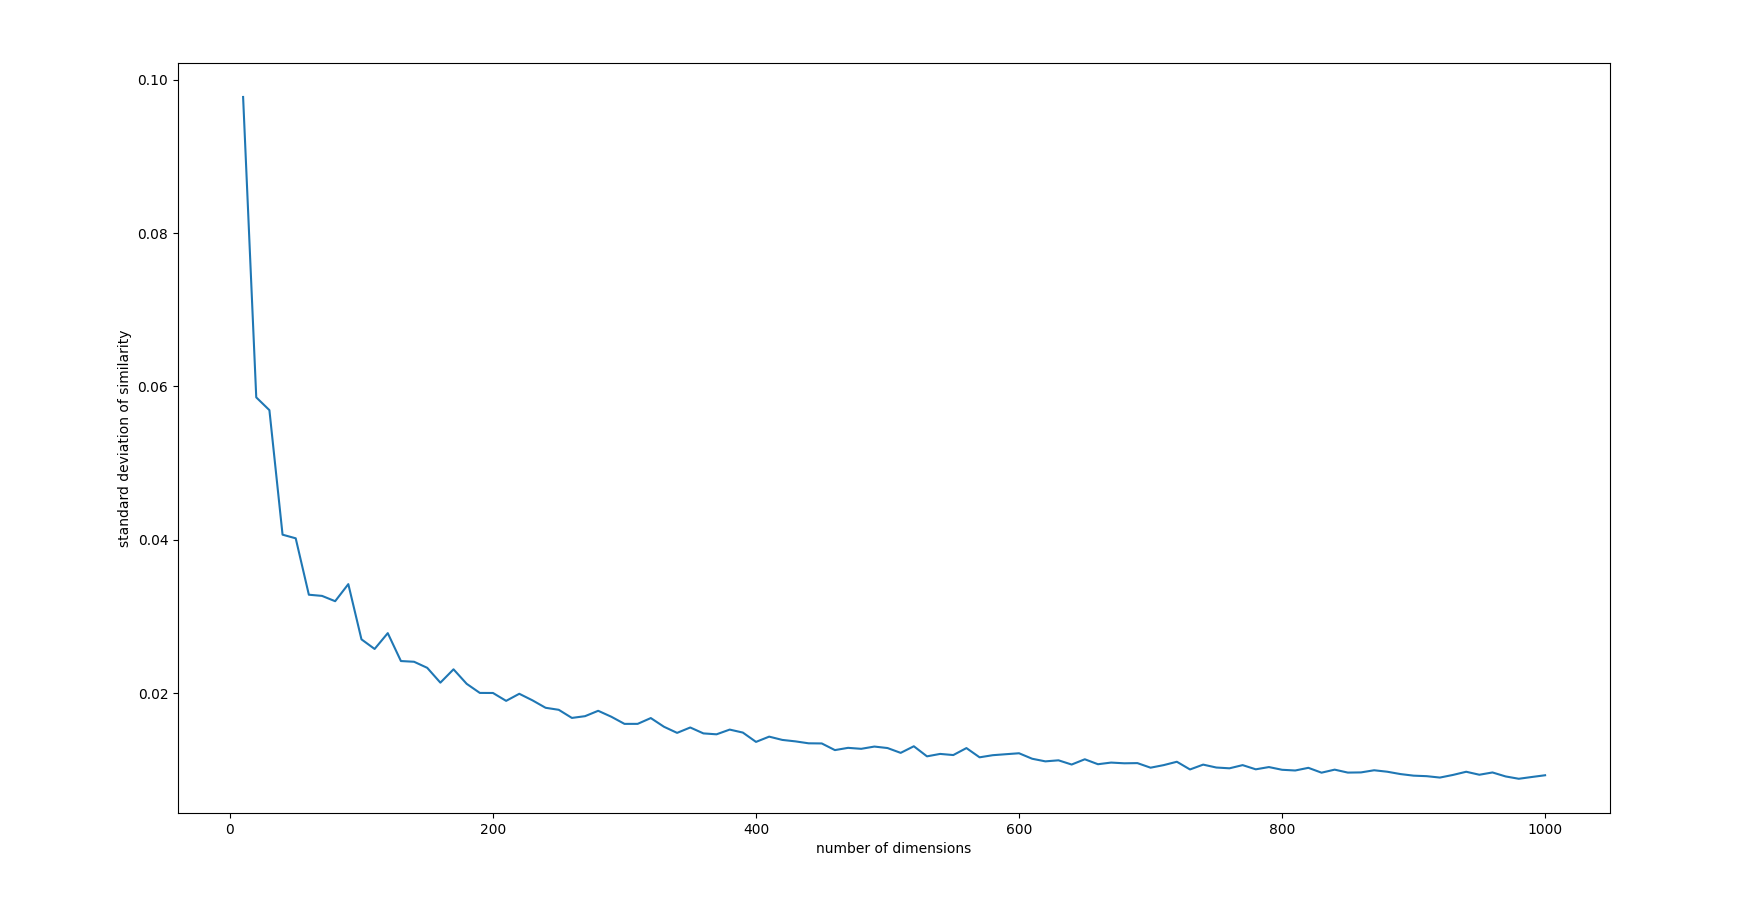
\includegraphics{../images/curseOfDimensionality.png}
\caption{curse of dimensionality, number of dimensions on the x axis, standard deviation of similarity on the y axis}
\end{figure}

\hypertarget{walkthrough-with-the-religion-dataset}{%
\chapter{Walkthrough with the religion dataset}\label{walkthrough-with-the-religion-dataset}}

\hypertarget{loading-and-understanding-the-dataset}{%
\section{Loading and understanding the dataset}\label{loading-and-understanding-the-dataset}}

We start with loading the libraries needed for the analysis.

\footnotesize

\begin{Shaded}
\begin{Highlighting}[]
\FunctionTok{library}\NormalTok{(ggplot2)}
\FunctionTok{library}\NormalTok{(ggthemes)}
\FunctionTok{library}\NormalTok{(rethinking)}
\FunctionTok{library}\NormalTok{(tidyverse)}
\FunctionTok{library}\NormalTok{(ggpubr)}
\FunctionTok{library}\NormalTok{(kableExtra)}
\FunctionTok{library}\NormalTok{(dplyr)}
\FunctionTok{library}\NormalTok{(ggExtra)}
\FunctionTok{library}\NormalTok{(cowplot)}
\end{Highlighting}
\end{Shaded}

\normalsize

We will use the choice of protected words and stereotypical predicates used in \protect\hyperlink{ref-Manzini2019blackToCriminal}{Manzini, Lim, Tsvetkov, \& Black} (\protect\hyperlink{ref-Manzini2019blackToCriminal}{2019}). This is a decent point of departure, as not only we want to compare our method to that of \protect\hyperlink{ref-Manzini2019blackToCriminal}{Manzini, Lim, Tsvetkov, \& Black} (\protect\hyperlink{ref-Manzini2019blackToCriminal}{2019}), but also because this data format is fairly general (as contrasted, say, with a set up for binary stereotypes). Note also that the method we develop here can fairly easily be run for different stereotypization patterns. Let's start with explaining the method and its deployment using a dataset obtained for the religion-related protected words.

Let's load, clean a bit and inspect the head of the religion dataset we prepared. In order to obtain this dataset, we calculated the cosine distance between each protected word and each word from both the bias-related attribute groups, which were used in the original study, and to neutral and human control attributes which we added as control groups. For instance, for religion, the bias-related predicates (coming from the original study in \protect\hyperlink{ref-Manzini2019blackToCriminal}{Manzini, Lim, Tsvetkov, \& Black} (\protect\hyperlink{ref-Manzini2019blackToCriminal}{2019})) include muslim bias attributes, jew bias attributes, christian bias attributes (see a list in the Appendix).

We decided to add control groups in the form of two classes --- neutral words and human-related words. Without a proper control group it is quite hard to compare the resulting cosine distances and decide on their significance in bias detection. We prepared approximately 230 neutral words to double-check the prima-facie neutral hypothesis that their cosine similarity to the protected words will oscillate around 0 (that is, the distances will be around 1). This provides us with a more reliable point of reference. Moreover, we added human attributes that are associated with people in general to investigate whether the smaller cosine distance between protected words and stereotypes can result simply from the fact that the stereotype predicates are associated with humans. For two control groups, we have randomly drawn 230 words that do not express any property usually attributed to humans, and human related attributes.

\pagebreak 
\vspace{1mm}
\footnotesize

\begin{table}

\caption{\label{tab:religionTableHead}Head of the religion dataset.}
\centering
\resizebox{\linewidth}{!}{
\begin{tabular}[t]{lllrrl}
\toprule
protectedWord & wordToCompare & wordClass & cosineDistance & cosineSimilarity & connection\\
\midrule
judaism & violent & muslim & 0.7141939 & 0.2858061 & different\\
judaism & terrorist & muslim & 0.7461333 & 0.2538667 & different\\
judaism & dirty & muslim & 1.2002599 & -0.2002599 & different\\
judaism & uneducated & muslim & 0.7885469 & 0.2114531 & different\\
judaism & greedy & jewish & 1.0026172 & -0.0026172 & associated\\
judaism & cheap & jewish & 1.2323229 & -0.2323229 & associated\\
\bottomrule
\end{tabular}}
\end{table}
\normalsize

The \texttt{protectedWord} column contains words from a protected class that (in a perfect world according to the assumptions of the orignal study) should not be associated with harmful stereotypes. \texttt{wordToCompare} contains attributes, including stereotypes and control group words. For each row we compute the cosine distances between a given protected word and a given attribute word. \texttt{wordClass} tells us which class an attribute is supposed to be stereotypically associated with, that is, whether the word from \texttt{wordToCompare} is associated stereotypically with jews, christians or muslims, or whether it belongs to a control group. \texttt{cosineDistance} is simply a calculation of the cosine distance between protected word and atrribute. \texttt{cosineSimilarity} contains the result of substracting cosine distance from 1. \texttt{connection} contains information about the relation type between a protected word and an attribute. If the attribute is e.g.~a harmful jewish stereotype and the protected word is also from the judaism group, the connection has value \texttt{associated}. If the attribute is still stereotypically jewish, but the protected word comes from another religion, the connection is labelled as \texttt{different}. If the attribute belongs to a neutral group then the connection is labelled as \texttt{none} and if an attribute belongs to the \texttt{human} class, then the connection is labelled as \texttt{human}.

\hypertarget{first-look-at-the-empirical-distributions}{%
\section{First look at the empirical distributions}\label{first-look-at-the-empirical-distributions}}

First let's take a look at the empirical distribution of distances by the connection type, initially ignoring the human control class for now.

\vspace{1mm}
\footnotesize

\begin{center}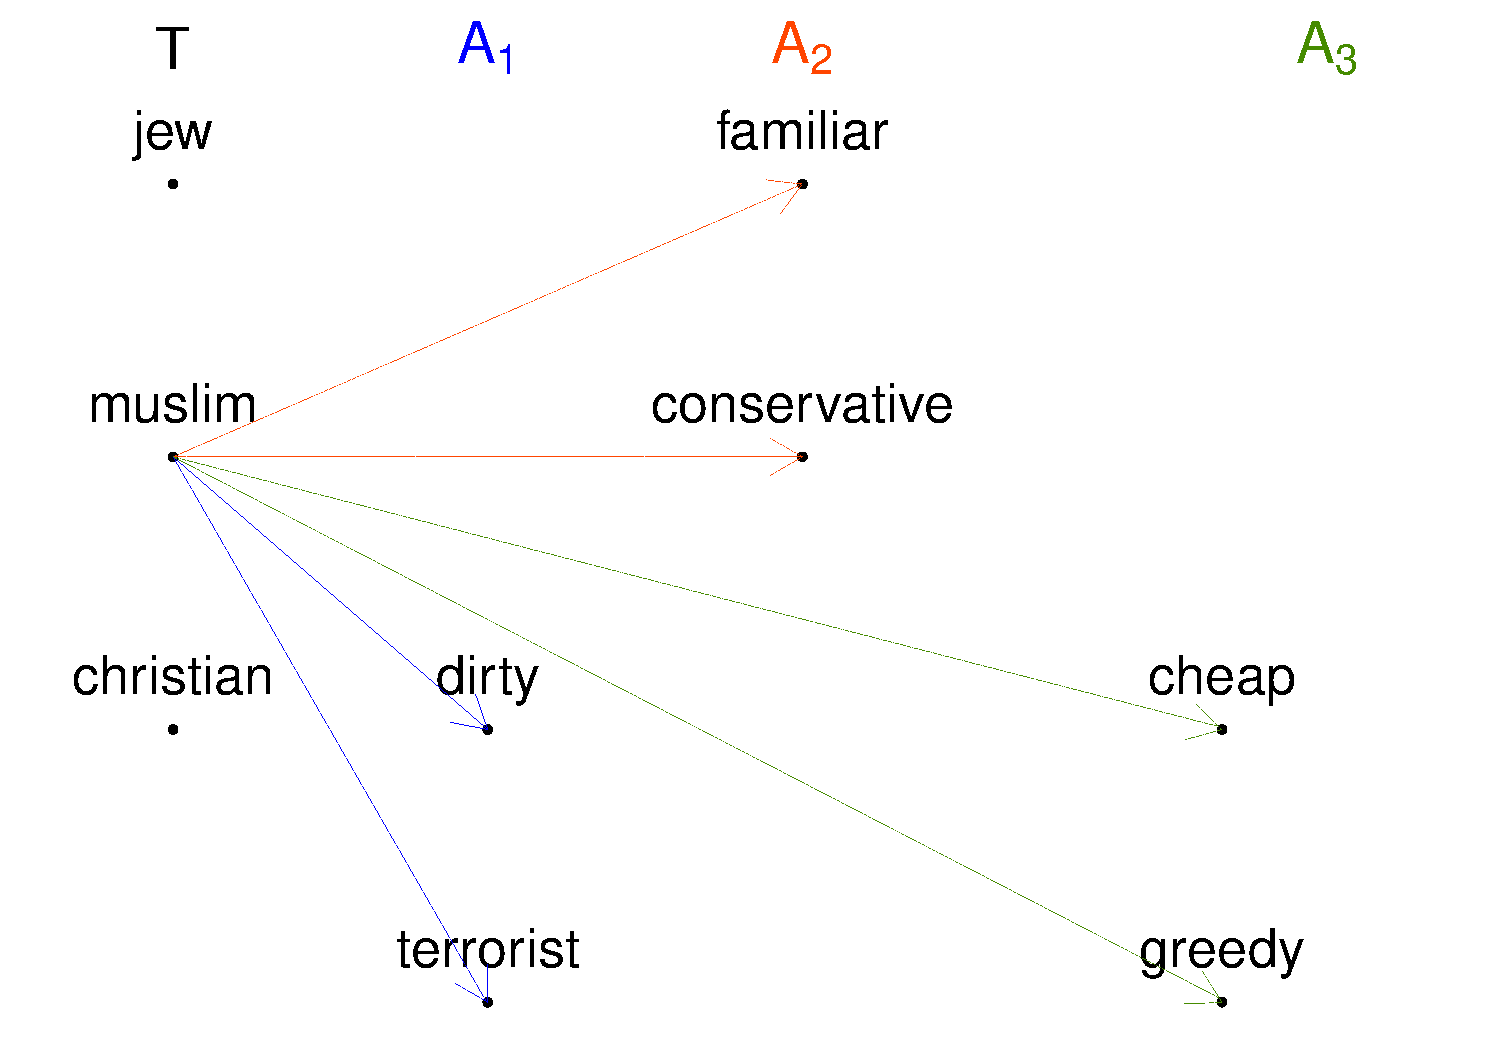
\includegraphics[width=1\linewidth]{_main_files/figure-latex/unnamed-chunk-3-1} \end{center}
\normalsize

The first impression is that while there is a shift for associated words towards smaller cosine distances as compared to the neutral words, slightly surprisingly a slightly weaker shift in the same direction is visible for attributes associated with different stereotypes. Moreover, the empirical distributions overlap to a large extent and the means grouped by connection type do not seem too far from each other. In fact, as there is a lot of variety in the cosine distances (as we will soon see), we need to gauge the uncertainty involved, and to look more carefully at individual protected words to get a better idea of how the cosine distance distribution changes for different attribute groups and different protected classes. Now, let's add the human attributes to the picture:

\vspace{1mm}
\footnotesize

\begin{center}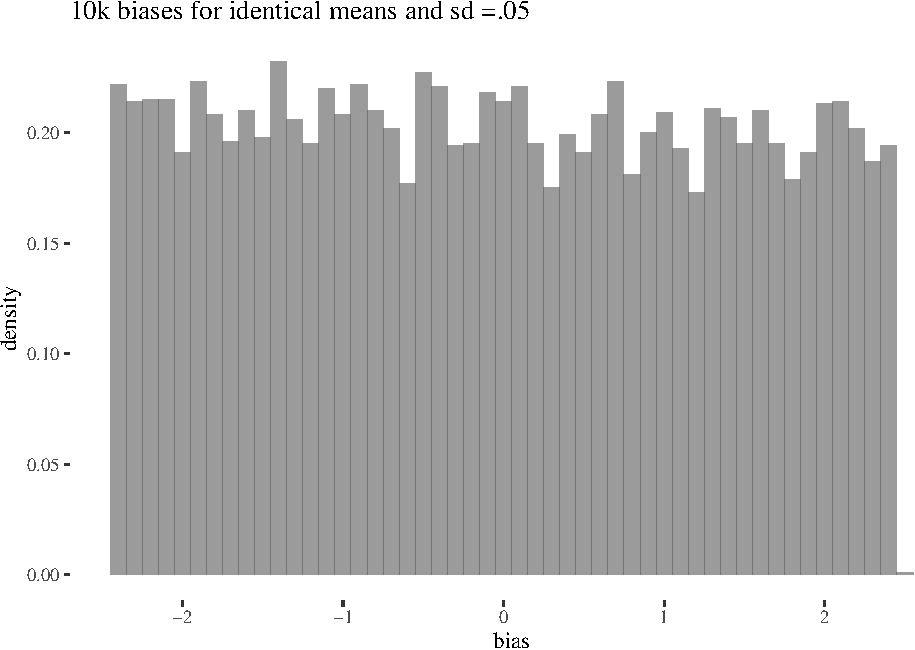
\includegraphics[width=1\linewidth]{_main_files/figure-latex/unnamed-chunk-4-1} \end{center}
\normalsize

\noindent Notice that the distribution for \texttt{human} (even though we did our best not to include in it any stereotype-related atributes) is left-skewed, with much overlap with \texttt{associated} and \texttt{different}, which illustrates the need to take being associated with humans as an important predictor.

Our focus lies in \texttt{connection} as a predictor. Morever, later on we'll be interested in looking at the protected words separately, and at protected words split by connection. For technical reasons it is useful to represent these factors as integer vectors.

\vspace{1mm}
\footnotesize

\begin{Shaded}
\begin{Highlighting}[]
\NormalTok{religion}\SpecialCharTok{$}\NormalTok{con }\OtherTok{\textless{}{-}} \FunctionTok{as.integer}\NormalTok{(religion}\SpecialCharTok{$}\NormalTok{connection)}
\end{Highlighting}
\end{Shaded}

\begin{verbatim}
## Warning: NAs introduced by coercion
\end{verbatim}

\begin{Shaded}
\begin{Highlighting}[]
\NormalTok{religion}\SpecialCharTok{$}\NormalTok{pw }\OtherTok{\textless{}{-}} \FunctionTok{as.integer}\NormalTok{(religion}\SpecialCharTok{$}\NormalTok{protectedWord)}
\end{Highlighting}
\end{Shaded}

\begin{verbatim}
## Warning: NAs introduced by coercion
\end{verbatim}

\begin{Shaded}
\begin{Highlighting}[]
\NormalTok{religion}\SpecialCharTok{$}\NormalTok{pwFactor }\OtherTok{\textless{}{-}} \FunctionTok{factor}\NormalTok{(}\FunctionTok{paste0}\NormalTok{(religion}\SpecialCharTok{$}\NormalTok{protectedWord, religion}\SpecialCharTok{$}\NormalTok{connection))}
\NormalTok{religion}\SpecialCharTok{$}\NormalTok{pwIndex }\OtherTok{\textless{}{-}} \FunctionTok{as.integer}\NormalTok{(religion}\SpecialCharTok{$}\NormalTok{pwFactor)}
\end{Highlighting}
\end{Shaded}

\normalsize

A short script, \texttt{cleanDataset} to make this faster, so equivalently:

\vspace{1mm}
\footnotesize

\begin{Shaded}
\begin{Highlighting}[]
\FunctionTok{source}\NormalTok{(}\StringTok{"../functions/cleanDataset.R"}\NormalTok{)}
\NormalTok{religion }\OtherTok{\textless{}{-}} \FunctionTok{read.csv}\NormalTok{(}\StringTok{"../datasets/religionReddit.csv"}\NormalTok{)[}\SpecialCharTok{{-}}\DecValTok{1}\NormalTok{]}
\NormalTok{religion }\OtherTok{\textless{}{-}} \FunctionTok{cleanDataset}\NormalTok{(religion,}\FunctionTok{c}\NormalTok{(}\StringTok{"christian"}\NormalTok{,}\StringTok{"human"}\NormalTok{,}\StringTok{"jewish"}\NormalTok{,}\StringTok{"muslim"}\NormalTok{,}\StringTok{"neutral"}\NormalTok{))}
\end{Highlighting}
\end{Shaded}

\begin{verbatim}
## Warning in cleanDataset(religion, c("christian", "human", "jewish", "muslim", :
## NAs introduced by coercion

## Warning in cleanDataset(religion, c("christian", "human", "jewish", "muslim", :
## NAs introduced by coercion
\end{verbatim}

\normalsize

\hypertarget{looking-at-the-islam-related-words}{%
\section{Looking at the islam-related words}\label{looking-at-the-islam-related-words}}

For now, let's focus on five protected words related to islam (``imam,'' ``islam,'' ``mosque,'' ``muslim,'' and ``quran''). The word list associates with islam four stereotypical attributes (``violent,'' ``terrorist,'' ``uneducated'' and ``dirty''). First, we select and plot the empirical distributions for these protected words.

\vspace{1mm}
\footnotesize

\begin{center}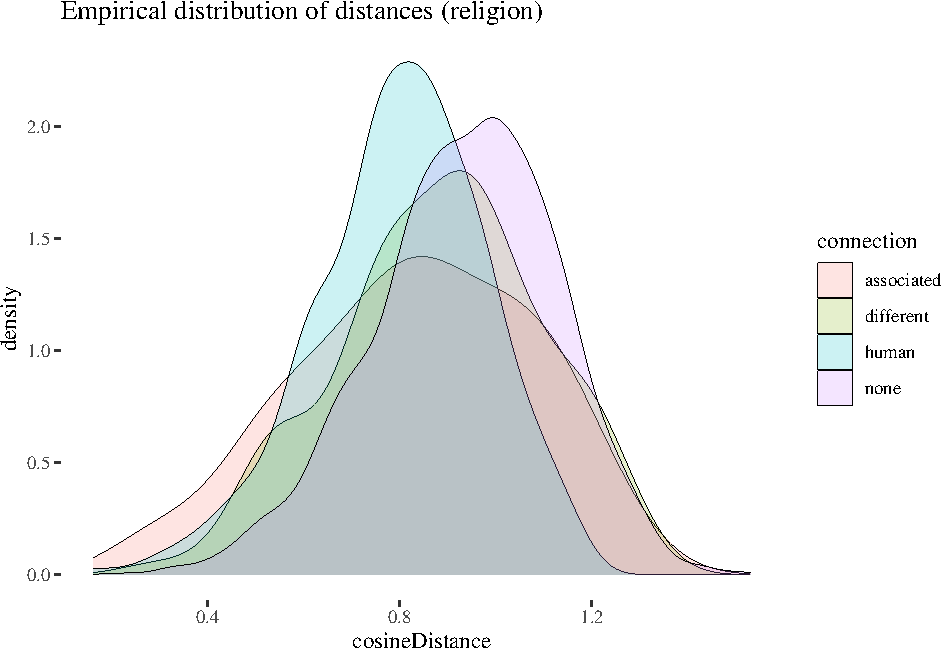
\includegraphics[width=1\linewidth]{_main_files/figure-latex/unnamed-chunk-7-1} \end{center}
\normalsize

\noindent Once we focus on words related to islam, the associated bias seems to be stronger than in the whole dataset. This is a step towards illustrating that the distribution of bias is uneven.

Now, say we want to look at a single protected word. Since the dataset also contains comparison multiple control neutral and human attributes, we randomly select only 5 from \texttt{none} and 5 from \texttt{human} control groups of those for the visualisation purposes.

\vspace{1mm}
\footnotesize

\begin{center}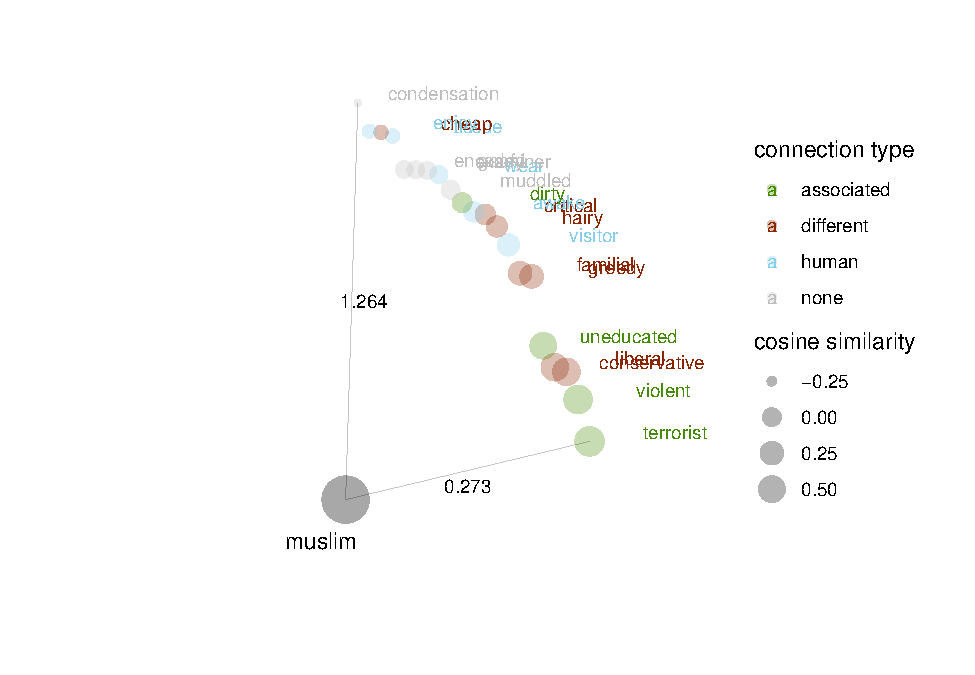
\includegraphics[width=1\linewidth]{_main_files/figure-latex/tableMuslimActive-1} \end{center}
\normalsize

Note that the distance between the grey point and the other points is proportional to cosine distance, the non-grey point size is proportional to cosine similarity to the protected word, and color groups by the connection type. So for \texttt{muslim} it seems that the stereotypes coming from the word list are fairly well visible. To give you some taste of how uneven the dataset is, compare this to what happens with \texttt{priest}.

\vspace{1mm}
\footnotesize

\begin{center}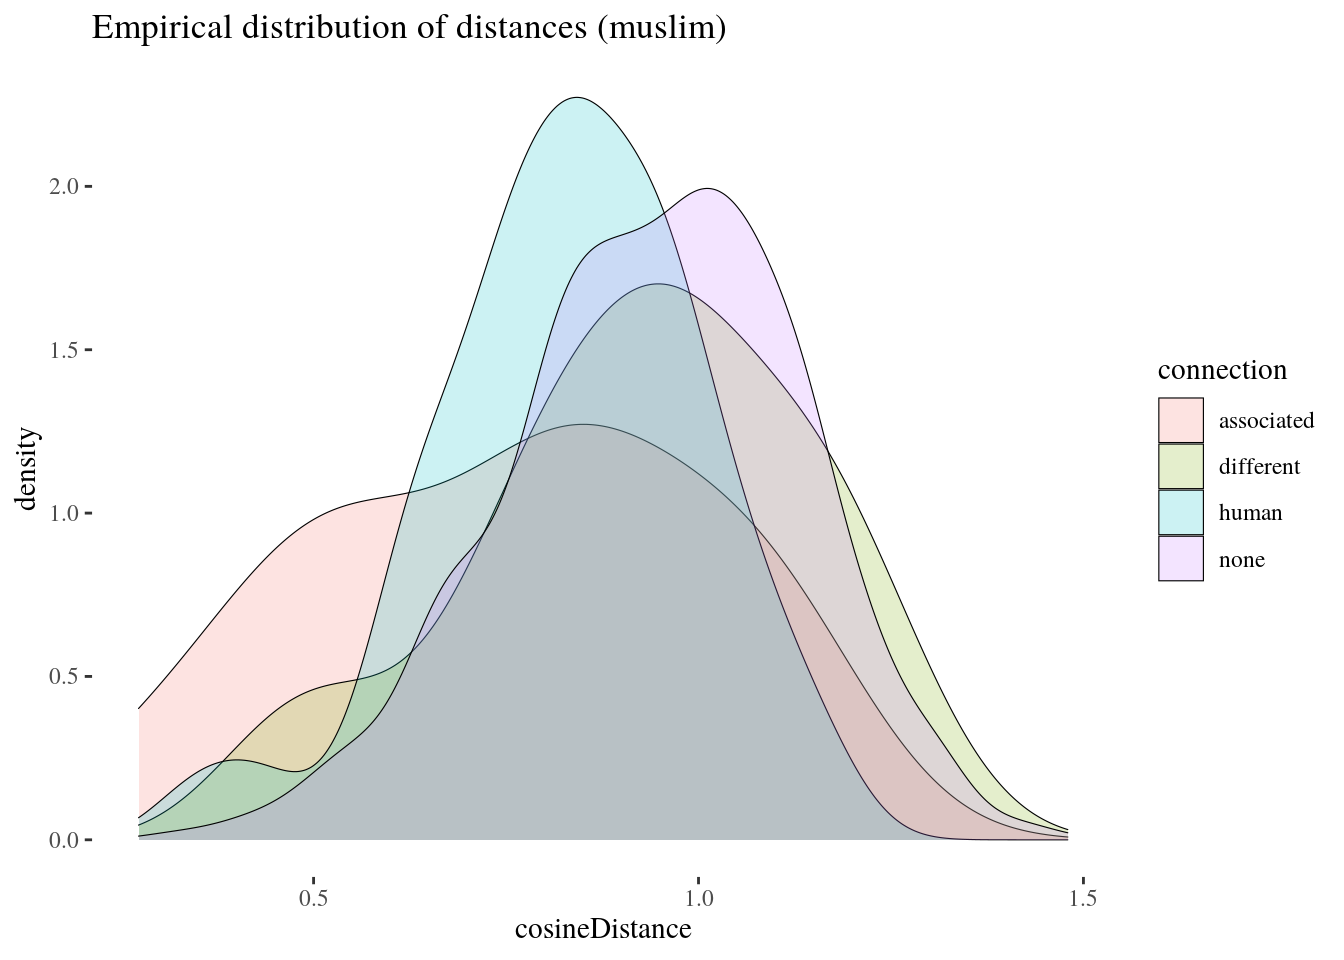
\includegraphics[width=1\linewidth]{_main_files/figure-latex/unnamed-chunk-8-1} \end{center}
\normalsize

\noindent Here you can see that some human attributes are closer than stereotype attributes, and that there is no clear reason to claim that \texttt{associated} attributes are closer than \texttt{different} or \texttt{human} attributes. This, again, illustrates the need of case-by-case analysis with control groups.

The general idea now is that the word lists provided in different pieces of research are just samples of attributes associates with various stereotypes and should be treated as such: the uncertainty involved and the sample sizes should have clear impact on our estimates.

\hypertarget{bayesian-model-structure-and-assumptions}{%
\section{Bayesian model structure and assumptions}\label{bayesian-model-structure-and-assumptions}}

We will now think of cosine distance as the output variable, and
will build a few Bayesian models to compare. First, we just build a baseline model which estimates cosine distance to the attributes separately for each protected word. The underlying idea is that different protected words might in general have different relations to all the attributes and these relations should be our point of departure.\footnote{The construction of the Bayesian models and code for visualisations is due to Rafal Urbaniak.}

Here is the intuition behind the mathematical Bayesian model involved. Our outcome variable is \texttt{cosine\ difference}, which we take to me normally distributed around the predicted mean for a given protected word (that is, we assume the residuals are normally distributed). The simplest model specification is:

\begin{align}
cosineDistance_i  & \sim dnorm(\mu_i, \sigma) \\
\mu_i & = m_{pw} \\
m_{pw} & ~ dnorm(1,.5) \\
\sigma &\sim  dcauchy(0,1)
\end{align}

That is, we assume the estimated means might be different for diferent protected words and our prior for the mean and the overal standard deviation are normal with mean 1 and sd=.5 and half-cauchy with parameters \texttt{0,1}. Further on we'll also estimate additional impact the connection type may have. For this impact we take a slightly skeptical prior centered around 0 distributed normally with sd = 1. These are fairly weak and slightly skeptical regularizing priors, which can be illustrated as follows:

\vspace{2mm}

\begin{center}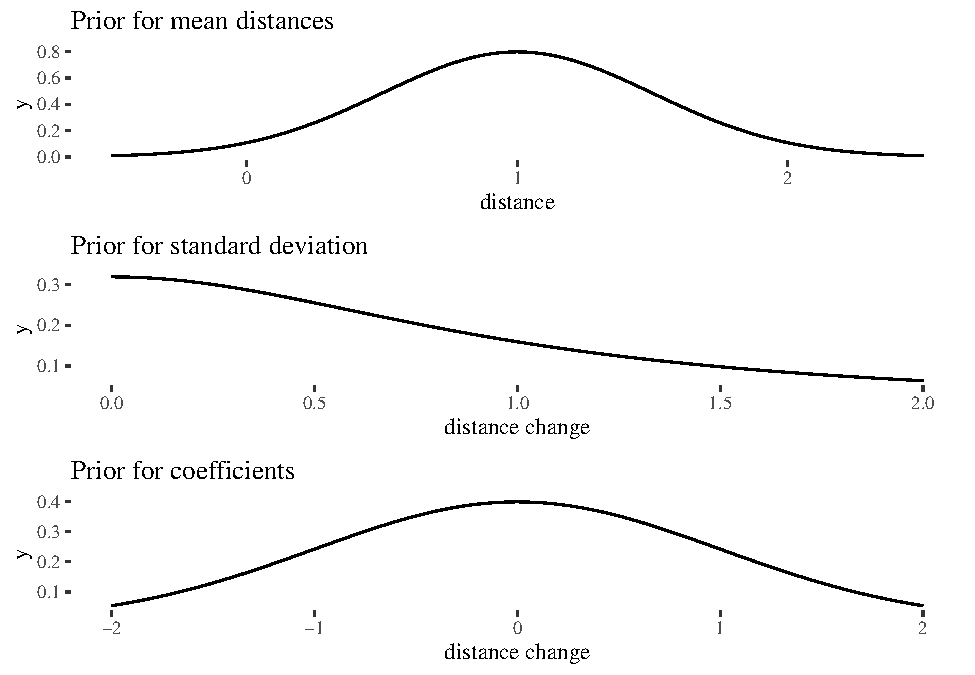
\includegraphics[width=1\linewidth]{_main_files/figure-latex/priorsVis-1} \end{center}

\hypertarget{choosing-predictors}{%
\section{Choosing predictors}\label{choosing-predictors}}

Now we can define and compile the baseline model. Its parameters will have a posterior distribution obtained using either Hamiltionian Monte Carlo methods (STAN) available through the \texttt{rethinking} package.

\vspace{1mm}
\footnotesize

\begin{Shaded}
\begin{Highlighting}[]
\FunctionTok{library}\NormalTok{(rethinking)}
\FunctionTok{options}\NormalTok{(}\AttributeTok{buildtools.check =} \ControlFlowTok{function}\NormalTok{(action) }\ConstantTok{TRUE}\NormalTok{ )}
\NormalTok{religionBaseline }\OtherTok{\textless{}{-}} \FunctionTok{ulam}\NormalTok{(}
  \FunctionTok{alist}\NormalTok{(}
\NormalTok{    cosineDistance }\SpecialCharTok{\textasciitilde{}} \FunctionTok{dnorm}\NormalTok{(mu,sigma),}
\NormalTok{    mu }\OtherTok{\textless{}{-}}\NormalTok{ m[pw],}
\NormalTok{    m[pw] }\SpecialCharTok{\textasciitilde{}} \FunctionTok{dnorm}\NormalTok{(}\DecValTok{1}\NormalTok{,.}\DecValTok{5}\NormalTok{),}
\NormalTok{    sigma }\SpecialCharTok{\textasciitilde{}} \FunctionTok{dcauchy}\NormalTok{(}\DecValTok{0}\NormalTok{,}\DecValTok{1}\NormalTok{)}
\NormalTok{  ),}
  \AttributeTok{data =}\NormalTok{ religion,}
  \AttributeTok{chains=}\DecValTok{2}\NormalTok{ , }\AttributeTok{iter=}\DecValTok{4000}\NormalTok{ , }\AttributeTok{warmup=}\DecValTok{1000}\NormalTok{,}
  \AttributeTok{start=} \FunctionTok{list}\NormalTok{(}\AttributeTok{mu =} \DecValTok{1}\NormalTok{, }\AttributeTok{co =} \DecValTok{0}\NormalTok{, }\AttributeTok{sigma=}\NormalTok{ .}\DecValTok{3}\NormalTok{),}
  \AttributeTok{log\_lik =} \ConstantTok{TRUE}\NormalTok{, }\AttributeTok{cores=}\DecValTok{4}
\NormalTok{)}
\CommentTok{\#saving}
\CommentTok{\#saveRDS(religionBaseline, }
\CommentTok{\#file = "cosineAnalysis/models/religionBaseline.rds")}
\end{Highlighting}
\end{Shaded}

\normalsize

The only reason we need it is the evaluation of connection as a predictor. Does including it in o the model improve the situation? To investigate this, let's now build a model according to the following specification:

\begin{align}
cosineDistance_i  & \sim dnorm(\mu_i, \sigma) \\
\mu_i & = m_{pw} + co_{con}\\
m_{pw} & ~ dnorm(1,.5) \\
co_{con} & ~ dnorm(0,1) \\
\sigma &\sim  dcauchy(0,1)
\end{align}

\noindent The idea now is that each connection type comes with its own coefficient \(co\) that has impact on mean distances for protected words taken separately.

\vspace{1mm}
\footnotesize

\begin{Shaded}
\begin{Highlighting}[]
\FunctionTok{library}\NormalTok{(rethinking)}
\FunctionTok{options}\NormalTok{(}\AttributeTok{buildtools.check =} \ControlFlowTok{function}\NormalTok{(action) }\ConstantTok{TRUE}\NormalTok{ )}
\NormalTok{religionCoefs }\OtherTok{\textless{}{-}} \FunctionTok{ulam}\NormalTok{(}
  \FunctionTok{alist}\NormalTok{(}
\NormalTok{    cosineDistance }\SpecialCharTok{\textasciitilde{}} \FunctionTok{dnorm}\NormalTok{(mu,sigma),}
\NormalTok{    mu }\OtherTok{\textless{}{-}}\NormalTok{ m[pw] }\SpecialCharTok{+}\NormalTok{ co[con],}
\NormalTok{    m[pw] }\SpecialCharTok{\textasciitilde{}} \FunctionTok{dnorm}\NormalTok{(}\DecValTok{1}\NormalTok{,.}\DecValTok{5}\NormalTok{),}
\NormalTok{    co[con] }\SpecialCharTok{\textasciitilde{}}\FunctionTok{dnorm}\NormalTok{(}\DecValTok{0}\NormalTok{,.}\DecValTok{5}\NormalTok{),}
\NormalTok{    sigma }\SpecialCharTok{\textasciitilde{}} \FunctionTok{dcauchy}\NormalTok{(}\DecValTok{0}\NormalTok{,}\DecValTok{1}\NormalTok{)}
\NormalTok{  ),}
  \AttributeTok{data =}\NormalTok{ religion,}
  \AttributeTok{chains=}\DecValTok{2}\NormalTok{ , }\AttributeTok{iter=}\DecValTok{8000}\NormalTok{ , }\AttributeTok{warmup=}\DecValTok{1000}\NormalTok{, }
  \AttributeTok{log\_lik =} \ConstantTok{TRUE}
\NormalTok{)}
\end{Highlighting}
\end{Shaded}

\normalsize

\noindent First, let's see if this model is really better in terms of the Widely Acceptable Information Criterion (WAIC):

\vspace{1mm}
\footnotesize

\begin{verbatim}
##                   WAIC SE dWAIC dSE pWAIC weight
## religionCoefs    -2328 93     0  NA    20      1
## religionBaseline -2283 95    45  17    16      0
\end{verbatim}

\normalsize

Clearly, it should be given weight 1 as compared to the baseline model. So far, we've learned that the connection type actually has predictive value. Let's take a look at the coefficient estimates:

\vspace{1mm}
\footnotesize

\begin{verbatim}
##              mean        sd       5.5%      94.5%    n_eff    Rhat4
## co[1] -0.14956420 0.1151675 -0.3261650 0.03741930 294.2033 1.001449
## co[2] -0.09880543 0.1145024 -0.2736985 0.08813271 291.5044 1.001564
## co[3] -0.07282752 0.1133894 -0.2447778 0.11158986 287.7820 1.001627
## co[4] -0.03103179 0.1131420 -0.2034442 0.15268770 286.8283 1.001606
\end{verbatim}

\normalsize

\hypertarget{dataset-level-coefficients}{%
\section{\texorpdfstring{Dataset-level coefficients \label{sec:datasetsLevelCoeffs}}{Dataset-level coefficients }}\label{dataset-level-coefficients}}

\noindent Let's plot them together with their highest posterior density invervals, for the three topic groups.

\begin{center}
\begin{figure}[!htb]\centering
   \begin{minipage}{0.55\textwidth}
  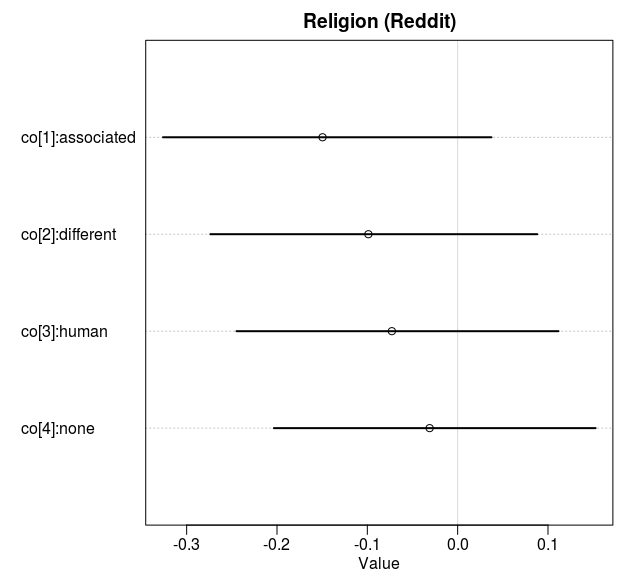
\includegraphics[width=7cm]{../images/religionCoeffs.jpeg}
   \end{minipage}
   \begin {minipage}{0.43\textwidth}
    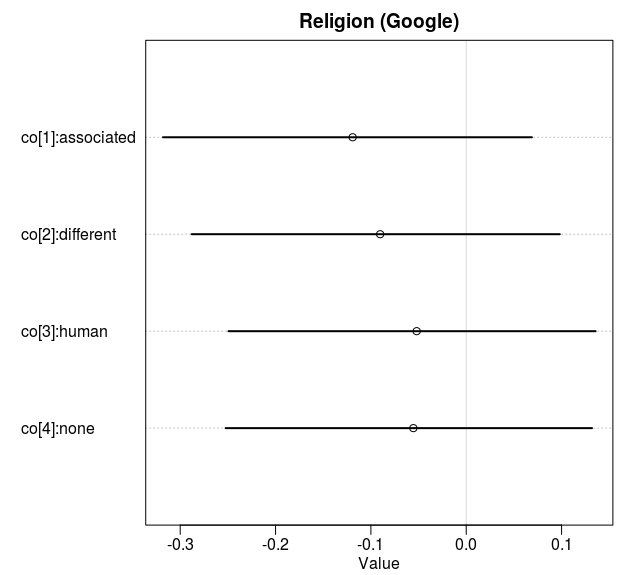
\includegraphics[width=7cm]{../images/religionGoogleCoeffs.jpeg}
   \end{minipage}
   
   
  \begin{minipage}{0.55\textwidth}
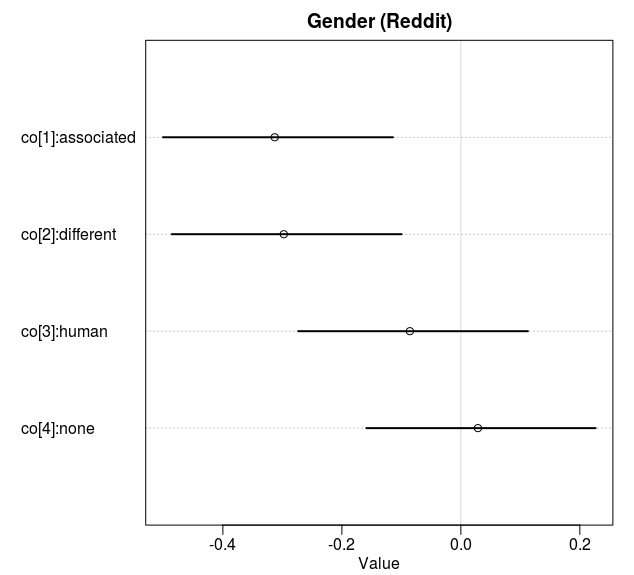
\includegraphics[width=7cm]{../images/genderCoeffs.jpeg}
\end{minipage}
   \begin {minipage}{0.43\textwidth}
    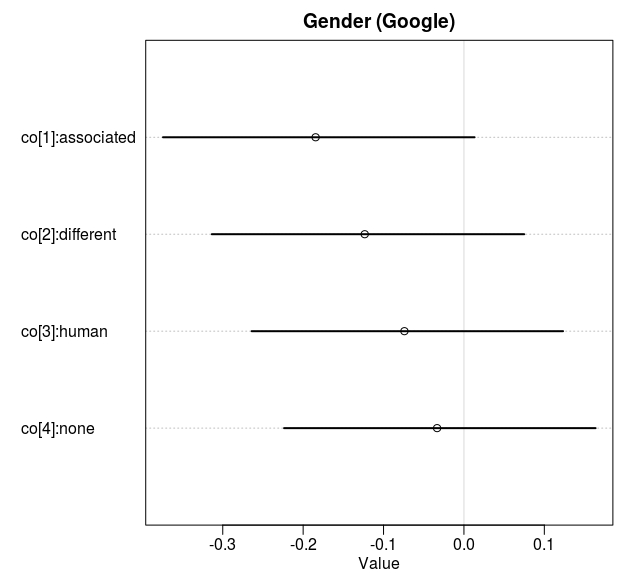
\includegraphics[width=7cm]{../images/genderGoogleCoeffs.jpeg}
   \end{minipage}
   
   
   
   
  \begin{minipage}{0.55\textwidth}
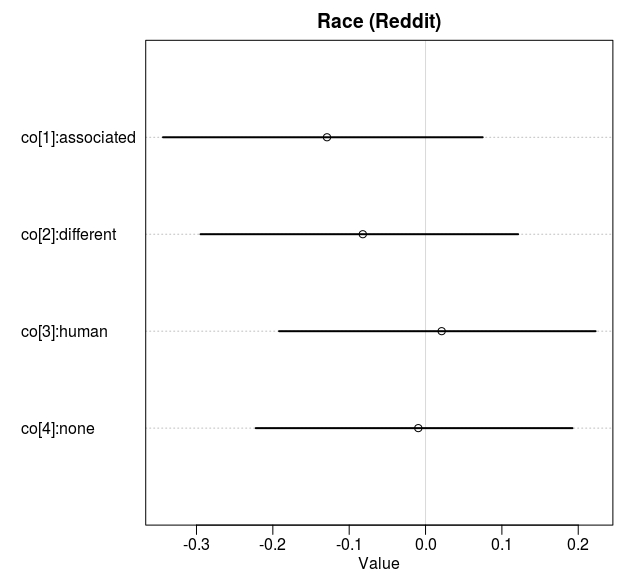
\includegraphics[width=7cm]{../images/raceCoeffs.jpeg}
\end{minipage}
   \begin {minipage}{0.43\textwidth}
    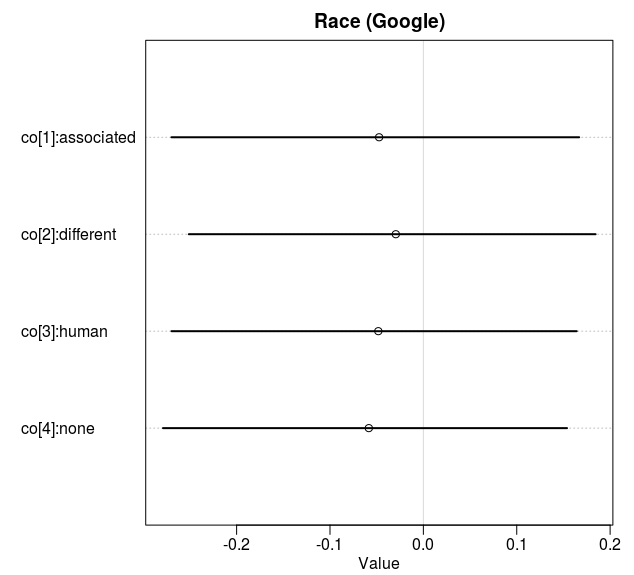
\includegraphics[width=7cm]{../images/raceGoogleCoeffs.jpeg}
   \end{minipage}
\end{figure}


\end{center}

\noindent What should strike us is that while the mean estimates of the coefficients indeed do differ a bit, usually the highest posterior density invervals all include zero, and so we do not have strong reasons to say that, say, as far as the whole religion dataset is involved, being associated indeed is connected with lower cosine distance. A second striking observation is that the estimated impact for associated stereotypes is quite often not too different from the estimated impact of attributes associated with different stereotypes, and both are sometimes not too far from the estimated impact for simply human attributes. In general, once the uncertainty involved is taken seriously by using control groups and statistical uncertainty estimation that does not dispose of pointwise data, the picture which focuses only on differences between means of means is too simplistic.

But this doesn't mean important differences for some protected words are not there. For one thing, if you start with a word list that is very uneven, the actually not so bad status of some of the protected words might mask a pretty bad situation in which some other protected words are. For comparison, let's see what a model focused on words related to islam tells us.

\vspace{1mm}
\footnotesize

\begin{Shaded}
\begin{Highlighting}[]
\CommentTok{\#this is how we build the model}
\NormalTok{religion }\OtherTok{\textless{}{-}} \FunctionTok{read.csv}\NormalTok{(}\StringTok{"cosineAnalysis/datasets/religionReddit.csv"}\NormalTok{)[}\SpecialCharTok{{-}}\DecValTok{1}\NormalTok{]}
\FunctionTok{colnames}\NormalTok{(religion) }\OtherTok{\textless{}{-}} \FunctionTok{c}\NormalTok{(}\StringTok{"protectedWord"}\NormalTok{,}\StringTok{"wordToCompare"}\NormalTok{,}\StringTok{"wordClass"}\NormalTok{,}
                        \StringTok{"cosineDistance"}\NormalTok{,}\StringTok{"cosineSimilarity"}\NormalTok{,}\StringTok{"connection"}\NormalTok{)}
\FunctionTok{levels}\NormalTok{(religion}\SpecialCharTok{$}\NormalTok{wordClass) }\OtherTok{\textless{}{-}} \FunctionTok{c}\NormalTok{(}\StringTok{"christian"}\NormalTok{,}\StringTok{"human"}\NormalTok{,}\StringTok{"jewish"}\NormalTok{,}\StringTok{"muslim"}\NormalTok{,}\StringTok{"neutral"}\NormalTok{)}
\NormalTok{muslimWords }\OtherTok{\textless{}{-}} \FunctionTok{c}\NormalTok{(}\StringTok{"imam"}\NormalTok{,}\StringTok{"islam"}\NormalTok{,}\StringTok{"mosque"}\NormalTok{,}\StringTok{"muslim"}\NormalTok{,}\StringTok{"quran"}\NormalTok{)}
\NormalTok{muslim }\OtherTok{\textless{}{-}}\NormalTok{ religion }\SpecialCharTok{\%\textgreater{}\%} \FunctionTok{filter}\NormalTok{(protectedWord }\SpecialCharTok{\%in\%}\NormalTok{ muslimWords)}
\NormalTok{muslim}\SpecialCharTok{$}\NormalTok{protectedWord }\OtherTok{\textless{}{-}} \FunctionTok{droplevels}\NormalTok{(muslim}\SpecialCharTok{$}\NormalTok{protectedWord)}
\NormalTok{muslim}\SpecialCharTok{$}\NormalTok{pw }\OtherTok{\textless{}{-}} \FunctionTok{as.integer}\NormalTok{(muslim}\SpecialCharTok{$}\NormalTok{protectedWord)}
\NormalTok{muslim}\SpecialCharTok{$}\NormalTok{con }\OtherTok{\textless{}{-}} \FunctionTok{as.integer}\NormalTok{(muslim}\SpecialCharTok{$}\NormalTok{connection)}
\NormalTok{muslim}\SpecialCharTok{$}\NormalTok{pwFactor }\OtherTok{\textless{}{-}} \FunctionTok{factor}\NormalTok{(}\FunctionTok{paste0}\NormalTok{(muslim}\SpecialCharTok{$}\NormalTok{protectedWord, muslim}\SpecialCharTok{$}\NormalTok{connection))}
\NormalTok{muslim}\SpecialCharTok{$}\NormalTok{pwIndex }\OtherTok{\textless{}{-}} \FunctionTok{as.integer}\NormalTok{(muslim}\SpecialCharTok{$}\NormalTok{pwFactor)}

\NormalTok{islamCoefs }\OtherTok{\textless{}{-}} \FunctionTok{ulam}\NormalTok{(}
  \FunctionTok{alist}\NormalTok{(}
\NormalTok{    cosineDistance }\SpecialCharTok{\textasciitilde{}} \FunctionTok{dnorm}\NormalTok{(mu,sigma),}
\NormalTok{    mu }\OtherTok{\textless{}{-}}\NormalTok{ m[pw] }\SpecialCharTok{+}\NormalTok{ co[con],}
\NormalTok{    m[pw] }\SpecialCharTok{\textasciitilde{}} \FunctionTok{dnorm}\NormalTok{(}\DecValTok{1}\NormalTok{,.}\DecValTok{5}\NormalTok{),}
\NormalTok{    co[con] }\SpecialCharTok{\textasciitilde{}}\FunctionTok{dnorm}\NormalTok{(}\DecValTok{0}\NormalTok{,.}\DecValTok{5}\NormalTok{),}
\NormalTok{    sigma }\SpecialCharTok{\textasciitilde{}} \FunctionTok{dcauchy}\NormalTok{(}\DecValTok{0}\NormalTok{,}\DecValTok{1}\NormalTok{)}
\NormalTok{  ),}
  \AttributeTok{data =}\NormalTok{ muslim,}
  \AttributeTok{chains=}\DecValTok{2}\NormalTok{ , }\AttributeTok{iter=}\DecValTok{10000}\NormalTok{ , }\AttributeTok{warmup=}\DecValTok{1000}\NormalTok{, }\AttributeTok{cores =} \DecValTok{4}\NormalTok{,}
  \AttributeTok{log\_lik =} \ConstantTok{TRUE}
\NormalTok{)}
\end{Highlighting}
\end{Shaded}

\normalsize

Let's take a look at the coefficients:

\vspace{1mm}
\footnotesize

\begin{verbatim}
##                mean        sd       5.5%      94.5%    n_eff    Rhat4
## co[1] -0.1979930035 0.1708785 -0.4682696 0.07634977 1789.894 1.003445
## co[2] -0.0334215769 0.1687587 -0.3021954 0.23720938 1738.720 1.003575
## co[3] -0.0192492753 0.1675754 -0.2840596 0.24860974 1732.907 1.003755
## co[4] -0.0003911363 0.1670610 -0.2661047 0.26815172 1723.758 1.003837
\end{verbatim}

\normalsize

\begin{center}
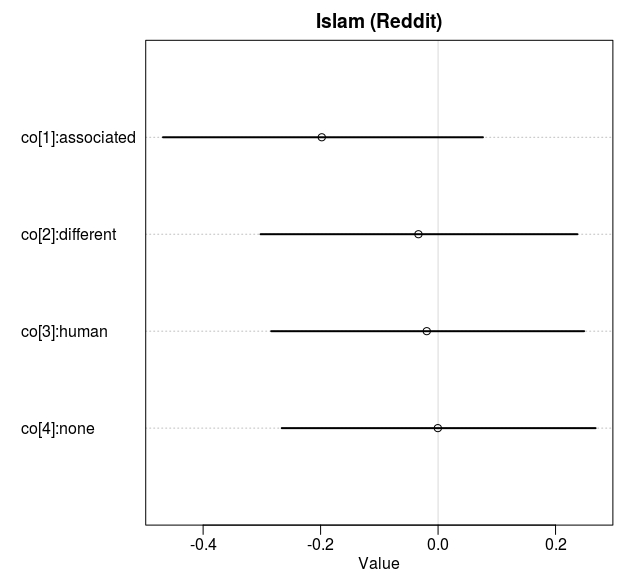
\includegraphics[width=8cm]{../images/islamCoeffs.jpeg}
\end{center}

\normalsize

While muslim words were unusual in the sense that the disparity between associated attributes and others is stronger, the evidence is still not conclusive. This is because the variation even within islam-related words is large enough (and sample sizes sufficiently small) for all the highest posterior density invervals to still include zeros.

So, it seems, taking a closer look does seem to make a difference. The question is, what happens if we do take a close look at the level of protected words?

\hypertarget{protected-word-level-analysis}{%
\chapter{Protected-word level analysis}\label{protected-word-level-analysis}}

\hypertarget{model-structure-and-assumptions}{%
\section{Model structure and assumptions}\label{model-structure-and-assumptions}}

Let's turn then to data analysis that takes a look at protected words separately. This time, for each combination of a protected word and a connection status we will have a separate mean cosine distance estimate, each coming with its own highest posterior density interval. This means we will use indices that are result from all such combinations (and then we will split them up in the model precis to build visualisation, feel free to look at the \texttt{visualiseStats.R} script for details).

\vspace{1mm}
\footnotesize

\begin{Shaded}
\begin{Highlighting}[]
\FunctionTok{options}\NormalTok{(}\AttributeTok{buildtools.check =} \ControlFlowTok{function}\NormalTok{(action) }\ConstantTok{TRUE}\NormalTok{ ) }\CommentTok{\#removes install pop{-}up request}
\NormalTok{religion}\SpecialCharTok{$}\NormalTok{pwFactor }\OtherTok{\textless{}{-}} \FunctionTok{factor}\NormalTok{(}\FunctionTok{paste0}\NormalTok{(religion}\SpecialCharTok{$}\NormalTok{protectedWord, }\StringTok{"{-}"}\NormalTok{, religion}\SpecialCharTok{$}\NormalTok{connection))}
\NormalTok{religion}\SpecialCharTok{$}\NormalTok{pwIndex }\OtherTok{\textless{}{-}} \FunctionTok{as.integer}\NormalTok{(religion}\SpecialCharTok{$}\NormalTok{pwFactor)}

\NormalTok{religionSeparate }\OtherTok{\textless{}{-}} \FunctionTok{ulam}\NormalTok{(}
  \FunctionTok{alist}\NormalTok{(}
\NormalTok{    cosineDistance }\SpecialCharTok{\textasciitilde{}} \FunctionTok{dnorm}\NormalTok{(mu,sigma),}
\NormalTok{    mu }\OtherTok{\textless{}{-}}\NormalTok{ c[pwIndex],}
\NormalTok{    c[pwIndex] }\SpecialCharTok{\textasciitilde{}} \FunctionTok{dnorm}\NormalTok{(}\DecValTok{1}\NormalTok{,.}\DecValTok{5}\NormalTok{),}
\NormalTok{    sigma }\SpecialCharTok{\textasciitilde{}} \FunctionTok{dcauchy}\NormalTok{(}\DecValTok{0}\NormalTok{,}\DecValTok{1}\NormalTok{)}
\NormalTok{  ),}
  \AttributeTok{data =}\NormalTok{ religion,}
  \AttributeTok{chains=}\DecValTok{2}\NormalTok{ , }\AttributeTok{iter=}\DecValTok{10000}\NormalTok{ , }\AttributeTok{warmup=}\DecValTok{1000}\NormalTok{,}
  \AttributeTok{start=}\FunctionTok{list}\NormalTok{(}\AttributeTok{no =} \DecValTok{1}\NormalTok{, }\AttributeTok{a =} \DecValTok{0}\NormalTok{, }\AttributeTok{d =} \DecValTok{0}\NormalTok{, }\AttributeTok{sigma=}\NormalTok{ .}\DecValTok{3}\NormalTok{), }\AttributeTok{log\_lik =}  \ConstantTok{TRUE}
\NormalTok{)}
\end{Highlighting}
\end{Shaded}

\normalsize

\noindent Let's see if the individualized model does better than the previous models in light of WAIC which does add penalty for the number of parameters.

\vspace{1mm}
\footnotesize

\begin{Shaded}
\begin{Highlighting}[]
\NormalTok{compareBaselineCoefsSeparate}\OtherTok{\textless{}{-}} \FunctionTok{readRDS}\NormalTok{(}\StringTok{"../datasets/compareBaselineCoefsSeparate.rds"}\NormalTok{)}
\NormalTok{compareBaselineCoefsSeparate}
\end{Highlighting}
\end{Shaded}

\begin{verbatim}
##                   WAIC SE dWAIC dSE pWAIC weight
## religionSeparate -2400 93     0  NA    60      1
## religionCoefs    -2328 93    72  29    20      0
## religionBaseline -2283 95   117  37    16      0
\end{verbatim}

\normalsize

\hypertarget{protected-classes-in-reddit-and-google-embeddings}{%
\section{Protected classes in Reddit and Google embeddings}\label{protected-classes-in-reddit-and-google-embeddings}}

It seems that we do want to prefer this model, despite its relative complication. Now, what does it tell us about the protected words? Let's visualise the predicted means together with 89\% highest posterior density intervals.

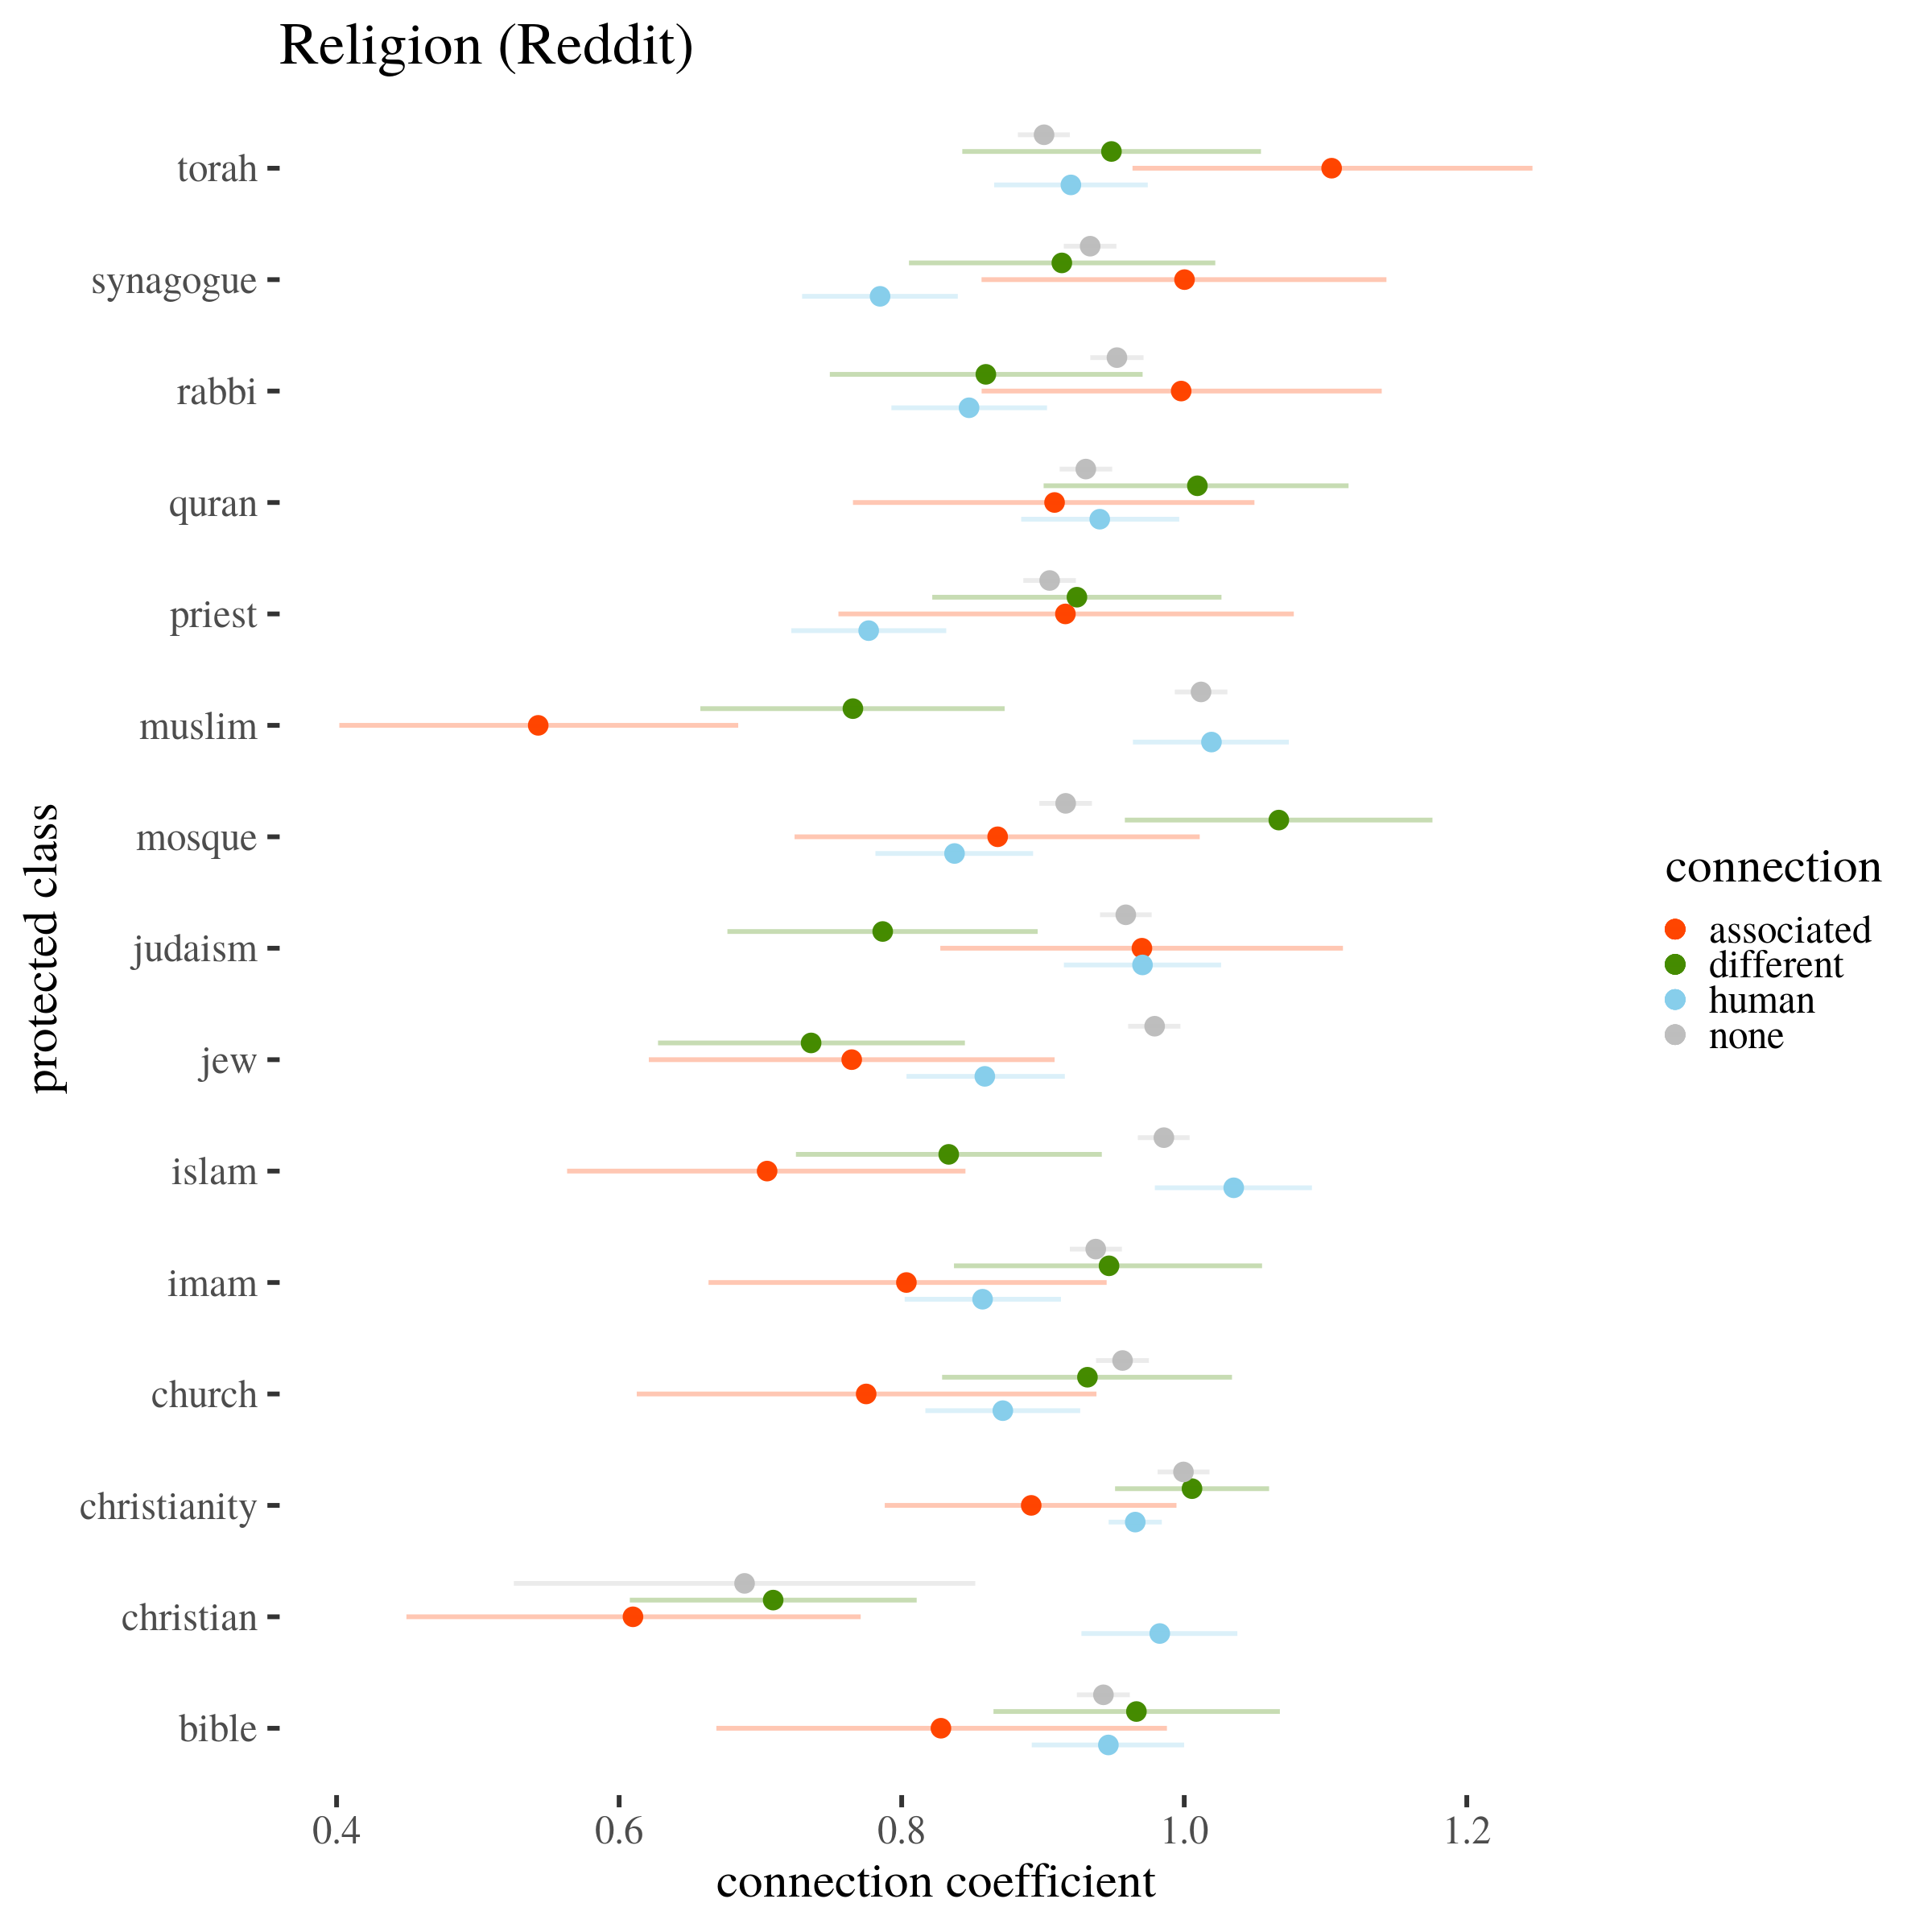
\includegraphics[width=14cm]{../images/visReligionReddit.png}

Before we move on, let's perform analogous analyses for the remaining types of supposed bias: gender and race (the model building is analogous).

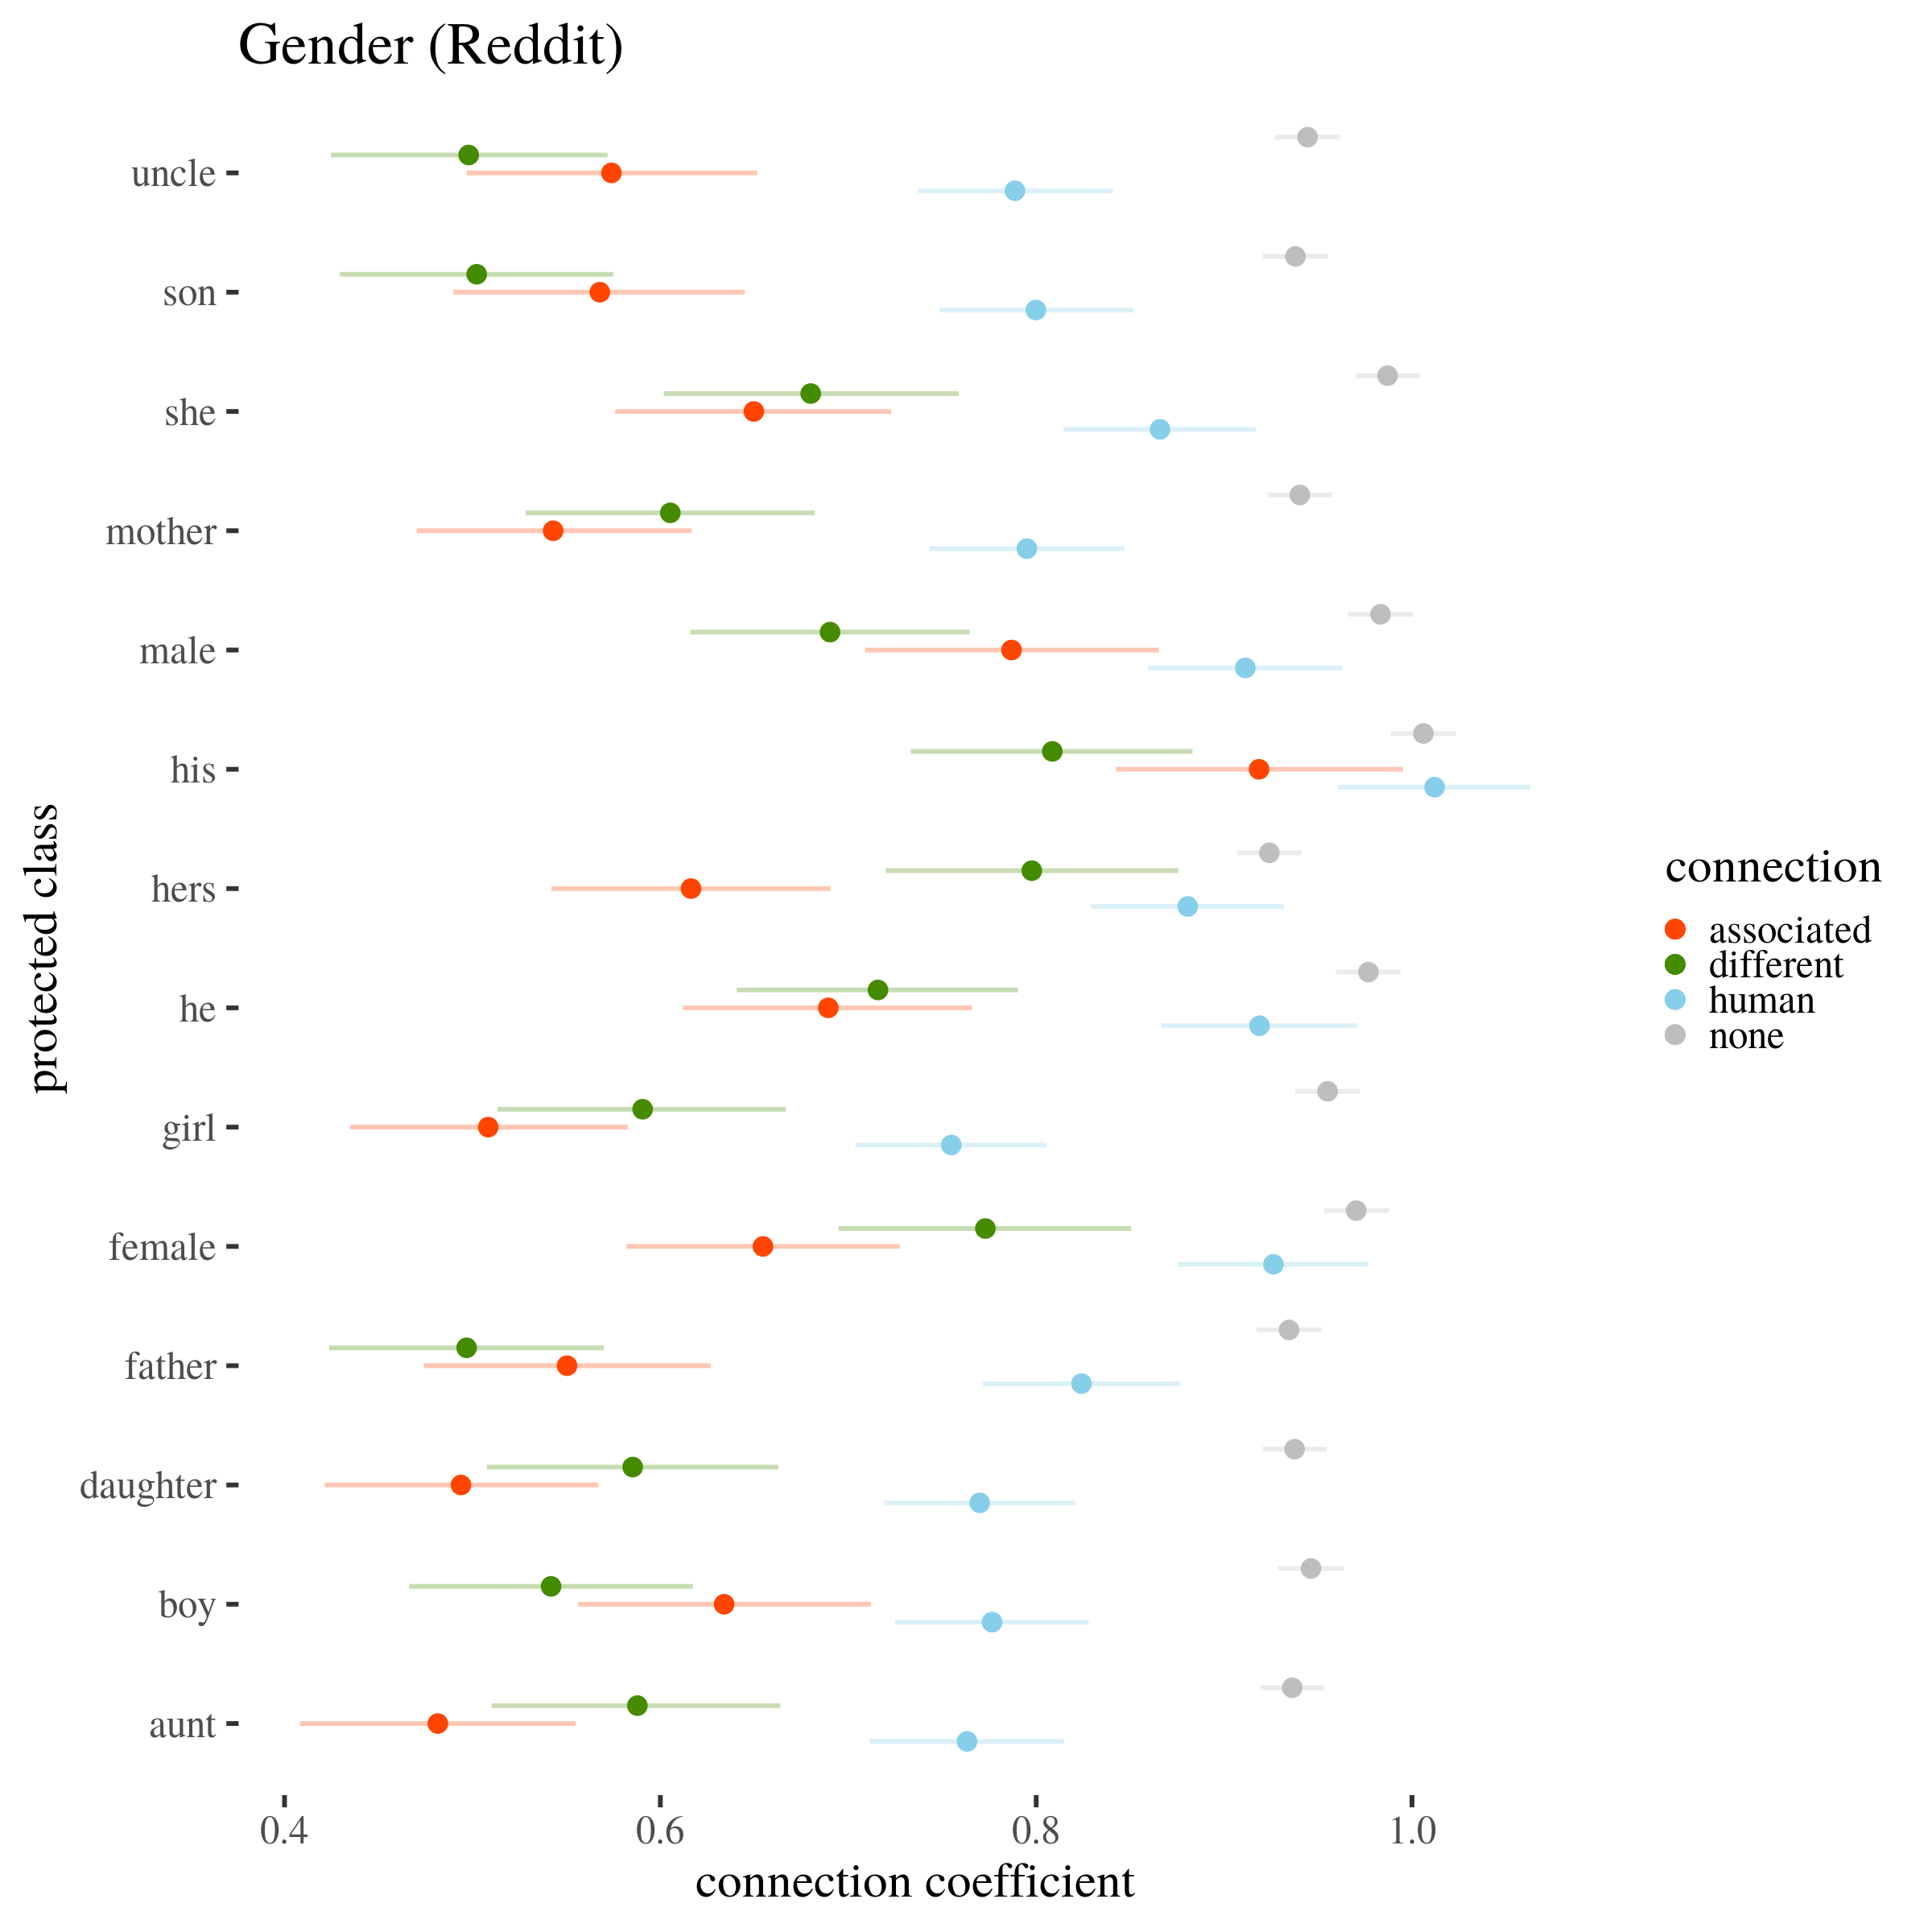
\includegraphics[width=14cm]{../images/visGenderReddit.png}

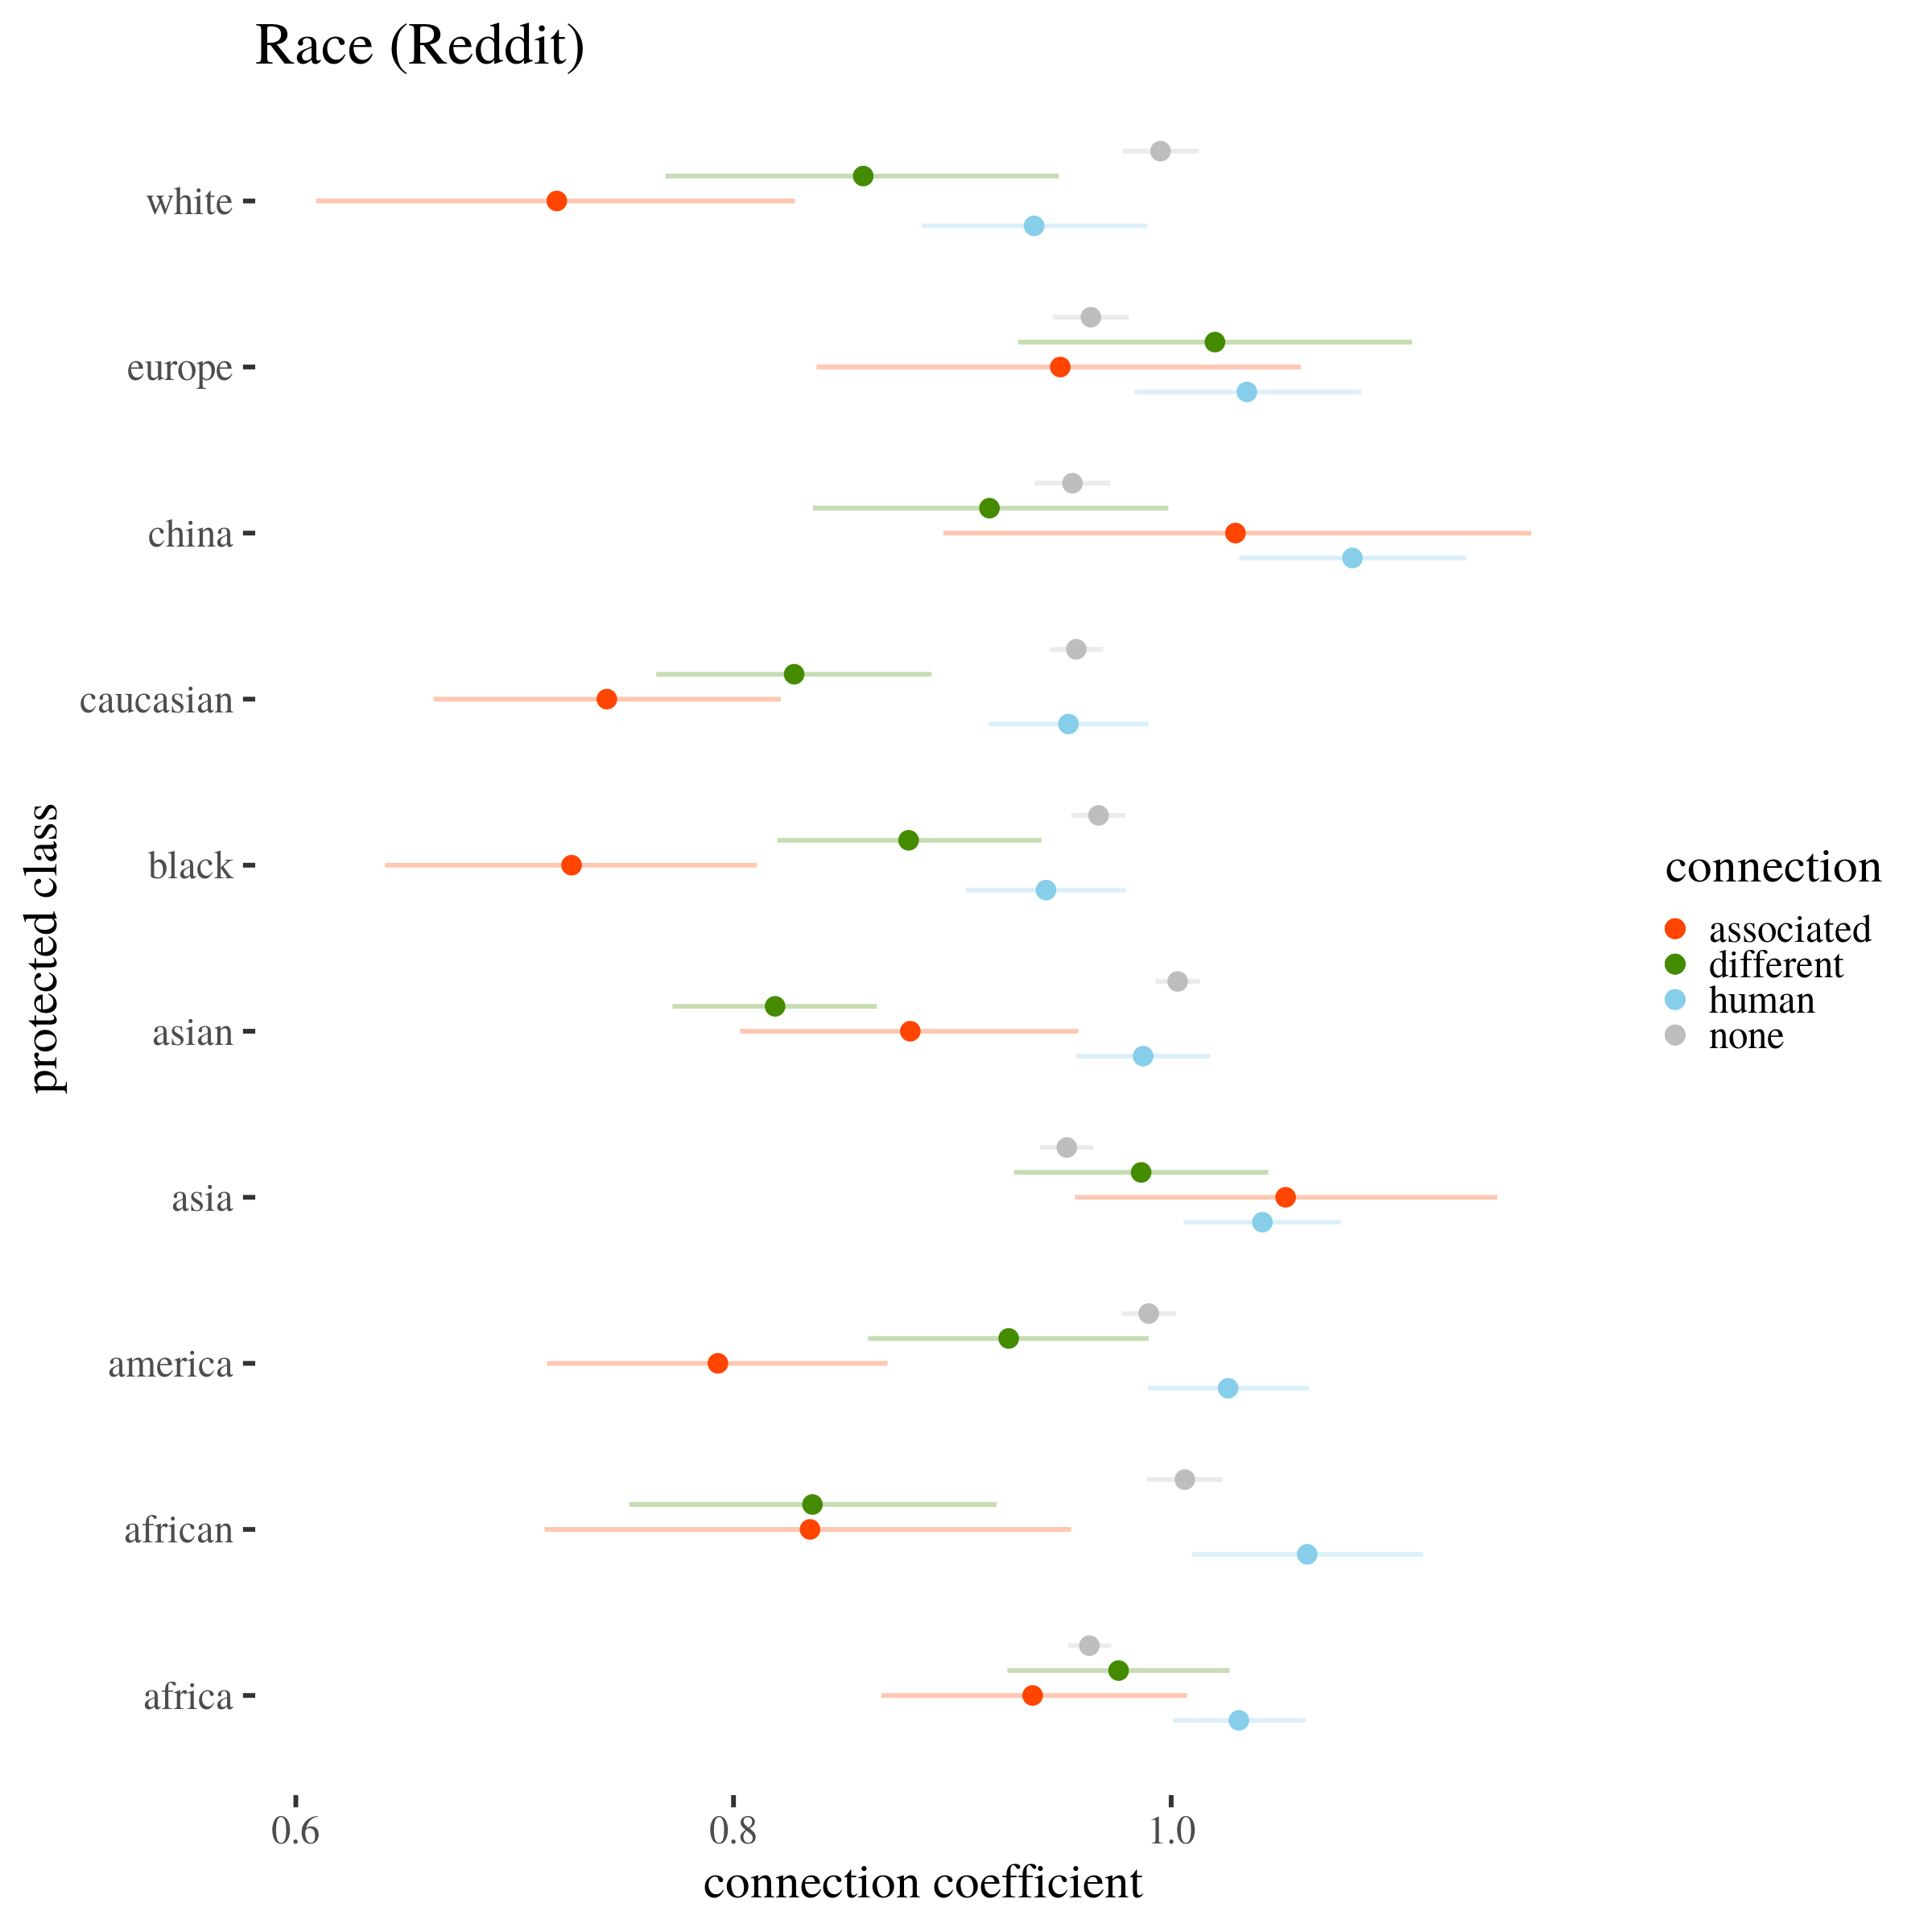
\includegraphics[width=14cm]{../images/visRaceReddit.png}

We first encountered the GoogleNews word embedding model in \protect\hyperlink{ref-Bolukbasi2016Man}{Bolukbasi, Chang, Zou, Saligrama, \& Kalai} (\protect\hyperlink{ref-Bolukbasi2016Man}{2016}). They use it for their calculations as written in \href{https://github.com/tolga-b/debiaswe}{Tolga Bolukbasi code}\footnote{\url{https://github.com/tolga-b/debiaswe}}. We decided to compare the results obtained with the use of Reddit L2 model and the ones that we got by GoogleNews model. The details of the model can be found here \href{https://code.google.com/archive/p/word2vec/}{Google News model}. One of the main differences between the models is that Reddit word embeggings have 50 dimensions and GoogleNews word embeddings have 300 dimensions. As the dimension increases, the vectors can capture much more information, but this is not always the case. According to some researchers, the amount of dimensions should be chosen by taking into account the type of corpus and its features. In our case both Reddit and GoogleNews models are already trained and ready to use so we do not analyse further the choice of their hyperparameters.

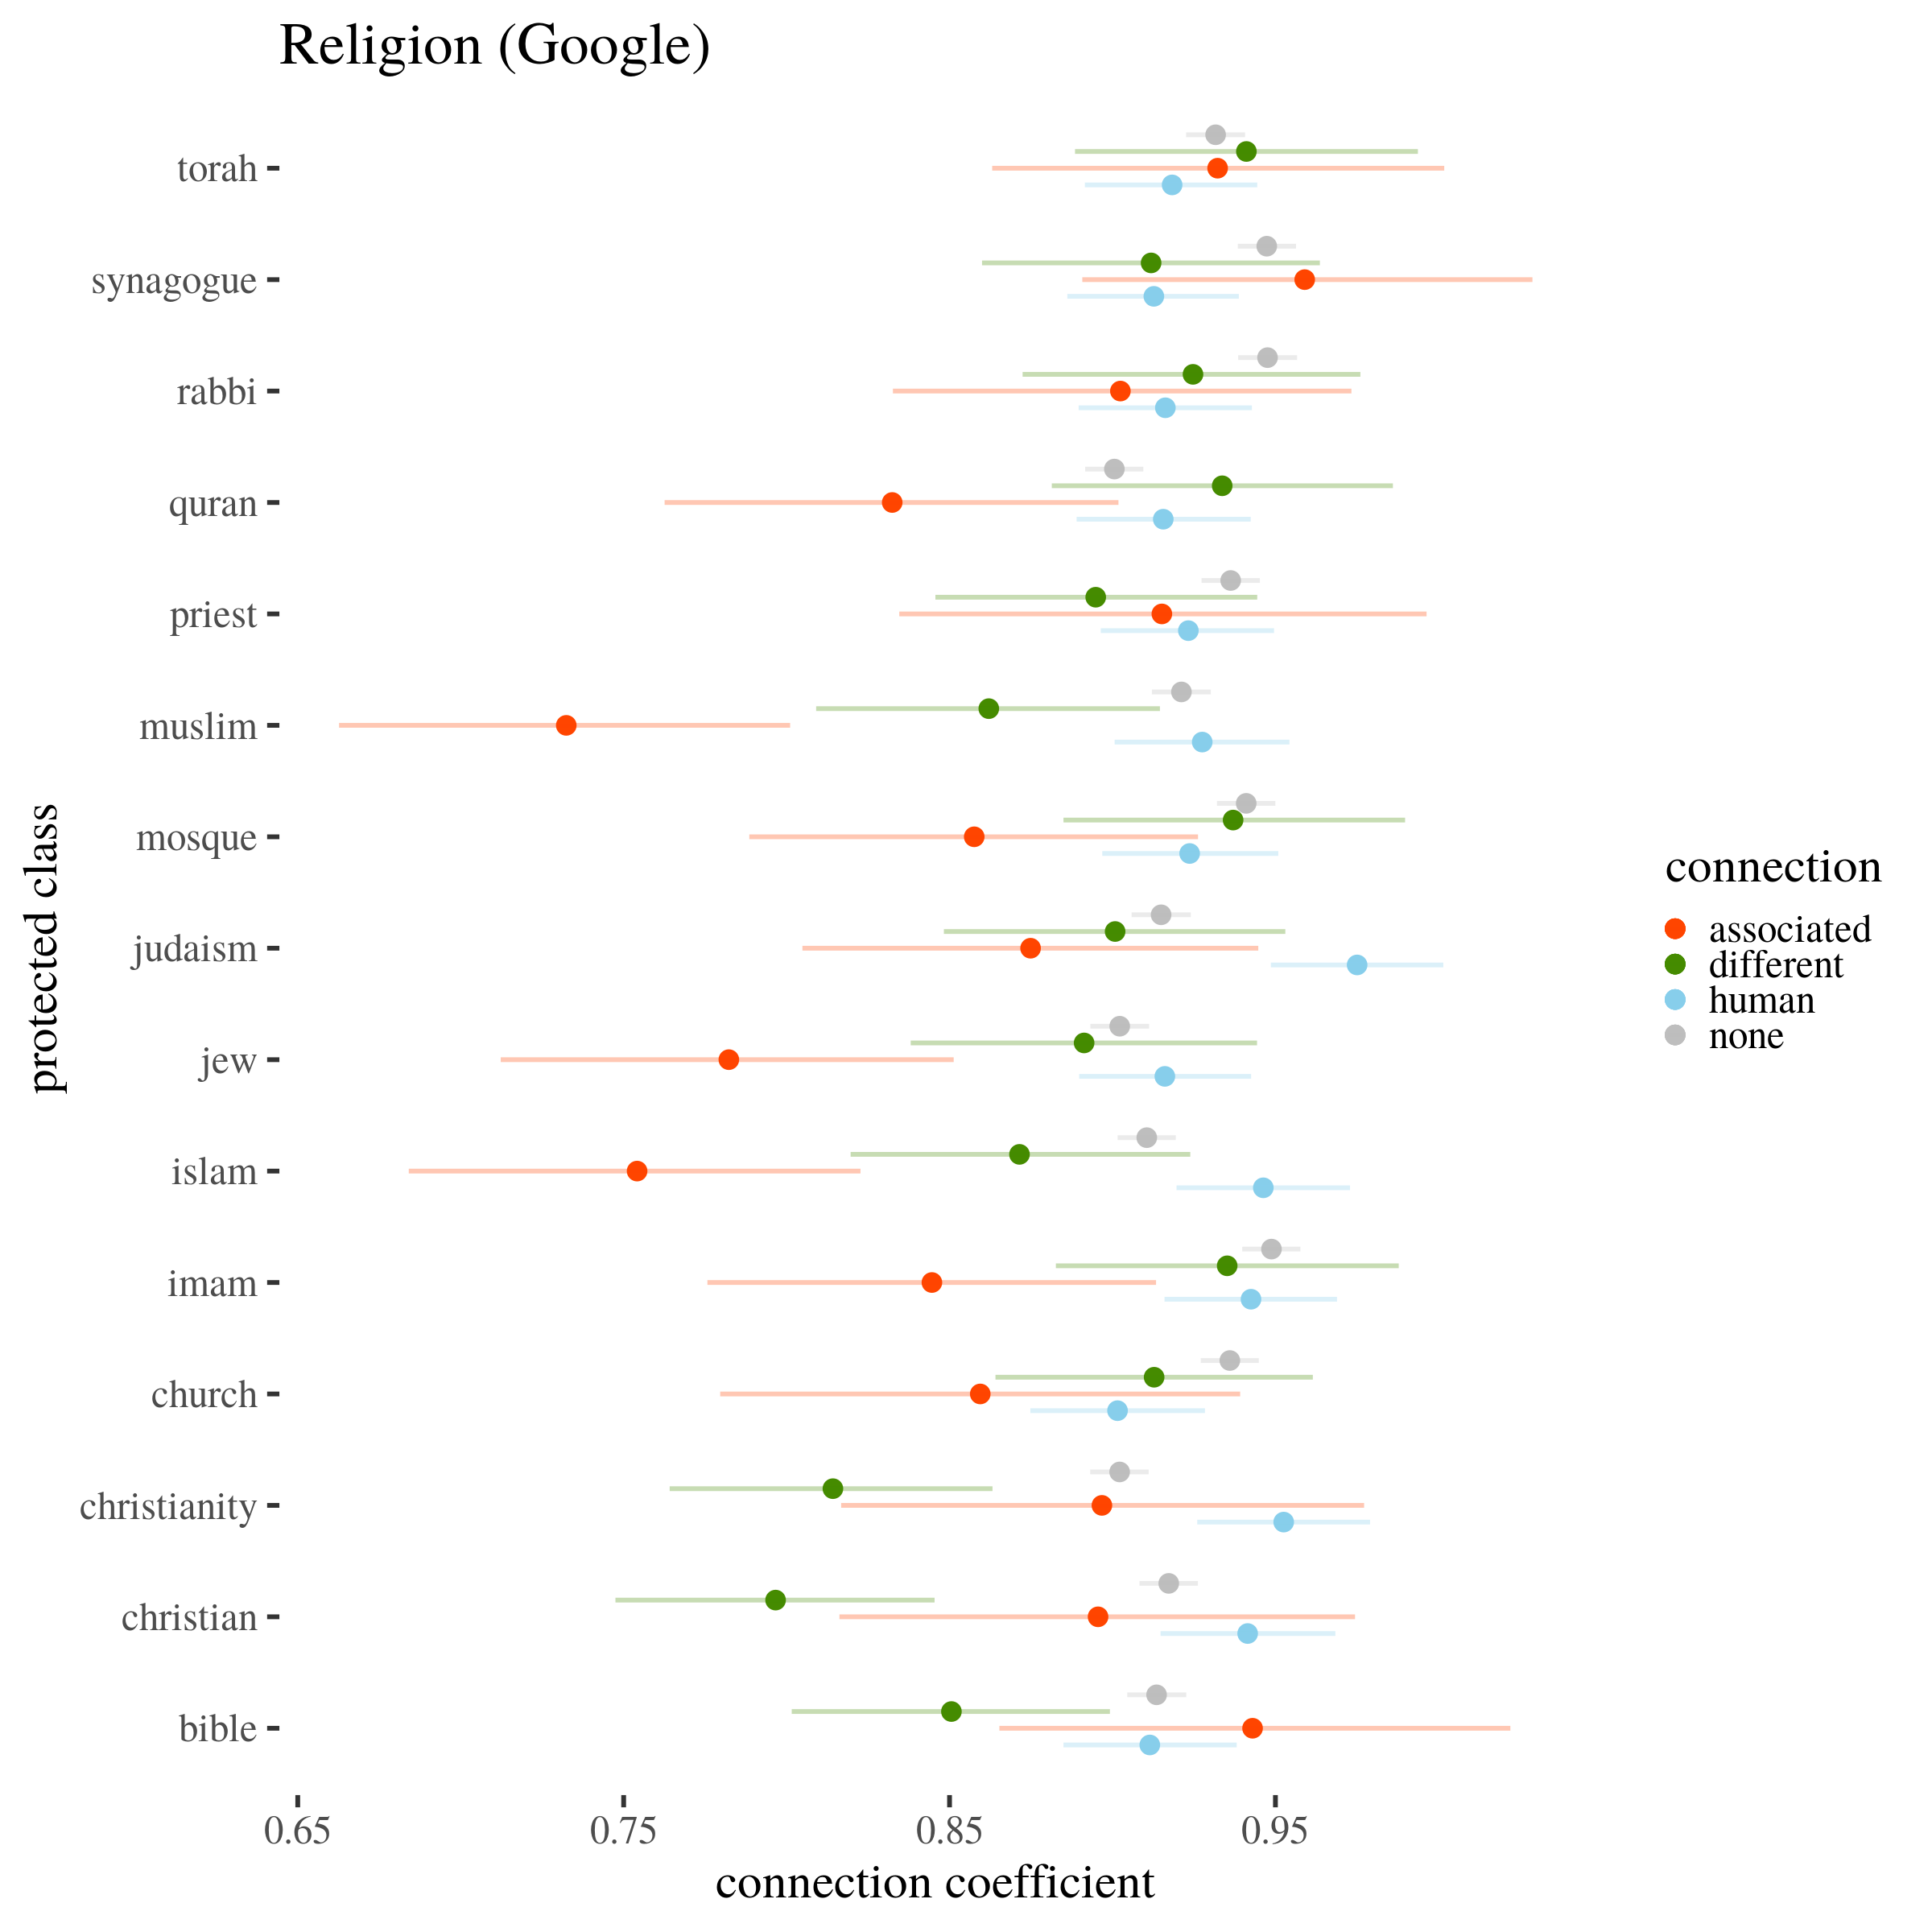
\includegraphics[width=14cm]{../images/visReligionGoogle.png}

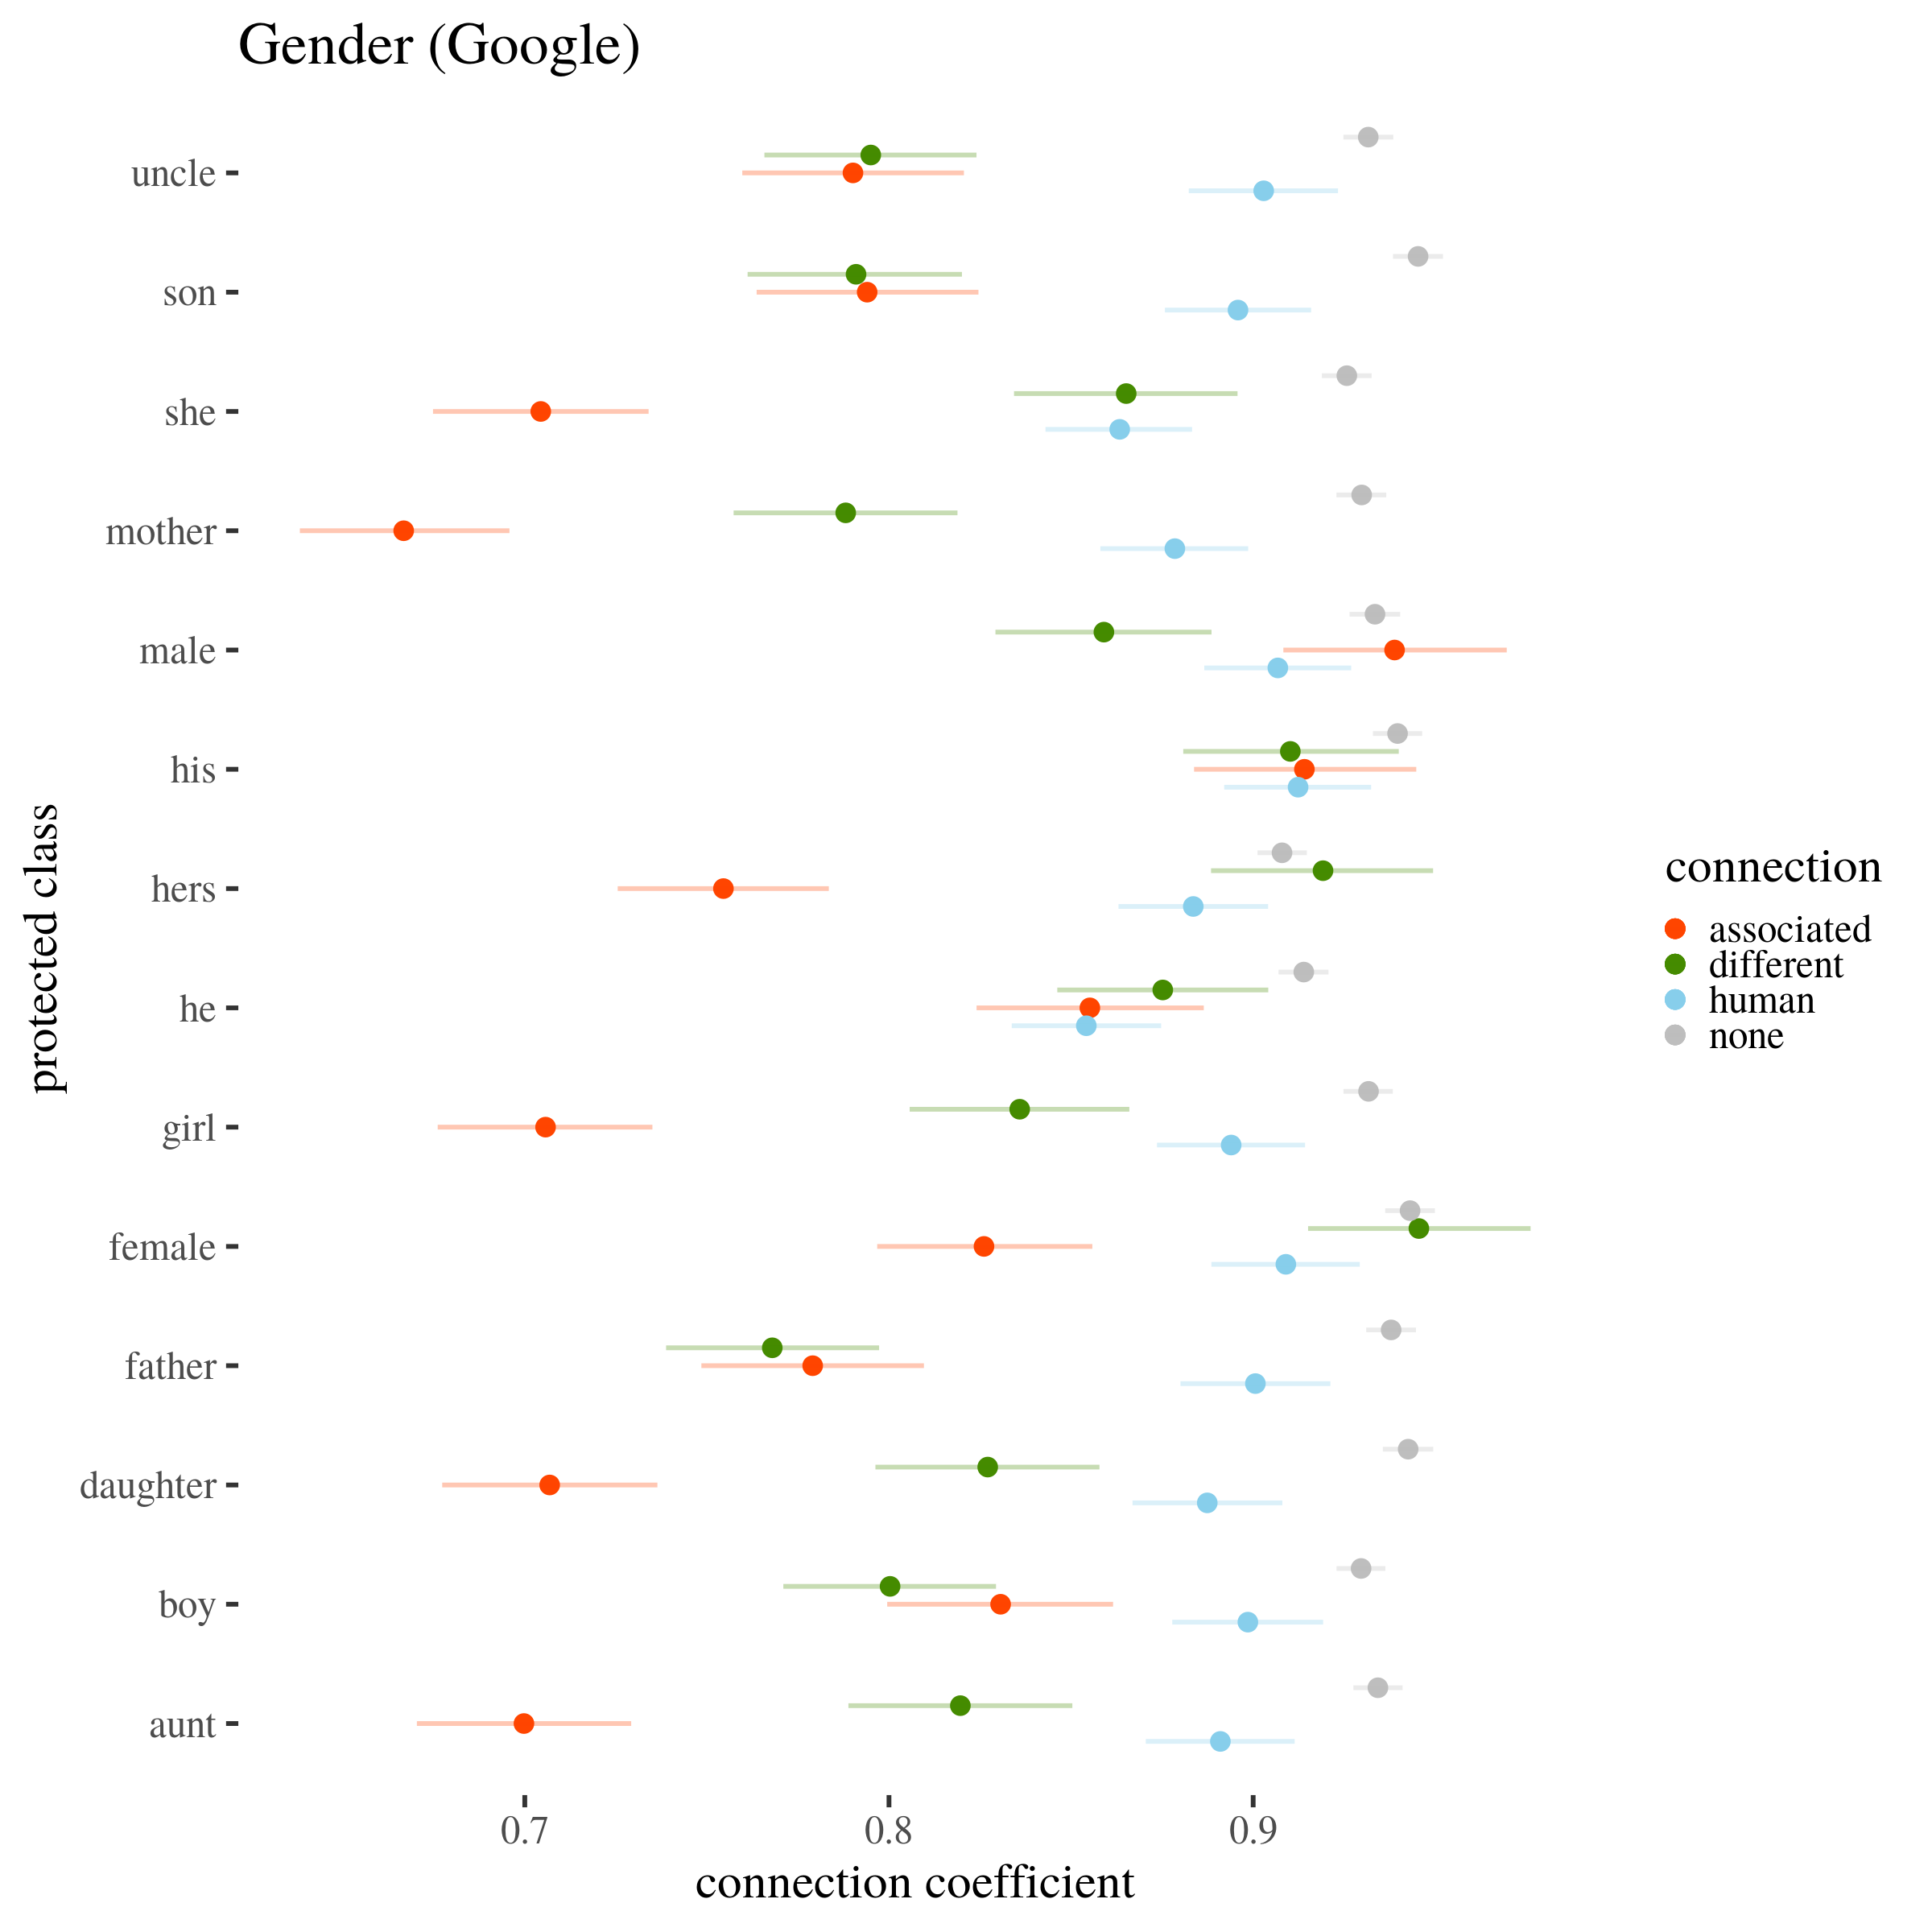
\includegraphics[width=14cm]{../images/visGenderGoogle.png}

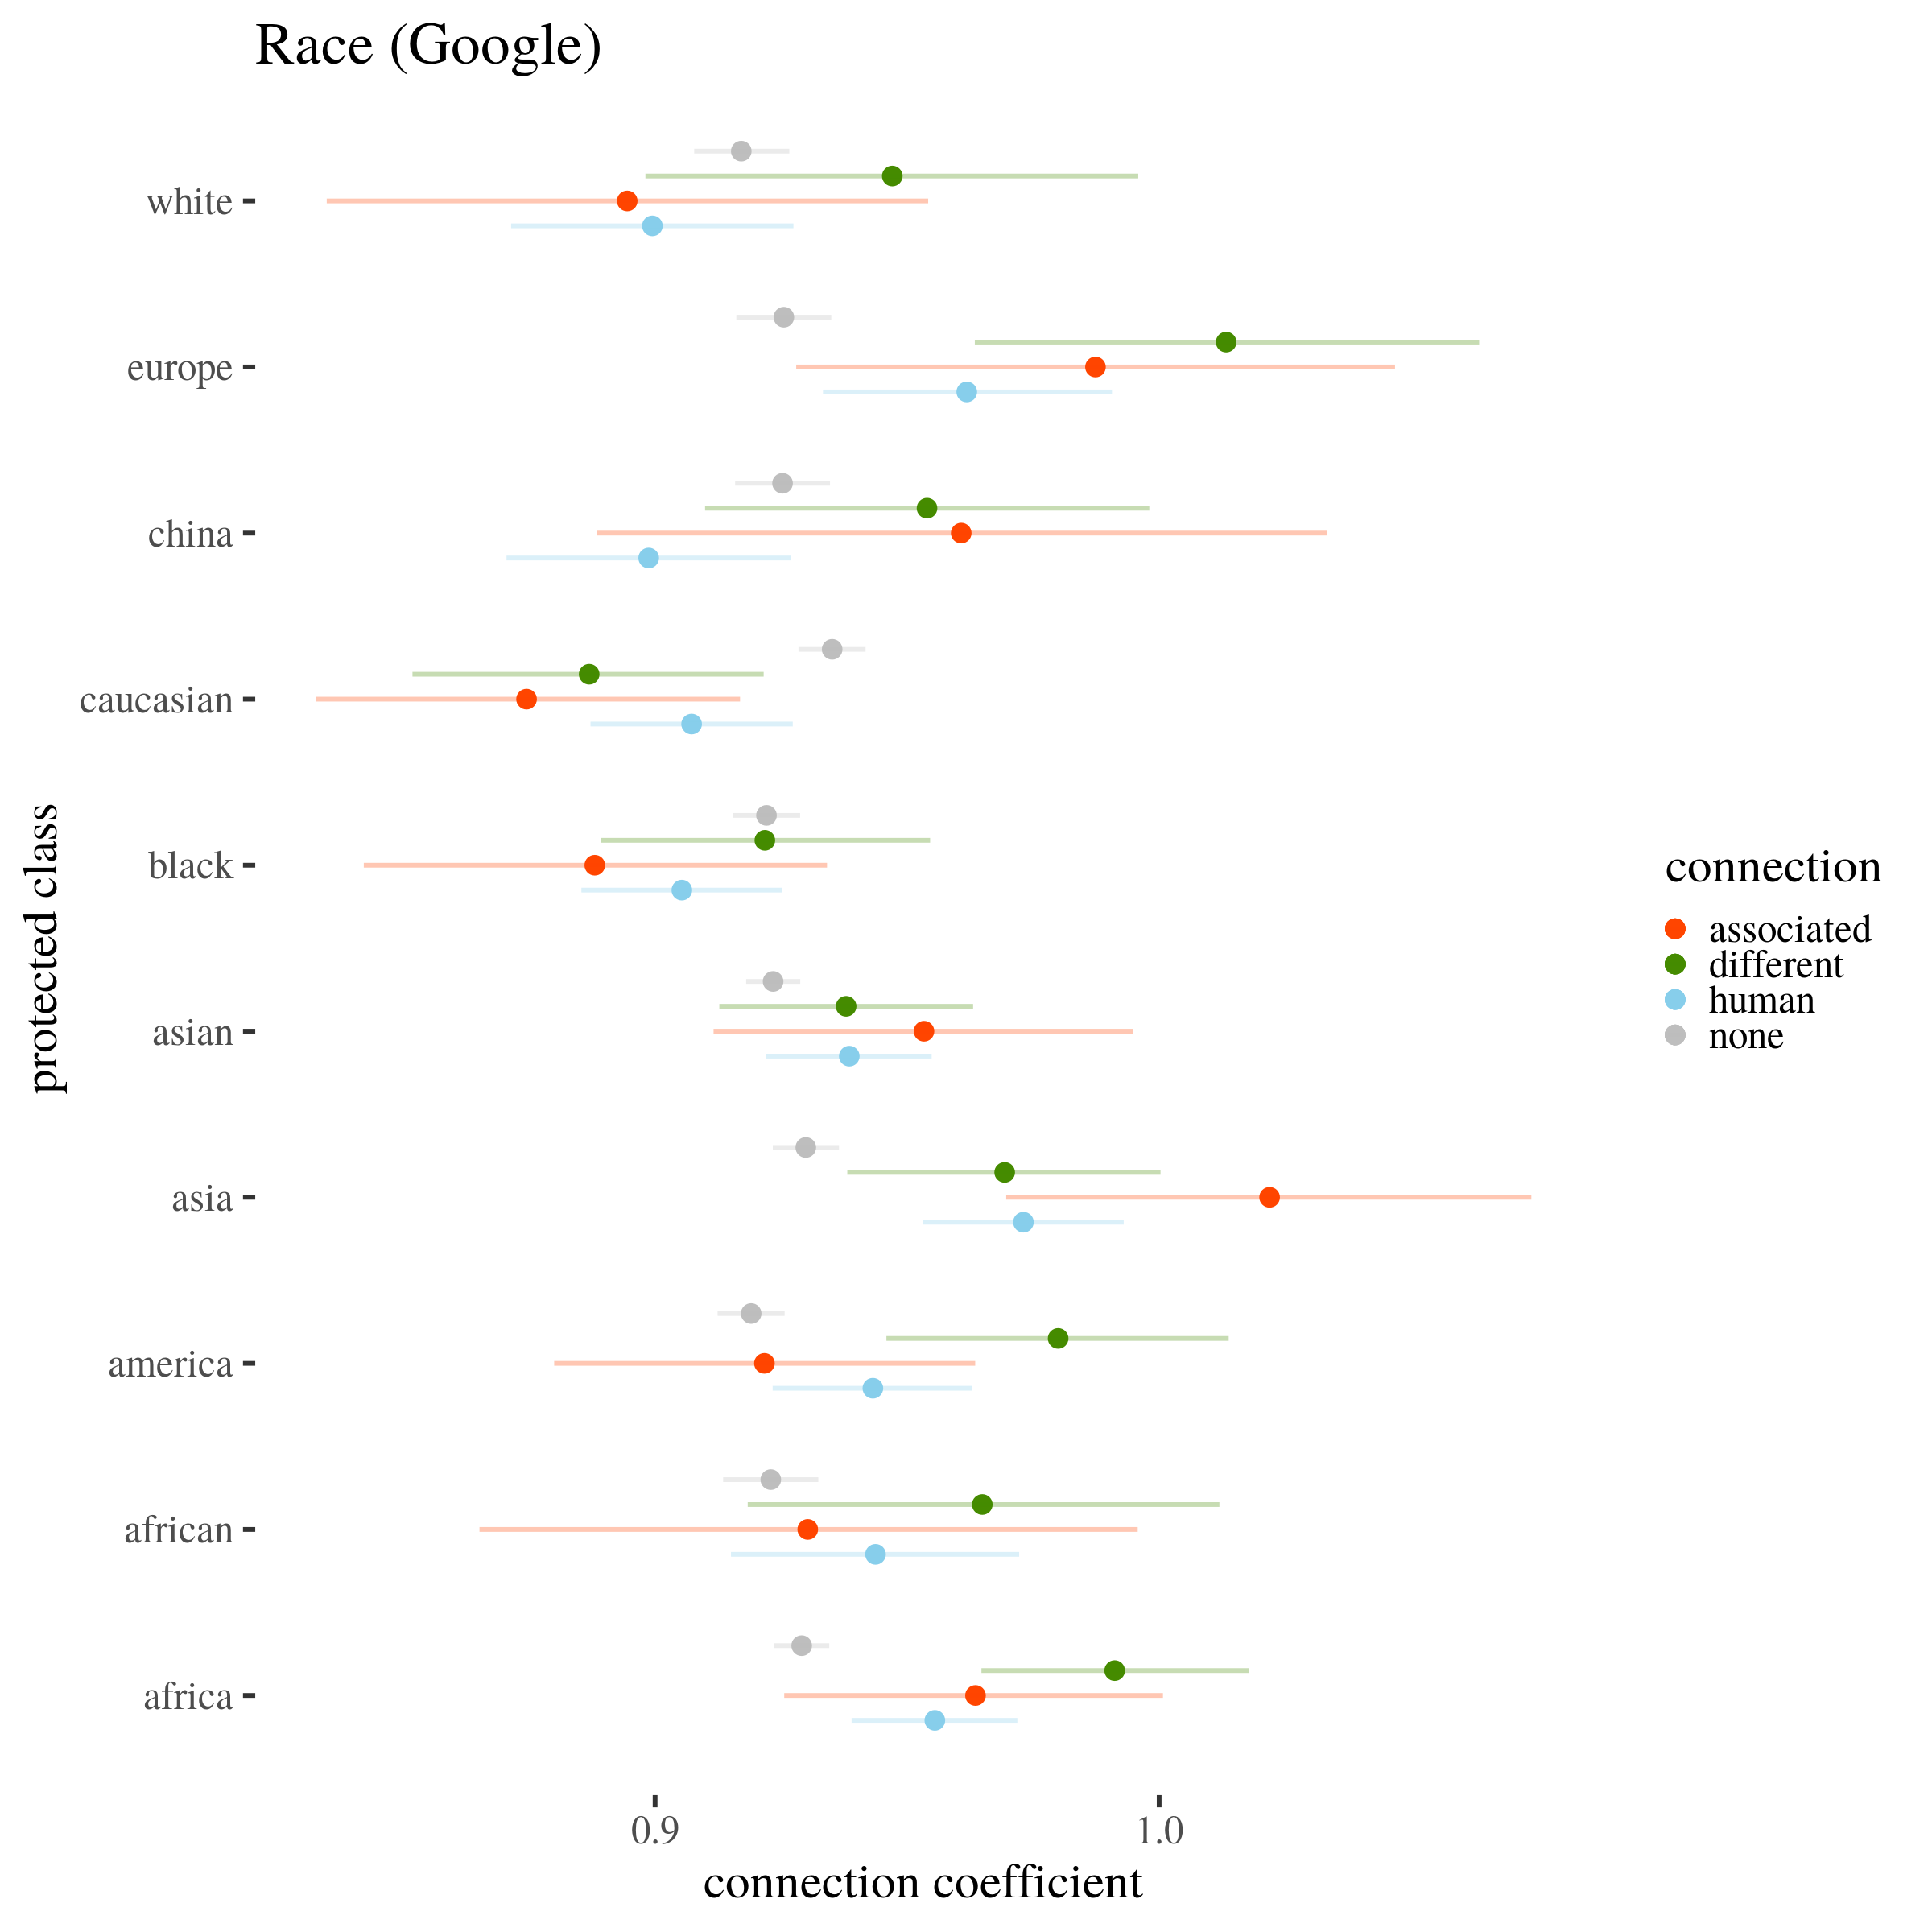
\includegraphics[width=14cm]{../images/visRaceGoogle.png}

We leave a discussion of these results for later, for now let us also inspect the impact of debiasing.

\hypertarget{the-role-of-debiasing}{%
\chapter{The role of debiasing}\label{the-role-of-debiasing}}

We also applied to the word embeddings hard debiasing method found in \protect\hyperlink{ref-Manzini2019blackToCriminal}{Manzini, Lim, Tsvetkov, \& Black} (\protect\hyperlink{ref-Manzini2019blackToCriminal}{2019}). As it was mentioned before, debiasing consists of two components: identifying the bias subspace and then removing this vector subspace from the chosen embeddings. The aim is to increase the cosine distance between protected words and the set of attributes.
After debiasing the Reddit word embeddings we calculated the cosine distance again to see if there are any significant changes in terms of the similarity between protected words and the attributes.

\hypertarget{dataset-level-coefficients-after-debiasing}{%
\section{Dataset-level coefficients after debiasing}\label{dataset-level-coefficients-after-debiasing}}

First, let's look at coefficient estimated for the whole datasets, as compared to their estimation prior to debiasing. One may observe very slight changes in the estimated coefficients. It seems that in religion dataset the changes are the most significant as the mean moves towards zero which stands for no similarity between words.

\begin{center}
\begin{figure}[!htb]\centering
   \begin{minipage}{0.55\textwidth}
  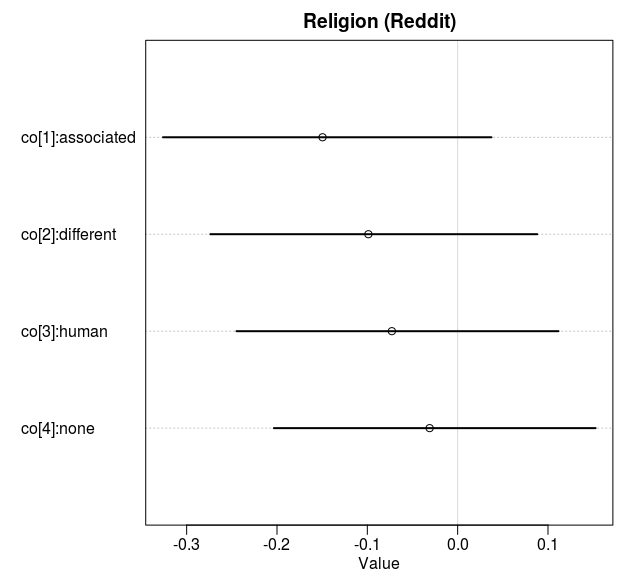
\includegraphics[width=7cm]{../images/religionCoeffs.jpeg}
   \end{minipage}
   \begin {minipage}{0.43\textwidth}
    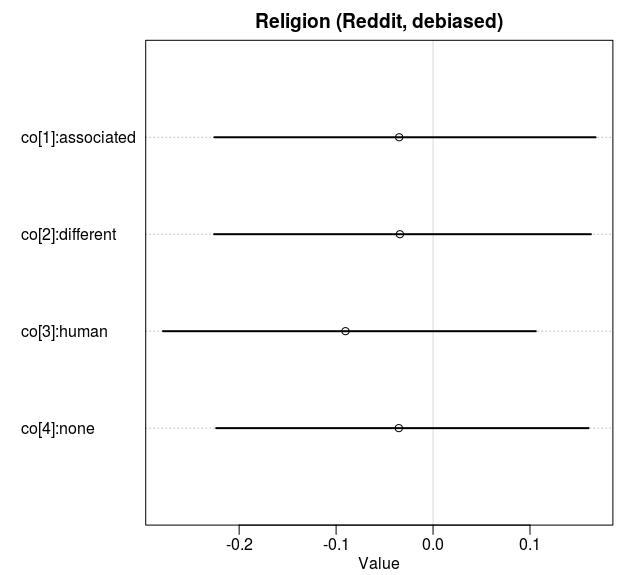
\includegraphics[width=7cm]{../images/debiasedReligionRedditCoeffs.jpeg}
   \end{minipage}
   
   
  \begin{minipage}{0.55\textwidth}
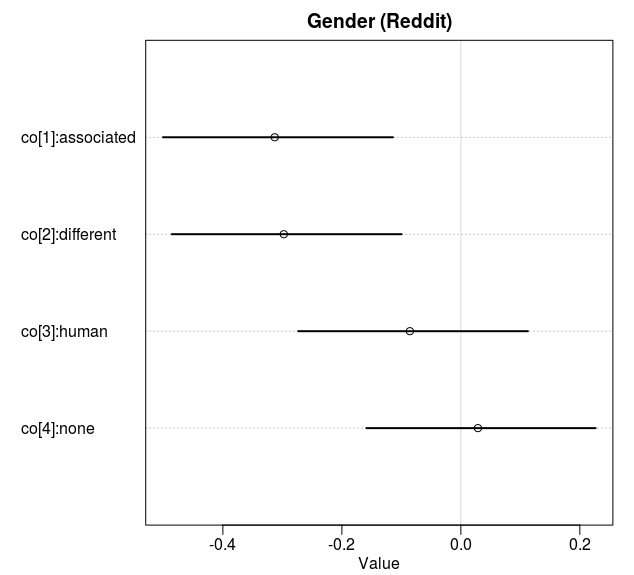
\includegraphics[width=7cm]{../images/genderCoeffs.jpeg}
\end{minipage}
   \begin {minipage}{0.43\textwidth}
    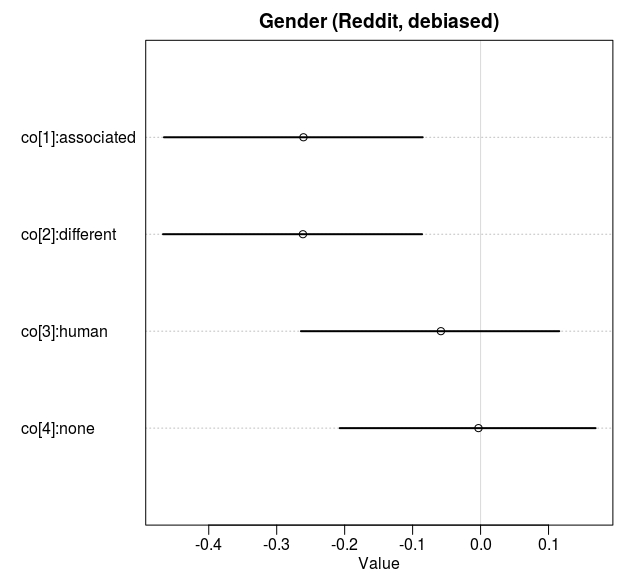
\includegraphics[width=7cm]{../images/debiasedGenderRedditCoeffs.jpeg}
   \end{minipage}
   
   
   
   
  \begin{minipage}{0.55\textwidth}
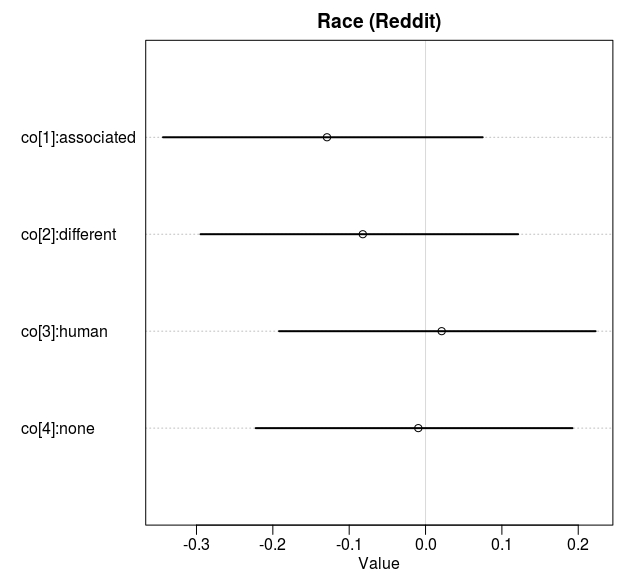
\includegraphics[width=7cm]{../images/raceCoeffs.jpeg}
\end{minipage}
   \begin {minipage}{0.43\textwidth}
    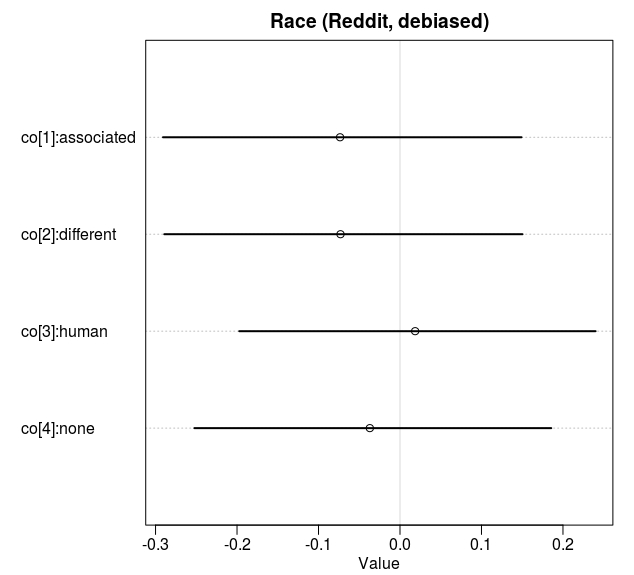
\includegraphics[width=7cm]{../images/debiasedRaceRedditCoeffs.jpeg}
   \end{minipage}
\end{figure}

\end{center}

\hypertarget{protected-classes-after-debiasing}{%
\section{Protected classes after debiasing}\label{protected-classes-after-debiasing}}

Now, perhaps, the effects of debiasing will be better appreciated if we look at the level of protected words. After all, the hope is, the situation of extremely ill-positioned protected words have improved?

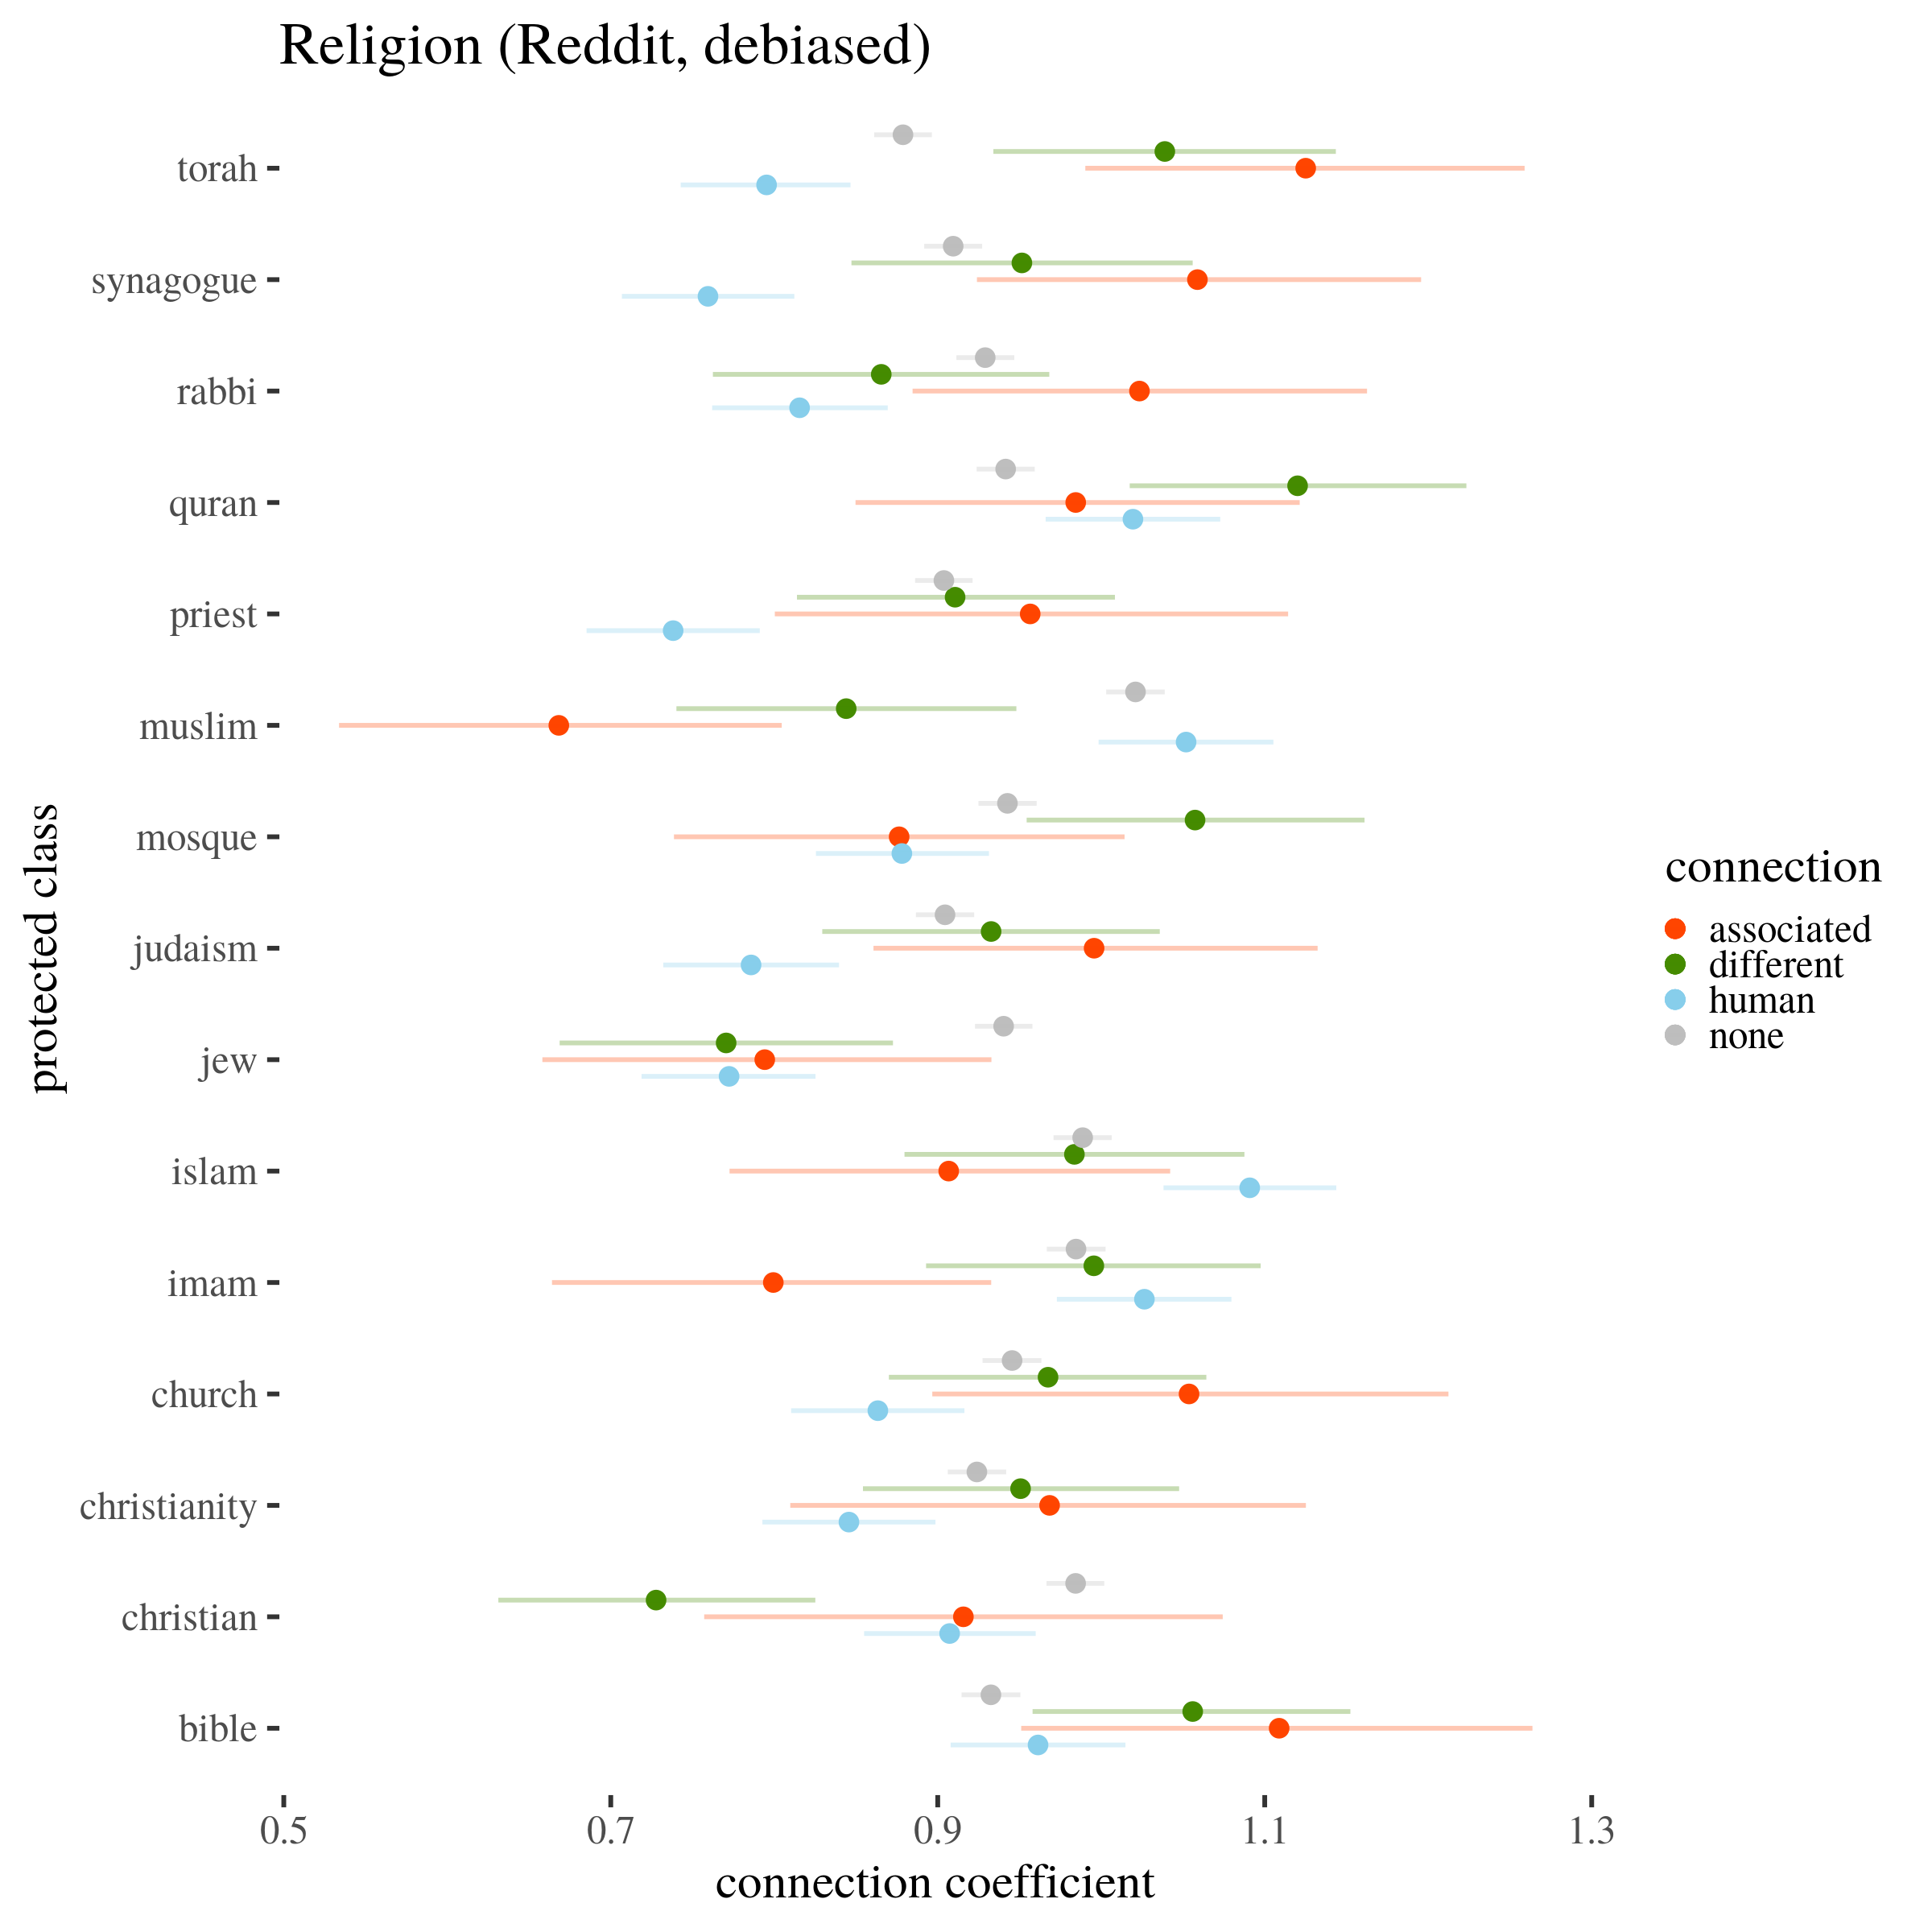
\includegraphics[width=14cm]{../images/visDebReligionReddit.png}

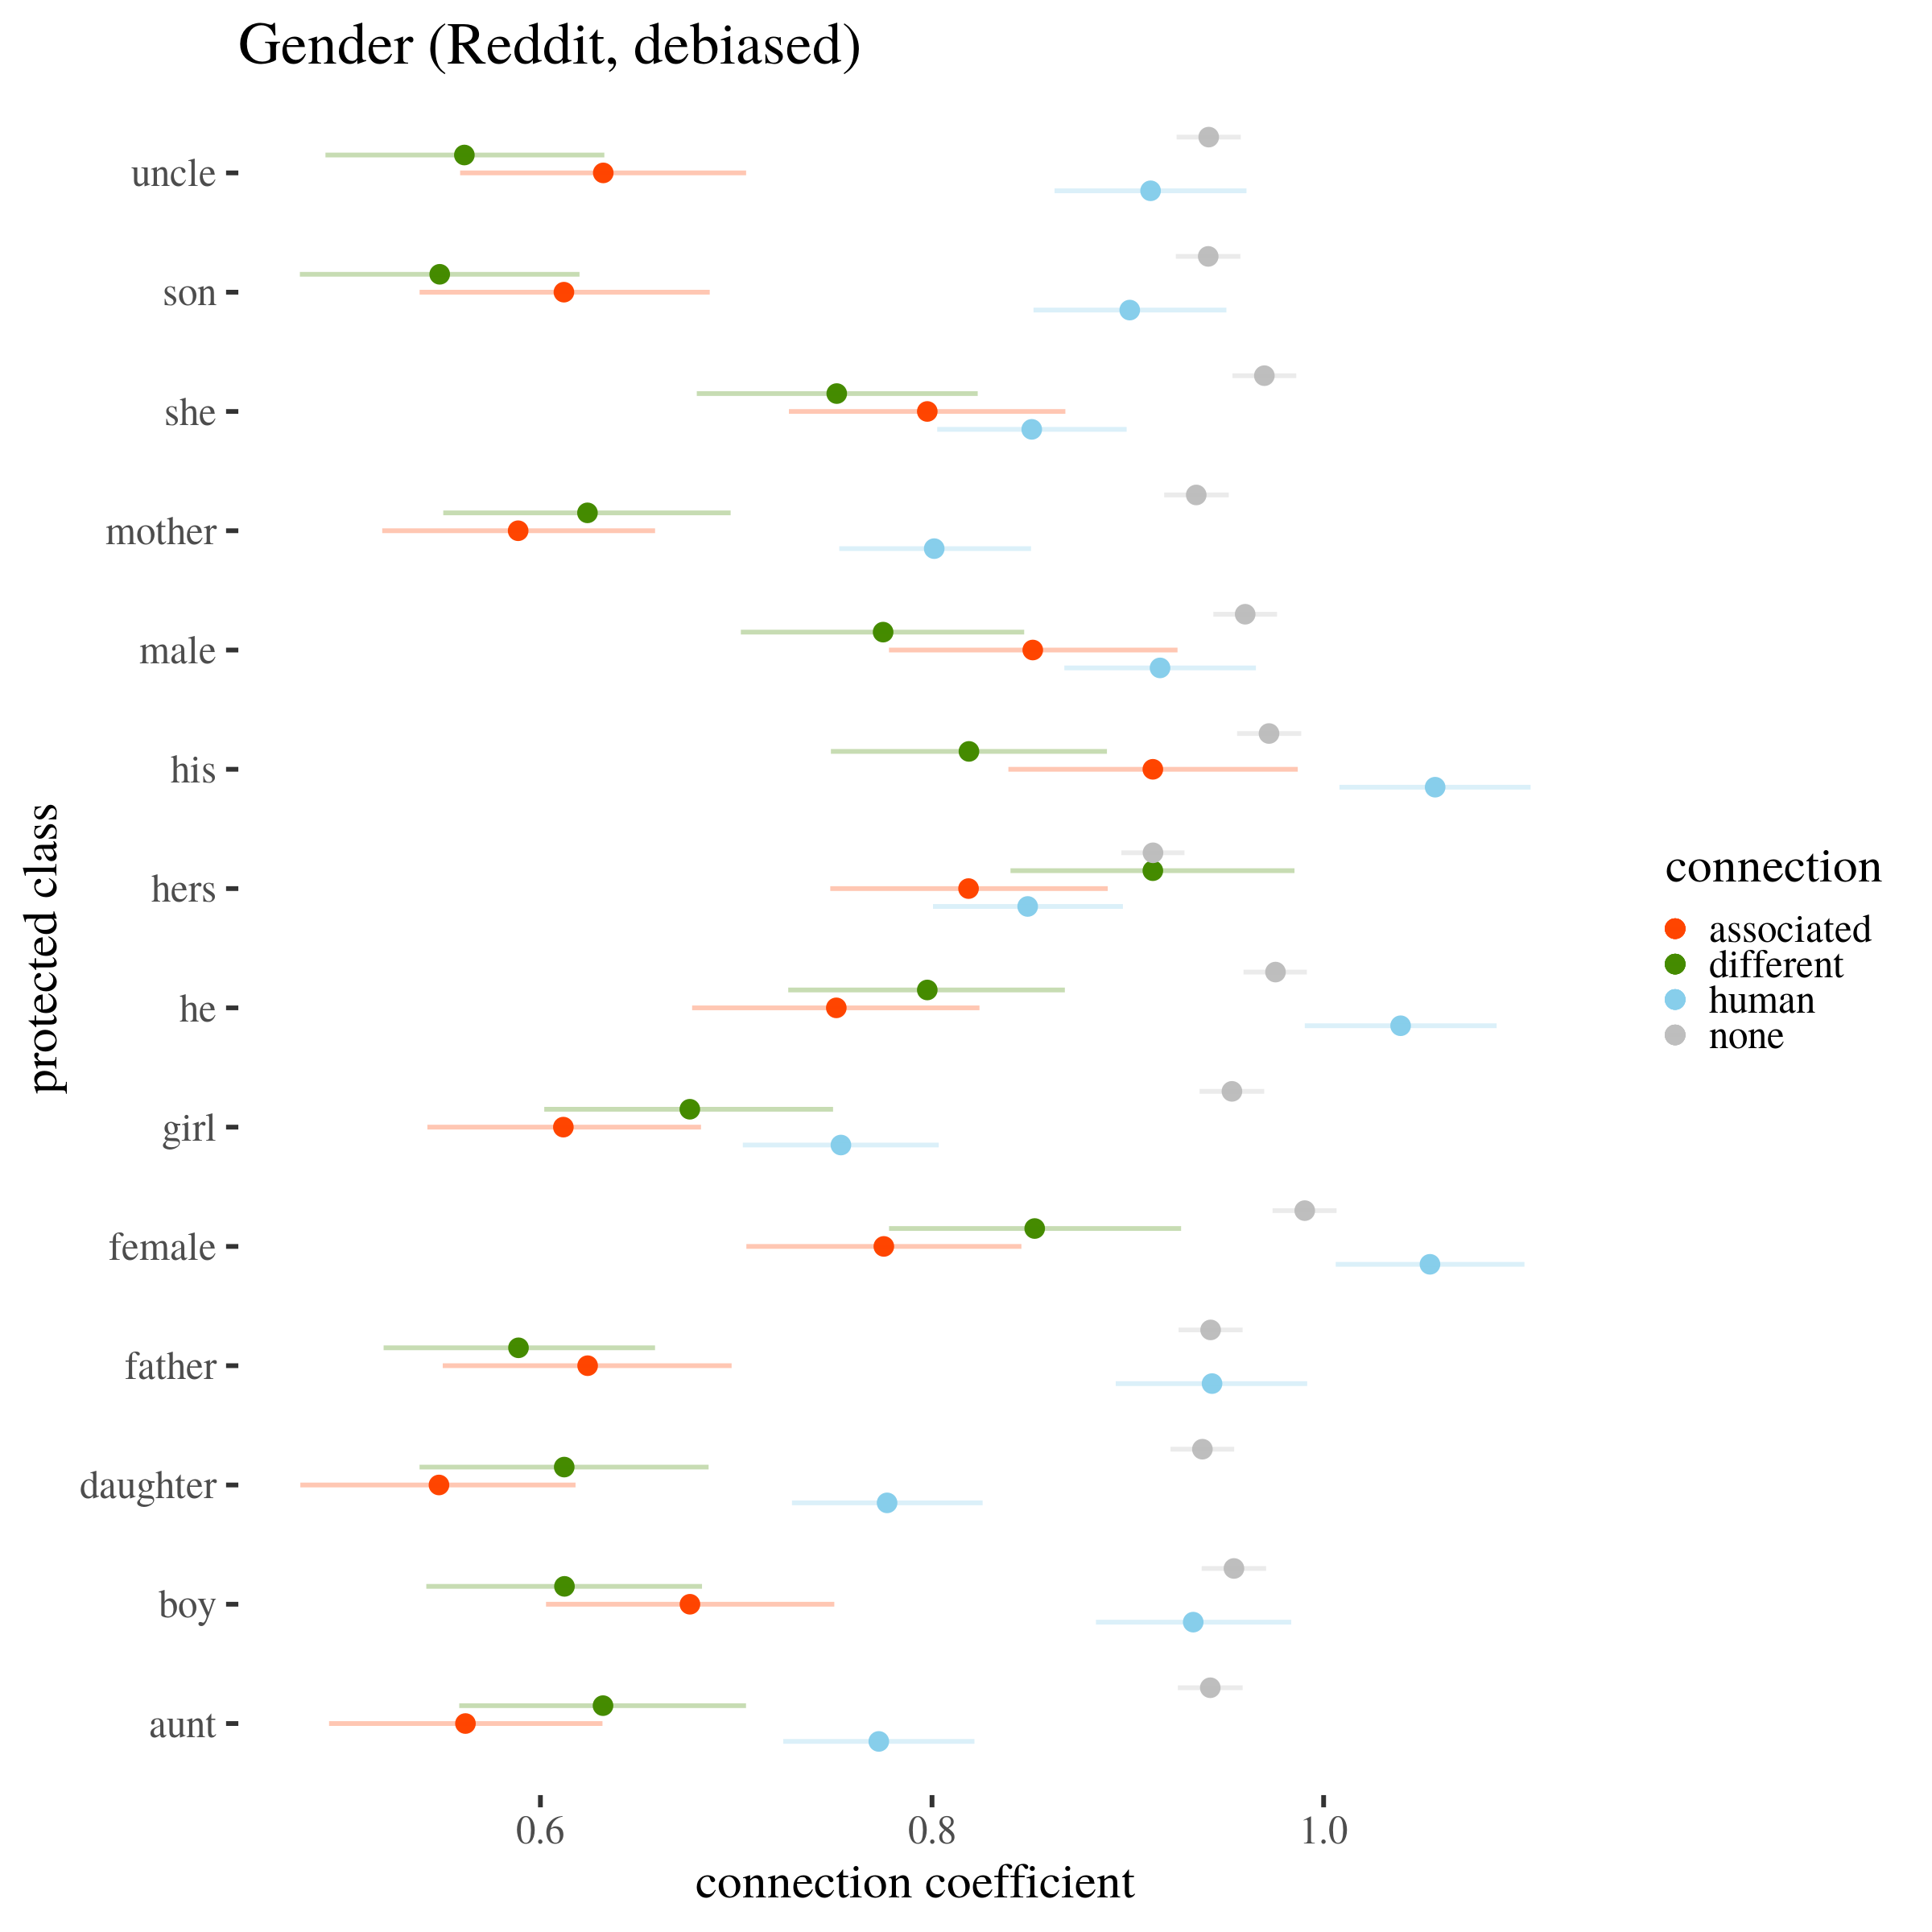
\includegraphics[width=14cm]{../images/visDebGenderReddit.png}

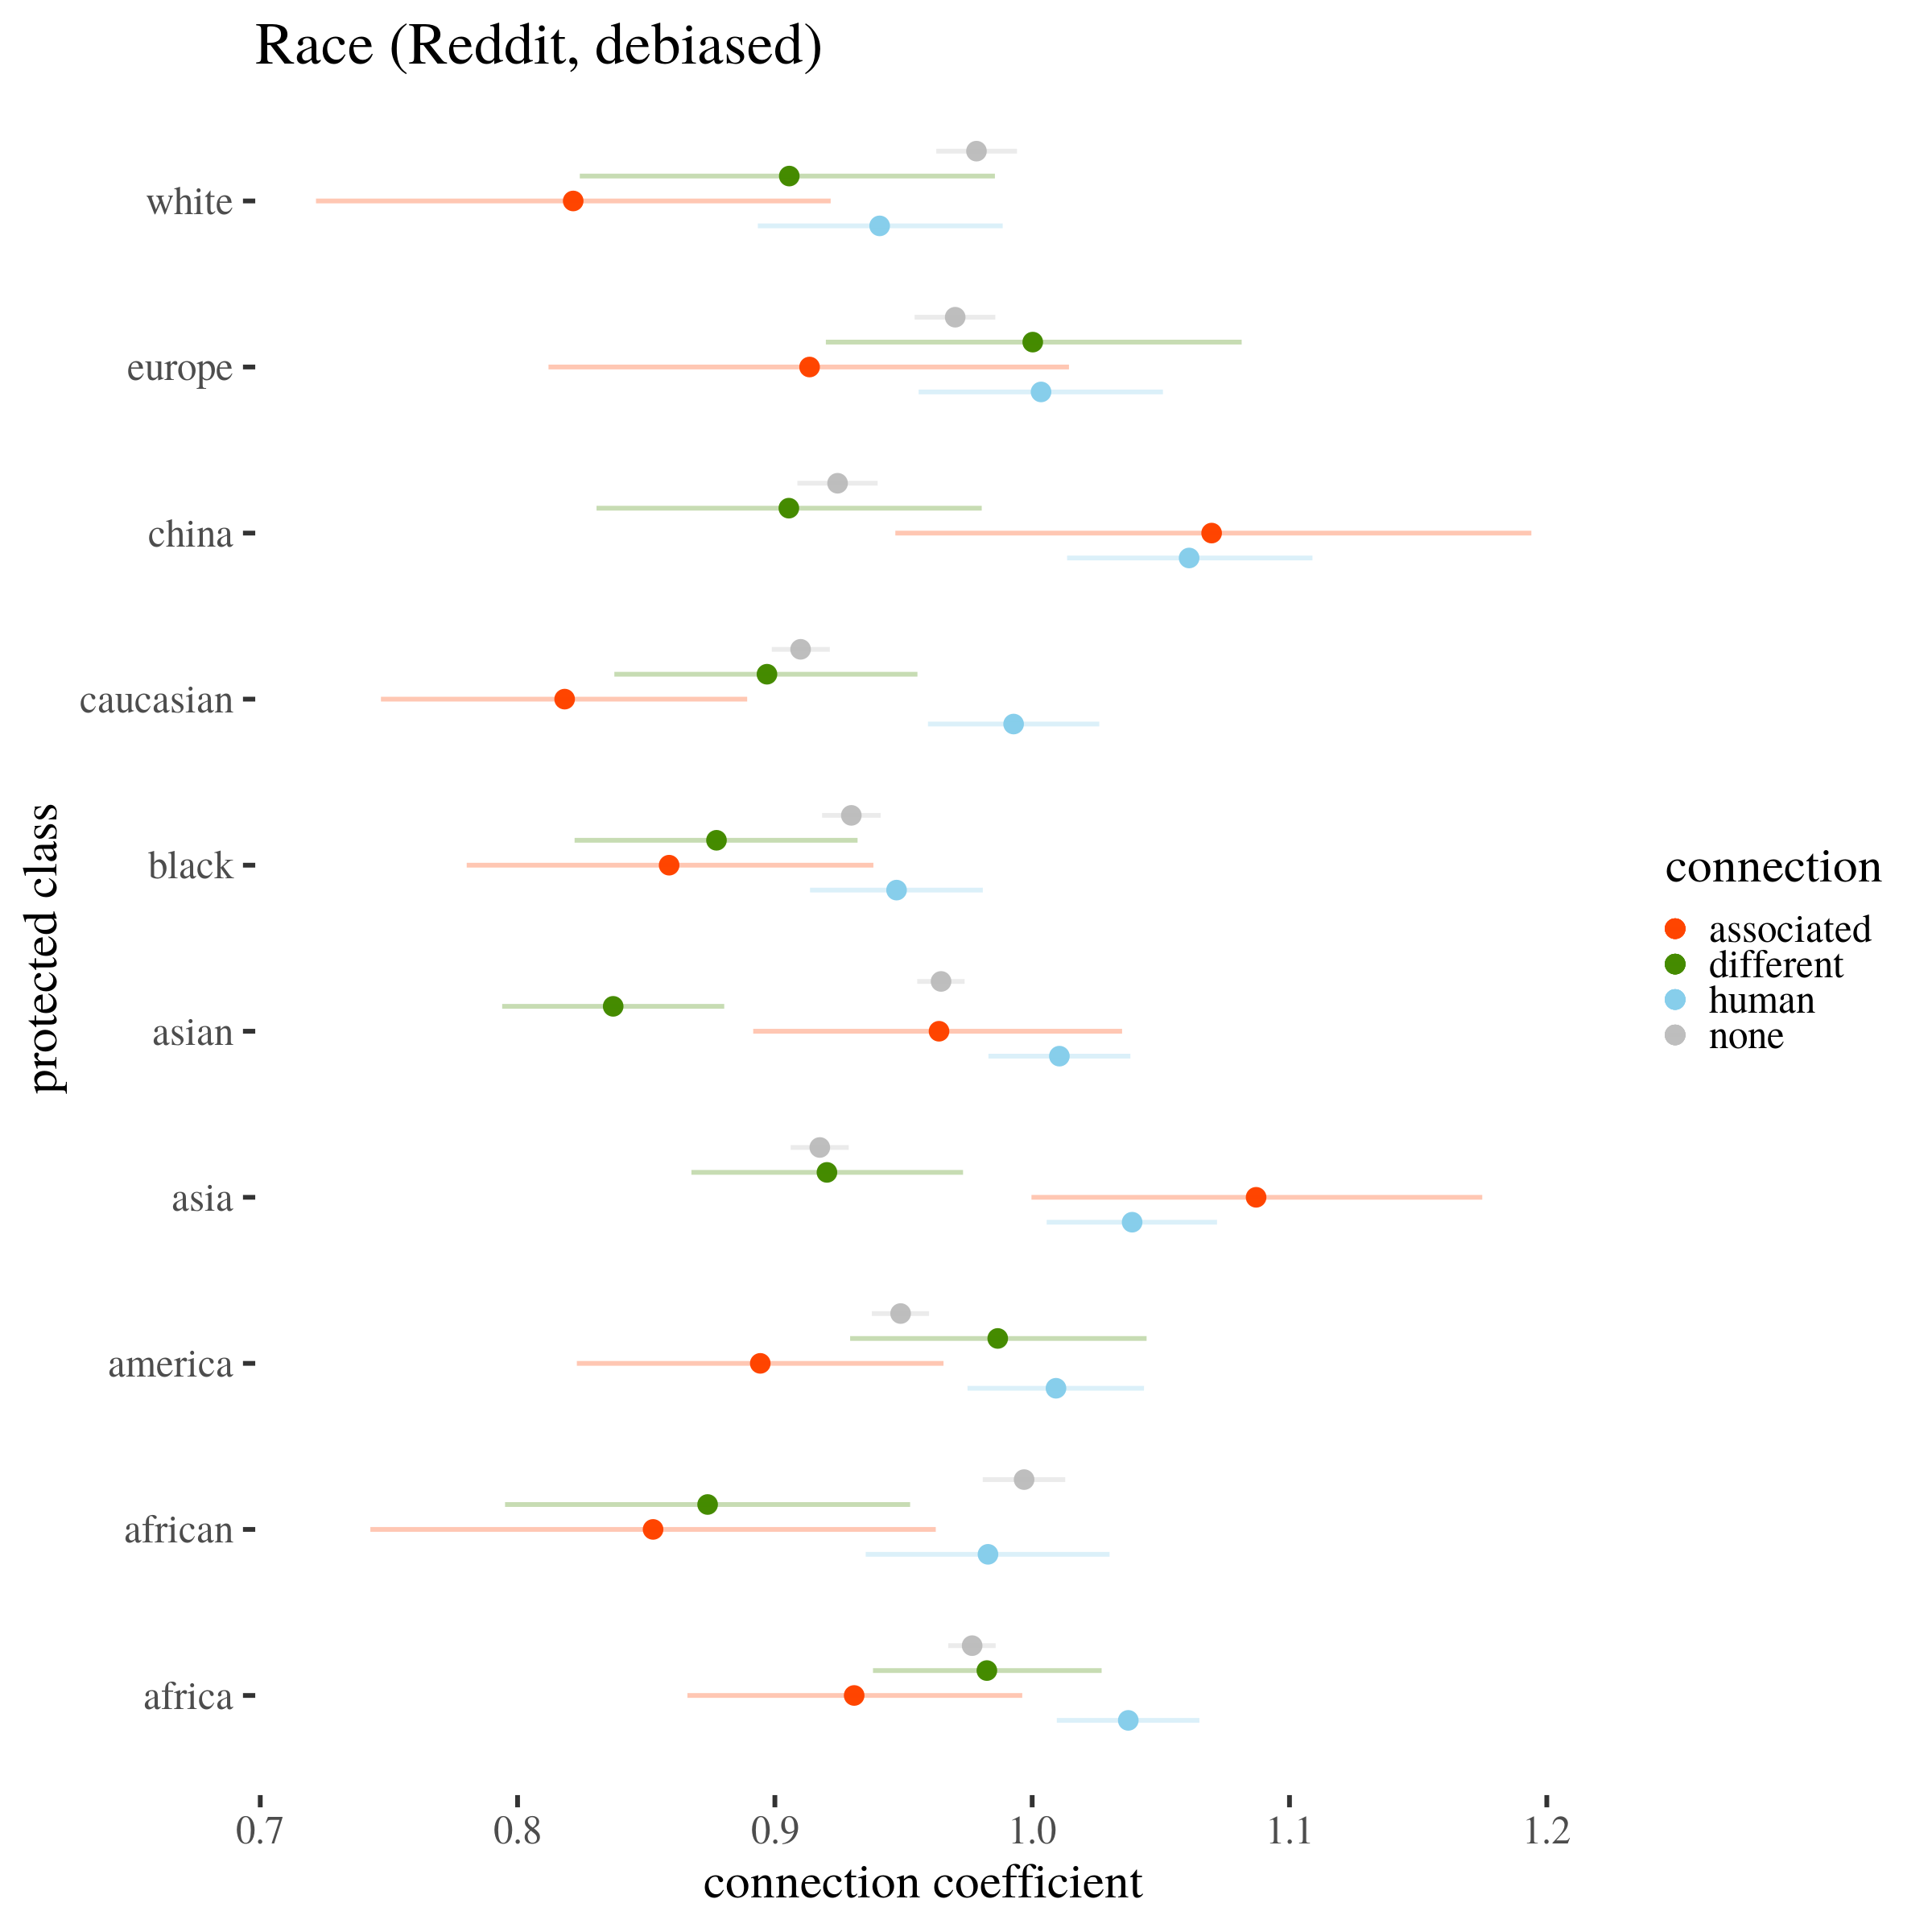
\includegraphics[width=14cm]{../images/visDebRaceReddit.png}

One may notice that in a religion data set most of the distances for \texttt{associated} words slightly increased. Some of the distances from \texttt{different} class are still smaller than for the \texttt{associated} class. The distances for all classes seem in most cases to cluster together even after debiasing. The reason may be that uncertainty is quite high in \texttt{associated} and \texttt{different} class because the number of samples is so small. Additionally in some cases distances from \texttt{human} class are smaller than for the \texttt{assosiated} class which also makes it less clear how to interpret the results, if the distances are really able to catch the bias presence.

It is worth paying attention to the gender debiased dataset. The change is really minor, still with zero out of the HPDI range. The \texttt{different} attributes still have high similarity value. It seems that the distances for gender protected words are still clustered together which suggests that this method is unable to catch the complex bias presence. One could conclude that co-occurrence of certain terms does not always mean direct connection in terms of terms associations. The fact that some of stereotypically associated with female attributes still have high similarity with male protected words suggest that other techniques should be applied to detect and remove the bias.

At the same time, there is a small improvement in race dataset. In some cases the distances just cluster together. In general distances for \texttt{assosiated} class are still higher than those for the rest of classes. One may assume that there reason for so small change is that either the metric does not indicate properly biases or that the issue is more complex and subtracting subspaces is not enough.

\hypertarget{discussion-and-summary}{%
\chapter{Discussion and summary}\label{discussion-and-summary}}

We propose the use of Bayesian methods to measure uncertainty in bias detection. There are a few advantages of this method. One of them is that including uncertainty enables one to directly observe the influence of sample sizes. Analyzing individual words and connection coefficients, one may notice how \texttt{neutral} words have smaller uncertainty intervals and \texttt{different} or \texttt{associated} quite the opposite. One of the reasons for such an outcome is that we used approximately 230 neutral words and only between 11-25 (the number varies from class to class) stereotypical attributes from \protect\hyperlink{ref-Manzini2019blackToCriminal}{Manzini, Lim, Tsvetkov, \& Black} (\protect\hyperlink{ref-Manzini2019blackToCriminal}{2019}) article. In our approach, we also pay attention to the distribution and details regarding anomalous values. With the use of simple visualizations that we introduced before, we were able to indicate suspicious cosine distance values. Additionally, we compare in details how the cosine distance values and uncertainty change after the debiasing. One can investigate then how the individual vectors changed and if it is what was expected. Our analysis with the use of Bayesian method gave us new ideas and hypothesis concerning not only the bias detection method but also the efficiency of debiasing itself.
We created summary tables for each of the datasets: Google word embeddings (Table \ref{tab:dTabG}), Reddit (Table \ref{tab:dTabR}), and Reddit Debiased (Table \ref{tab:dTabRD}).

\vspace{1mm}
\footnotesize
\begin{table}

\caption{\label{tab:dTabG}Overview statistics  (GoogleNews embedding)}
\centering
\resizebox{\linewidth}{!}{
\begin{tabular}[t]{llll}
\toprule
  & Religion (percent) & Gender (percent) & Race (percent)\\
\midrule
A close to N & 66.67 & 14.29 & 80\\
A close to H & 66.67 & 21.43 & 100\\
H closer than A & 20 & 21.43 & 50\\
D similar with A & 93.33 & 42.86 & 100\\
D closer than A & 33.33 & 21.43 & 30\\
General HPDI outside of  0 & no & no & no\\
General D similar to A & slightly not & slightly not & slightly not\\
\bottomrule
\end{tabular}}
\end{table}
\normalsize

\vspace{1mm}
\footnotesize
\begin{table}

\caption{\label{tab:dTabR}Overview statistics  (Reddit embedding)}
\centering
\resizebox{\linewidth}{!}{
\begin{tabular}[t]{llll}
\toprule
  & Religion (percent) & Gender (percent) & Race (percent)\\
\midrule
A close to N & 66.67 & 0 & 40\\
A close to H & 60 & 21.43 & 50\\
H closer than A & 33.33 & 0 & 0\\
D similar with A & 100 & 92.86 & 90\\
D closer than A & 33.33 & 42.86 & 30\\
General HPDI outside of 0 & no & yes & no\\
General D similar to A & slightly not & yes & slightly not\\
\bottomrule
\end{tabular}}
\end{table}
\normalsize

\vspace{1mm}
\footnotesize
\begin{table}

\caption{\label{tab:dTabRD}Overview statistics  (Reddit embedding, debiased)}
\centering
\resizebox{\linewidth}{!}{
\begin{tabular}[t]{llll}
\toprule
  & Religion (percent) & Gender (percent) & Race (percent)\\
\midrule
A close to N & 73.33 & 7.14 & 50\\
A close to H & 46.67 & 21.43 & 70\\
H closer than A & 66.67 & 0 & 20\\
D similar with A & 100 & 100 & 80\\
D closer than A & 66.67 & 50 & 30\\
General HPDI outside of 0 & no & yes & no\\
General D similar to A & yes & yes & yes\\
General H moved closer to A & yes & no & no\\
General N moved closer & no & yes & yes\\
\bottomrule
\end{tabular}}
\end{table}
\normalsize

Let us first analyse the general observations from estimated coefficients mean introduced in Section \ref{sec:datasetsLevelCoeffs} on dataset-level coefficients. For Google embeddings the HPDIs for all class coefficients (associated, different, human, and none) include zero. This can lead one to a conclusion that the impact for associated, different, human and neutral attribute is, when averaged, quite similar. This indicates how including the uncertainty may change the use and interpretation of \protect\hyperlink{ref-Manzini2019blackToCriminal}{Manzini, Lim, Tsvetkov, \& Black} (\protect\hyperlink{ref-Manzini2019blackToCriminal}{2019}) MAC metric. It seems that if one focuses only on differences between means of means, this is too simplistic. In case of Reddit word embeddings the situation is similar although HPDI is below 0 for Gender class when looking at \texttt{associated} and \texttt{different} mean coefficient. This can suggest that there is indeed slightly stronger impact of these attributes. One should also notice how in general \texttt{associated} and \texttt{different} coefficients have quite similar HPDI range, the highest observed absolute difference is equal to only 0.1. This suggests that again the impact of associated attributes and different ones is not clear at first sight. Finally, let's compare the HPDIs for Reddit and Reddit debiased datasets. For Religion and Race dataset there is a minor shift (in absolute values the highest change is equal to approximately 0.1) of the mean coefficients towards zero. However for Gender dataset there is no significant change. This is of course a general look at the group coefficients. Let's now analyze the individual words.

In Reddit table one can observe that for Religion the cosine distance results for the associated attributes are for approximately 60\% of the words close to human attributes as well. This can suggest that in some cases words concerning humans can have higher similarity with some protected words independently of whether they are stereotypical or neutral-human words. One should also pay attention to the fact that for all of the \texttt{associated} and \texttt{different} attributes in Religion, the uncertainty intervals overlap at some point. What is even more surprising is that for protected words, such as ``torah'' the \texttt{associated} attribute has the the cosine distance slightly over 1, which means no positive similarity! If the protected words that we chose do not have high similarity with harmful associated attributes, then one should consider at least three scenarios. The first one is that the choice of the protected words and attributes may be corrupted. The second one is that the metric is unable to catch the hidden bias properly. The third one is that there is actually no bias between the words. Regardless of which scenario one considers, it is essential to take a look at the individual values before averaging them or aggregating in other ways. It seems that using Bayesian method can enhance the process of verifying the hypotheses concerning the choice of protected words and attributes.

Surprisingly in Gender one can observe high cosine similarity values between some female stereotypical professions and male protected words. If a word stereotypically associated with females has low cosine distance to male protected words, then one should investigate the issue further. The reasons for this unexpected cosine distance may lie in the frequency of appearance of the protected words in the raw data. Some of the groups (like Muslim people or females) may have less representation in the data that is taken as an input for word embeddings. Therefore, if we assume that the MAC detects actually co-occurrence only, it makes sense that they can have high similarity with associated attributes and lower similarity with different ones. At the same time male protected words and other religions can have high similarity with different attributes because they have greater representation in the dataset in general and occur close to much more concepts. Cosine distance seems to capture the information on the co-occurrence of words and not on the semantic similarity strictly speaking.

In Google, one may notice interesting phenomena as well. Although the GoogleNews dataset is larger, trained on different data sources and with the use of more dimensions, some of the results are similar to the ones obtained for the Reddit corpus. For Religion almost all of the values for \texttt{associated} class intersect with \texttt{different} class as well. In the case of Race it is 100\% of the available words. This indicates again that it is not clear how the metric should be used. Quite a different situation takes place for Gender, where the similarity between \texttt{associated} and \texttt{different} is present mostly for the male protected words. This means that male words have high similarity with both male stereotypical professions and female ones. However, for females, the similarity is high mostly only for the female stereotypical professions. This observation could not be made when using MAC metric only, as it requires investigating the individual words, and providing uncertainty,

When analyzing the Reddit debiased results one should investigate the change of the cosine distance values. It seems that not all of the protected words are treated equally when performing debiasing. In religion, the values for \texttt{associated} class moved towards 0 for most of the words except for the ones for Islam, where still the \texttt{associated} class has quite lower cosine distance than the \texttt{different} one. Similar situation takes place in Gender, where female words have still much lower cosine distance values for \texttt{associated} class than for the \texttt{different} one. In the case of male protected words it is mostly almost the same interval for \texttt{associated} and \texttt{different}. As the Gender data is quite specific as the attributes are not harmful adjectives but (in an ideal world) neutral professions, the aim (if we follow MAC assumptions) should actually be to make the cosine distance same for both female and male protected words. However, as we pointed out the situation after debiasing can sometimes be better only for one protected group, which is not the desired outcome. In the case of Religion, even after debiasing, all of the protected words have intersections between \texttt{associated} and \texttt{different} class and similarity greater than 0. As all of the attributes in religion data are negative and harmful stereotypes, one should not aim at making the distance between protected words and \texttt{associated}, and \texttt{different} class the same but rather to move it towards 1.

Let's summarize the results of the bias detection methods analysis. As it was presented above, using the bias detection methods without involving the uncertainty may bring the risk of limited insight into the data. One should be concerned with the limitations of the metric that evaluates the debiasing by means of the averaged mean approach. Additionally, one cannot be sure if the bias is still preserved after debiasing. The fact that all of the cosine distances for protected words and harmful attributes moved slightly to the right does not mean that the bias is removed. \protect\hyperlink{ref-Gonen2019Lipstick}{Gonen \& Goldberg} (\protect\hyperlink{ref-Gonen2019Lipstick}{2019}) argue that the bias can hide in the vector geometry and preserve even after applying popular debiasing methods. One of the reasons for that may be the fact that relative differences between words may be preserved even after debiasing. Another thing is that the choice of word lists used to verify the metric effectiveness is not well justified. The sample size is very small, which leads to large HPDIs. Some of the protected words and attributes originate from somewhat old articles and it seems that the bias phenomenon is quite dynamic and the data should be as up-to-date as it is possible. Moreover, recall that there is no clear interpretation for the values obtained with MAC metric from \protect\hyperlink{ref-Manzini2019blackToCriminal}{Manzini, Lim, Tsvetkov, \& Black} (\protect\hyperlink{ref-Manzini2019blackToCriminal}{2019}). One may assume that if the cosine distance is close to 1 then it is a desired outcome as it means, according to cosine distance assumptions, that there is almost no similarity between the words. However what does it mean to be close to 0? If the averaged cosine distance is equal to 0.8, then should we still debias? It is unclear what the criteria are. On one hand, it seems to be beneficial when the outcome is simplified as it is easier to compare results with one value per set. On the other hand, it is prone to misunderstanding of how to interpret the results and what threshold to assume.

The bottom line is that if we want to take bias seriously, so should we approach the uncertainty involved in our estimations. There is no replacement for proper statistical evaluation that does not discard information about the uncertainty involved, larger word lists are needed, and visualization of the results for particular protected classes provides much better guidance than chasing a single metric based on a means of means.

\hypertarget{appendix}{%
\chapter*{Appendix}\label{appendix}}
\addcontentsline{toc}{chapter}{Appendix}

\hypertarget{original-wordlist-from-manzini2019blacktocriminal}{%
\section*{\texorpdfstring{Original wordlist from (\protect\hyperlink{ref-Manzini2019blackToCriminal}{Manzini, Lim, Tsvetkov, \& Black, 2019})}{Original wordlist from (Manzini, Lim, Tsvetkov, \& Black, 2019)}}\label{original-wordlist-from-manzini2019blacktocriminal}}
\addcontentsline{toc}{section}{Original wordlist from (\protect\hyperlink{ref-Manzini2019blackToCriminal}{Manzini, Lim, Tsvetkov, \& Black, 2019})}

Definite sets are the protected words, analogy templates assign stereotypical attributes to protected words, test terms were included but are not used in the original MAC calculations.

\hypertarget{religion}{%
\subsection*{Religion}\label{religion}}
\addcontentsline{toc}{subsection}{Religion}

\vspace{1mm}
\scriptsize

\begin{Shaded}
\begin{Highlighting}[]
\NormalTok{\{}
    \StringTok{"definite\_sets"}\SpecialCharTok{:}\NormalTok{[}
\NormalTok{        [}\StringTok{"judaism"}\NormalTok{, }\StringTok{"christianity"}\NormalTok{, }\StringTok{"islam"}\NormalTok{],}
\NormalTok{        [}\StringTok{"jew"}\NormalTok{, }\StringTok{"christian"}\NormalTok{, }\StringTok{"muslim"}\NormalTok{],}
\NormalTok{        [}\StringTok{"synagogue"}\NormalTok{, }\StringTok{"church"}\NormalTok{, }\StringTok{"mosque"}\NormalTok{],}
\NormalTok{        [}\StringTok{"torah"}\NormalTok{, }\StringTok{"bible"}\NormalTok{, }\StringTok{"quran"}\NormalTok{],}
\NormalTok{        [}\StringTok{"rabbi"}\NormalTok{, }\StringTok{"priest"}\NormalTok{, }\StringTok{"imam"}\NormalTok{]}
\NormalTok{    ],}
    \StringTok{"analogy\_templates"}\SpecialCharTok{:}
\NormalTok{    \{}
        \StringTok{"attribute"}\SpecialCharTok{:}\NormalTok{ \{}
            \StringTok{"jew"}       \SpecialCharTok{:}\NormalTok{ [}\StringTok{"greedy"}\NormalTok{, }\StringTok{"cheap"}\NormalTok{, }\StringTok{"hairy"}\NormalTok{, }\StringTok{"liberal"}\NormalTok{],}
            \StringTok{"christian"} \SpecialCharTok{:}\NormalTok{ [}\StringTok{"judgemental"}\NormalTok{, }\StringTok{"conservative"}\NormalTok{, }\StringTok{"familial"}\NormalTok{],}
            \StringTok{"muslim"}    \SpecialCharTok{:}\NormalTok{ [}\StringTok{"violent"}\NormalTok{, }\StringTok{"terrorist"}\NormalTok{, }\StringTok{"dirty"}\NormalTok{, }\StringTok{"uneducated"}\NormalTok{]}
\NormalTok{        \}}
\NormalTok{    \},}
    \StringTok{"eval\_targets"}\SpecialCharTok{:}\NormalTok{[}
\NormalTok{        [}\StringTok{"judaism"}\NormalTok{, }\StringTok{"christianity"}\NormalTok{, }\StringTok{"islam"}\NormalTok{],}
\NormalTok{        [}\StringTok{"jew"}\NormalTok{, }\StringTok{"christian"}\NormalTok{, }\StringTok{"muslim"}\NormalTok{],}
\NormalTok{        [}\StringTok{"synagogue"}\NormalTok{, }\StringTok{"church"}\NormalTok{, }\StringTok{"mosque"}\NormalTok{],}
\NormalTok{        [}\StringTok{"torah"}\NormalTok{, }\StringTok{"bible"}\NormalTok{, }\StringTok{"quran"}\NormalTok{],}
\NormalTok{        [}\StringTok{"rabbi"}\NormalTok{, }\StringTok{"priest"}\NormalTok{, }\StringTok{"imam"}\NormalTok{]}
\NormalTok{    ], }
    \StringTok{"testTerms"}\SpecialCharTok{:}\NormalTok{[}\StringTok{"chair"}\NormalTok{, }\StringTok{"house"}\NormalTok{, }\StringTok{"greedy"}\NormalTok{, }\StringTok{"terrorist"}\NormalTok{, }\StringTok{"dirty"}\NormalTok{, }\StringTok{"greedy"}\NormalTok{]}
\NormalTok{\}}
\end{Highlighting}
\end{Shaded}

\normalsize

\hypertarget{gender}{%
\subsection*{Gender}\label{gender}}
\addcontentsline{toc}{subsection}{Gender}

\vspace{1mm}
\scriptsize

\begin{Shaded}
\begin{Highlighting}[]
\NormalTok{\{}
    \StringTok{"definite\_sets"}\SpecialCharTok{:}\NormalTok{[}
\NormalTok{        [}\StringTok{"he"}\NormalTok{, }\StringTok{"she"}\NormalTok{],}
\NormalTok{        [}\StringTok{"his"}\NormalTok{, }\StringTok{"hers"}\NormalTok{],}
\NormalTok{        [}\StringTok{"son"}\NormalTok{, }\StringTok{"daughter"}\NormalTok{],}
\NormalTok{        [}\StringTok{"father"}\NormalTok{, }\StringTok{"mother"}\NormalTok{],}
\NormalTok{        [}\StringTok{"male"}\NormalTok{, }\StringTok{"female"}\NormalTok{],}
\NormalTok{        [}\StringTok{"boy"}\NormalTok{, }\StringTok{"girl"}\NormalTok{],}
\NormalTok{        [}\StringTok{"uncle"}\NormalTok{, }\StringTok{"aunt"}\NormalTok{]}
\NormalTok{    ],}
    \StringTok{"analogy\_templates"}\SpecialCharTok{:}
\NormalTok{    \{}
        \StringTok{"role"}\SpecialCharTok{:}\NormalTok{ \{}
            \StringTok{"man"}   \SpecialCharTok{:}\NormalTok{ [}\StringTok{"manager"}\NormalTok{, }\StringTok{"executive"}\NormalTok{, }\StringTok{"doctor"}\NormalTok{, }\StringTok{"lawyer"}\NormalTok{, }\StringTok{"programmer"}\NormalTok{, }
                       \StringTok{"scientist"}\NormalTok{, }\StringTok{"soldier"}\NormalTok{, }\StringTok{"supervisor"}\NormalTok{, }\StringTok{"rancher"}\NormalTok{, }\StringTok{"janitor"}\NormalTok{,}
                       \StringTok{"firefighter"}\NormalTok{, }\StringTok{"officer"}\NormalTok{],}
            \StringTok{"woman"} \SpecialCharTok{:}\NormalTok{ [}\StringTok{"secretary"}\NormalTok{, }\StringTok{"nurse"}\NormalTok{, }\StringTok{"clerk"}\NormalTok{, }\StringTok{"artist"}\NormalTok{, }\StringTok{"homemaker"}\NormalTok{, }\StringTok{"dancer"}\NormalTok{,}
                       \StringTok{"singer"}\NormalTok{, }\StringTok{"librarian"}\NormalTok{, }\StringTok{"maid"}\NormalTok{, }\StringTok{"hairdresser"}\NormalTok{, }\StringTok{"stylist"}\NormalTok{,}
                       \StringTok{"receptionist"}\NormalTok{, }\StringTok{"counselor"}\NormalTok{]}
\NormalTok{        \}}
\NormalTok{    \}, }
    \StringTok{"eval\_targets"}\SpecialCharTok{:}\NormalTok{[}
\NormalTok{        [}\StringTok{"he"}\NormalTok{, }\StringTok{"she"}\NormalTok{],}
\NormalTok{        [}\StringTok{"his"}\NormalTok{, }\StringTok{"hers"}\NormalTok{],}
\NormalTok{        [}\StringTok{"son"}\NormalTok{, }\StringTok{"daughter"}\NormalTok{],}
\NormalTok{        [}\StringTok{"father"}\NormalTok{, }\StringTok{"mother"}\NormalTok{],}
\NormalTok{        [}\StringTok{"male"}\NormalTok{, }\StringTok{"female"}\NormalTok{],}
\NormalTok{        [}\StringTok{"boy"}\NormalTok{, }\StringTok{"girl"}\NormalTok{],}
\NormalTok{        [}\StringTok{"uncle"}\NormalTok{, }\StringTok{"aunt"}\NormalTok{]}
\NormalTok{    ], }
    \StringTok{"testTerms"}\SpecialCharTok{:}\NormalTok{[}\StringTok{"chair"}\NormalTok{, }\StringTok{"house"}\NormalTok{, }\StringTok{"supervisor"}\NormalTok{, }\StringTok{"secretary"}\NormalTok{, }\StringTok{"loud"}\NormalTok{, }\StringTok{"weak"}\NormalTok{]}
\NormalTok{\}}
\end{Highlighting}
\end{Shaded}

\normalsize

\hypertarget{race}{%
\subsection*{Race}\label{race}}
\addcontentsline{toc}{subsection}{Race}

\vspace{1mm}
\scriptsize

\begin{Shaded}
\begin{Highlighting}[]
\NormalTok{\{}
    \StringTok{"definite\_sets"}\SpecialCharTok{:}\NormalTok{[}
\NormalTok{        [}\StringTok{"black"}\NormalTok{, }\StringTok{"caucasian"}\NormalTok{, }\StringTok{"asian"}\NormalTok{],}
\NormalTok{        [}\StringTok{"african"}\NormalTok{, }\StringTok{"caucasian"}\NormalTok{, }\StringTok{"asian"}\NormalTok{],}
\NormalTok{        [}\StringTok{"black"}\NormalTok{, }\StringTok{"white"}\NormalTok{, }\StringTok{"asian"}\NormalTok{],}
\NormalTok{        [}\StringTok{"africa"}\NormalTok{, }\StringTok{"america"}\NormalTok{, }\StringTok{"asia"}\NormalTok{],}
\NormalTok{        [}\StringTok{"africa"}\NormalTok{, }\StringTok{"america"}\NormalTok{, }\StringTok{"china"}\NormalTok{],}
\NormalTok{        [}\StringTok{"africa"}\NormalTok{, }\StringTok{"europe"}\NormalTok{, }\StringTok{"asia"}\NormalTok{]}
\NormalTok{    ],}
    \StringTok{"analogy\_templates"}\SpecialCharTok{:}
\NormalTok{    \{}
        \StringTok{"role"}\SpecialCharTok{:}\NormalTok{ \{}
            \StringTok{"caucasian"}\SpecialCharTok{:}\NormalTok{ [}\StringTok{"manager"}\NormalTok{, }\StringTok{"executive"}\NormalTok{, }\StringTok{"redneck"}\NormalTok{, }\StringTok{"hillbilly"}\NormalTok{, }\StringTok{"leader"}\NormalTok{, }\StringTok{"farmer"}\NormalTok{],}
            \StringTok{"asian"}    \SpecialCharTok{:}\NormalTok{ [}\StringTok{"doctor"}\NormalTok{, }\StringTok{"engineer"}\NormalTok{, }\StringTok{"laborer"}\NormalTok{, }\StringTok{"teacher"}\NormalTok{],}
            \StringTok{"black"}    \SpecialCharTok{:}\NormalTok{ [}\StringTok{"slave"}\NormalTok{, }\StringTok{"musician"}\NormalTok{, }\StringTok{"runner"}\NormalTok{, }\StringTok{"criminal"}\NormalTok{, }\StringTok{"homeless"}\NormalTok{]}
\NormalTok{        \}}
\NormalTok{    \}, }
    \StringTok{"eval\_targets"}\SpecialCharTok{:}\NormalTok{[}
\NormalTok{        [}\StringTok{"black"}\NormalTok{, }\StringTok{"caucasian"}\NormalTok{, }\StringTok{"asian"}\NormalTok{],}
\NormalTok{        [}\StringTok{"africa"}\NormalTok{, }\StringTok{"america"}\NormalTok{, }\StringTok{"asia"}\NormalTok{]}
\NormalTok{    ], }
    \StringTok{"testTerms"}\SpecialCharTok{:}\NormalTok{[}\StringTok{"chair"}\NormalTok{, }\StringTok{"house"}\NormalTok{, }\StringTok{"smart"}\NormalTok{, }\StringTok{"criminal"}\NormalTok{, }\StringTok{"executive"}\NormalTok{, }\StringTok{"farmer"}\NormalTok{]}
\NormalTok{\}}
\end{Highlighting}
\end{Shaded}

\normalsize

\hypertarget{our-control-groups}{%
\section*{Our control groups}\label{our-control-groups}}
\addcontentsline{toc}{section}{Our control groups}

\hypertarget{human-neutral-attributes}{%
\section*{Human neutral attributes}\label{human-neutral-attributes}}
\addcontentsline{toc}{section}{Human neutral attributes}

\vspace{1mm}
\scriptsize

\begin{Shaded}
\begin{Highlighting}[]
\NormalTok{human\_words }\OtherTok{=}\NormalTok{ [}\StringTok{\textquotesingle{}wear\textquotesingle{}}\NormalTok{, }\StringTok{\textquotesingle{}walk\textquotesingle{}}\NormalTok{, }\StringTok{\textquotesingle{}visitor\textquotesingle{}}\NormalTok{, }\StringTok{\textquotesingle{}toy\textquotesingle{}}\NormalTok{, }\StringTok{\textquotesingle{}tissue\textquotesingle{}}\NormalTok{, }\StringTok{\textquotesingle{}throw\textquotesingle{}}\NormalTok{, }\StringTok{\textquotesingle{}talk\textquotesingle{}}\NormalTok{, }
               \StringTok{\textquotesingle{}speak\textquotesingle{}}\NormalTok{, }\StringTok{\textquotesingle{}sleep\textquotesingle{}}\NormalTok{, }\StringTok{\textquotesingle{}eye\textquotesingle{}}\NormalTok{, }\StringTok{\textquotesingle{}enjoy\textquotesingle{}}\NormalTok{, }\StringTok{\textquotesingle{}blogger\textquotesingle{}}\NormalTok{, }\StringTok{\textquotesingle{}character\textquotesingle{}}\NormalTok{, }
               \StringTok{\textquotesingle{}candidate\textquotesingle{}}\NormalTok{, }\StringTok{\textquotesingle{}breakfast\textquotesingle{}}\NormalTok{, }\StringTok{\textquotesingle{}supper\textquotesingle{}}\NormalTok{, }\StringTok{\textquotesingle{}dinner\textquotesingle{}}\NormalTok{, }\StringTok{\textquotesingle{}eat\textquotesingle{}}\NormalTok{, }\StringTok{\textquotesingle{}drink\textquotesingle{}}\NormalTok{,}
               \StringTok{"carry"}\NormalTok{, }\StringTok{"run"}\NormalTok{, }\StringTok{"cast"}\NormalTok{, }\StringTok{"ask"}\NormalTok{, }\StringTok{"awake"}\NormalTok{, }\StringTok{"ear"}\NormalTok{, }\StringTok{"nose"}\NormalTok{, }\StringTok{"lunch"}\NormalTok{]}
\end{Highlighting}
\end{Shaded}

\normalsize

\hypertarget{non-human-neutral-attributes}{%
\section*{Non-human neutral attributes}\label{non-human-neutral-attributes}}
\addcontentsline{toc}{section}{Non-human neutral attributes}

\vspace{1mm}
\footnotesize

\normalsize

\vspace{1mm}
\scriptsize

\begin{Shaded}
\begin{Highlighting}[]
\NormalTok{neutral\_words }\OtherTok{=}\NormalTok{ [}\StringTok{\textquotesingle{}liquor\textquotesingle{}}\NormalTok{, }\StringTok{\textquotesingle{}pow\textquotesingle{}}\NormalTok{, }\StringTok{\textquotesingle{}ballpark\textquotesingle{}}\NormalTok{, }\StringTok{\textquotesingle{}glitchy\textquotesingle{}}\NormalTok{, }\StringTok{\textquotesingle{}billy\textquotesingle{}}\NormalTok{, }\StringTok{\textquotesingle{}dallas\textquotesingle{}}\NormalTok{, }
                 \StringTok{\textquotesingle{}rip\textquotesingle{}}\NormalTok{, }\StringTok{\textquotesingle{}called\textquotesingle{}}\NormalTok{, }\StringTok{\textquotesingle{}outlooks\textquotesingle{}}\NormalTok{, }\StringTok{\textquotesingle{}viet\textquotesingle{}}\NormalTok{, }\StringTok{\textquotesingle{}floater\textquotesingle{}}\NormalTok{, }\StringTok{\textquotesingle{}rattlesnake\textquotesingle{}}\NormalTok{, }\StringTok{\textquotesingle{}exports\textquotesingle{}}\NormalTok{,}
                 \StringTok{\textquotesingle{}peruvian\textquotesingle{}}\NormalTok{, }\StringTok{\textquotesingle{}recursion\textquotesingle{}}\NormalTok{, }\StringTok{\textquotesingle{}shortfall\textquotesingle{}}\NormalTok{, }\StringTok{\textquotesingle{}corrected\textquotesingle{}}\NormalTok{, }\StringTok{\textquotesingle{}amicable\textquotesingle{}}\NormalTok{,}
                 \StringTok{\textquotesingle{}solutions\textquotesingle{}}\NormalTok{, }\StringTok{\textquotesingle{}diagnostic\textquotesingle{}}\NormalTok{, }\StringTok{\textquotesingle{}patently\textquotesingle{}}\NormalTok{, }\StringTok{\textquotesingle{}flops\textquotesingle{}}\NormalTok{, }\StringTok{\textquotesingle{}approx\textquotesingle{}}\NormalTok{, }\StringTok{\textquotesingle{}percents\textquotesingle{}}\NormalTok{,}
                \StringTok{\textquotesingle{}lox\textquotesingle{}}\NormalTok{, }\StringTok{\textquotesingle{}catapults\textquotesingle{}}\NormalTok{, }\StringTok{\textquotesingle{}hamburger\textquotesingle{}}\NormalTok{, }\StringTok{\textquotesingle{}engulfed\textquotesingle{}}\NormalTok{, }\StringTok{\textquotesingle{}households\textquotesingle{}}\NormalTok{, }\StringTok{\textquotesingle{}north\textquotesingle{}}\NormalTok{,}
                \StringTok{\textquotesingle{}snubbed\textquotesingle{}}\NormalTok{, }\StringTok{\textquotesingle{}playtest\textquotesingle{}}\NormalTok{, }\StringTok{\textquotesingle{}replayability\textquotesingle{}}\NormalTok{, }\StringTok{\textquotesingle{}glottal\textquotesingle{}}\NormalTok{, }\StringTok{\textquotesingle{}parable\textquotesingle{}}\NormalTok{, }\StringTok{\textquotesingle{}gingers\textquotesingle{}}\NormalTok{,}
                \StringTok{\textquotesingle{}anachronism\textquotesingle{}}\NormalTok{, }\StringTok{\textquotesingle{}organizing\textquotesingle{}}\NormalTok{, }\StringTok{\textquotesingle{}reach\textquotesingle{}}\NormalTok{, }\StringTok{\textquotesingle{}shtick\textquotesingle{}}\NormalTok{, }\StringTok{\textquotesingle{}eleventh\textquotesingle{}}\NormalTok{, }\StringTok{\textquotesingle{}cpu\textquotesingle{}}\NormalTok{, }\StringTok{\textquotesingle{}ranked\textquotesingle{}}\NormalTok{,}
                \StringTok{\textquotesingle{}irreversibly\textquotesingle{}}\NormalTok{, }\StringTok{\textquotesingle{}ponce\textquotesingle{}}\NormalTok{, }\StringTok{\textquotesingle{}velociraptor\textquotesingle{}}\NormalTok{, }\StringTok{\textquotesingle{}rubber\textquotesingle{}}\NormalTok{, }\StringTok{\textquotesingle{}defects\textquotesingle{}}\NormalTok{, }\StringTok{\textquotesingle{}puzzle\textquotesingle{}}\NormalTok{,}
                \StringTok{\textquotesingle{}smasher\textquotesingle{}}\NormalTok{, }\StringTok{\textquotesingle{}northside\textquotesingle{}}\NormalTok{, }\StringTok{\textquotesingle{}heft\textquotesingle{}}\NormalTok{, }\StringTok{\textquotesingle{}observation\textquotesingle{}}\NormalTok{, }\StringTok{\textquotesingle{}rectum\textquotesingle{}}\NormalTok{, }\StringTok{\textquotesingle{}mystical\textquotesingle{}}\NormalTok{,}
                \StringTok{\textquotesingle{}telltale\textquotesingle{}}\NormalTok{, }\StringTok{\textquotesingle{}remnants\textquotesingle{}}\NormalTok{, }\StringTok{\textquotesingle{}inquiry\textquotesingle{}}\NormalTok{, }\StringTok{\textquotesingle{}indisputable\textquotesingle{}}\NormalTok{, }\StringTok{\textquotesingle{}boatload\textquotesingle{}}\NormalTok{, }\StringTok{\textquotesingle{}lessening\textquotesingle{}}\NormalTok{,}
                \StringTok{\textquotesingle{}uselessness\textquotesingle{}}\NormalTok{, }\StringTok{\textquotesingle{}observes\textquotesingle{}}\NormalTok{, }\StringTok{\textquotesingle{}fictitious\textquotesingle{}}\NormalTok{, }\StringTok{\textquotesingle{}repatriation\textquotesingle{}}\NormalTok{, }\StringTok{\textquotesingle{}duh\textquotesingle{}}\NormalTok{,}
                \StringTok{\textquotesingle{}attic\textquotesingle{}}\NormalTok{, }\StringTok{\textquotesingle{}schilling\textquotesingle{}}\NormalTok{, }\StringTok{\textquotesingle{}charges\textquotesingle{}}\NormalTok{, }\StringTok{\textquotesingle{}chatter\textquotesingle{}}\NormalTok{, }\StringTok{\textquotesingle{}pad\textquotesingle{}}\NormalTok{, }\StringTok{\textquotesingle{}smurfing\textquotesingle{}}\NormalTok{,}
                \StringTok{\textquotesingle{}worthiness\textquotesingle{}}\NormalTok{, }\StringTok{\textquotesingle{}definitive\textquotesingle{}}\NormalTok{, }\StringTok{\textquotesingle{}neat\textquotesingle{}}\NormalTok{, }\StringTok{\textquotesingle{}homogenized\textquotesingle{}}\NormalTok{,}\StringTok{\textquotesingle{}lexicon\textquotesingle{}}\NormalTok{,}
                \StringTok{\textquotesingle{}nationalized\textquotesingle{}}\NormalTok{, }\StringTok{\textquotesingle{}earpiece\textquotesingle{}}\NormalTok{, }\StringTok{\textquotesingle{}specializations\textquotesingle{}}\NormalTok{, }\StringTok{\textquotesingle{}lapse\textquotesingle{}}\NormalTok{,}
                \StringTok{\textquotesingle{}concludes\textquotesingle{}}\NormalTok{, }\StringTok{\textquotesingle{}weaving\textquotesingle{}}\NormalTok{, }\StringTok{\textquotesingle{}apprentices\textquotesingle{}}\NormalTok{, }\StringTok{\textquotesingle{}fri\textquotesingle{}}\NormalTok{, }\StringTok{\textquotesingle{}younglings\textquotesingle{}}\NormalTok{,}
                \StringTok{\textquotesingle{}militias\textquotesingle{}}\NormalTok{, }\StringTok{\textquotesingle{}inscriptions\textquotesingle{}}\NormalTok{, }\StringTok{\textquotesingle{}gouda\textquotesingle{}}\NormalTok{, }\StringTok{\textquotesingle{}lift\textquotesingle{}}\NormalTok{, }\StringTok{\textquotesingle{}laboring\textquotesingle{}}\NormalTok{, }
                \StringTok{\textquotesingle{}adaptive\textquotesingle{}}\NormalTok{, }\StringTok{\textquotesingle{}lecture\textquotesingle{}}\NormalTok{, }\StringTok{\textquotesingle{}hogging\textquotesingle{}}\NormalTok{, }\StringTok{\textquotesingle{}thorne\textquotesingle{}}\NormalTok{, }\StringTok{\textquotesingle{}fud\textquotesingle{}}\NormalTok{, }\StringTok{\textquotesingle{}skews\textquotesingle{}}\NormalTok{,}
                \StringTok{\textquotesingle{}epistles\textquotesingle{}}\NormalTok{, }\StringTok{\textquotesingle{}tagging\textquotesingle{}}\NormalTok{, }\StringTok{\textquotesingle{}crud\textquotesingle{}}\NormalTok{, }\StringTok{\textquotesingle{}two\textquotesingle{}}\NormalTok{, }\StringTok{\textquotesingle{}rebalanced\textquotesingle{}}\NormalTok{, }\StringTok{\textquotesingle{}payroll\textquotesingle{}}\NormalTok{,}
                \StringTok{\textquotesingle{}damned\textquotesingle{}}\NormalTok{, }\StringTok{\textquotesingle{}approve\textquotesingle{}}\NormalTok{, }\StringTok{\textquotesingle{}reason\textquotesingle{}}\NormalTok{, }\StringTok{\textquotesingle{}formally\textquotesingle{}}\NormalTok{, }\StringTok{\textquotesingle{}releasing\textquotesingle{}}\NormalTok{, }\StringTok{\textquotesingle{}muddled\textquotesingle{}}\NormalTok{,}
                \StringTok{\textquotesingle{}mineral\textquotesingle{}}\NormalTok{, }\StringTok{\textquotesingle{}shied\textquotesingle{}}\NormalTok{, }\StringTok{\textquotesingle{}capital\textquotesingle{}}\NormalTok{, }\StringTok{\textquotesingle{}nodded\textquotesingle{}}\NormalTok{, }\StringTok{\textquotesingle{}escrow\textquotesingle{}}\NormalTok{, }\StringTok{\textquotesingle{}unscientific\textquotesingle{}}\NormalTok{,}
                \StringTok{\textquotesingle{}recognizable\textquotesingle{}}\NormalTok{, }\StringTok{\textquotesingle{}entitlement\textquotesingle{}}\NormalTok{, }\StringTok{\textquotesingle{}disconnecting\textquotesingle{}}\NormalTok{, }\StringTok{\textquotesingle{}marshals\textquotesingle{}}\NormalTok{,}
                \StringTok{\textquotesingle{}winamp\textquotesingle{}}\NormalTok{, }\StringTok{\textquotesingle{}forceful\textquotesingle{}}\NormalTok{, }\StringTok{\textquotesingle{}lowes\textquotesingle{}}\NormalTok{, }\StringTok{\textquotesingle{}ptr\textquotesingle{}}\NormalTok{, }\StringTok{\textquotesingle{}sip\textquotesingle{}}\NormalTok{, }\StringTok{\textquotesingle{}pencils\textquotesingle{}}\NormalTok{, }\StringTok{\textquotesingle{}stomachs\textquotesingle{}}\NormalTok{,}
                \StringTok{\textquotesingle{}goff\textquotesingle{}}\NormalTok{, }\StringTok{\textquotesingle{}cg\textquotesingle{}}\NormalTok{, }\StringTok{\textquotesingle{}backyard\textquotesingle{}}\NormalTok{, }\StringTok{\textquotesingle{}uprooting\textquotesingle{}}\NormalTok{, }\StringTok{\textquotesingle{}merging\textquotesingle{}}\NormalTok{,}
                \StringTok{\textquotesingle{}helpful\textquotesingle{}}\NormalTok{, }\StringTok{\textquotesingle{}eid\textquotesingle{}}\NormalTok{, }\StringTok{\textquotesingle{}trenchcoat\textquotesingle{}}\NormalTok{, }\StringTok{\textquotesingle{}airlift\textquotesingle{}}\NormalTok{, }\StringTok{\textquotesingle{}frothing\textquotesingle{}}\NormalTok{,}
                \StringTok{\textquotesingle{}pulls\textquotesingle{}}\NormalTok{, }\StringTok{\textquotesingle{}volta\textquotesingle{}}\NormalTok{, }\StringTok{\textquotesingle{}guinness\textquotesingle{}}\NormalTok{, }\StringTok{\textquotesingle{}viewership\textquotesingle{}}\NormalTok{,}
                \StringTok{\textquotesingle{}eruption\textquotesingle{}}\NormalTok{, }\StringTok{\textquotesingle{}peeves\textquotesingle{}}\NormalTok{, }\StringTok{\textquotesingle{}goat\textquotesingle{}}\NormalTok{, }\StringTok{\textquotesingle{}goofy\textquotesingle{}}\NormalTok{, }\StringTok{\textquotesingle{}disbanding\textquotesingle{}}\NormalTok{, }
                \StringTok{\textquotesingle{}relented\textquotesingle{}}\NormalTok{, }\StringTok{\textquotesingle{}ratings\textquotesingle{}}\NormalTok{, }\StringTok{\textquotesingle{}disputed\textquotesingle{}}\NormalTok{, }\StringTok{\textquotesingle{}vitamins\textquotesingle{}}\NormalTok{, }\StringTok{\textquotesingle{}singled\textquotesingle{}}\NormalTok{,}
                \StringTok{\textquotesingle{}hydroxide\textquotesingle{}}\NormalTok{, }\StringTok{\textquotesingle{}telegraphed\textquotesingle{}}\NormalTok{, }\StringTok{\textquotesingle{}mercantile\textquotesingle{}}\NormalTok{, }\StringTok{\textquotesingle{}headache\textquotesingle{}}\NormalTok{, }
                \StringTok{\textquotesingle{}muppets\textquotesingle{}}\NormalTok{, }\StringTok{\textquotesingle{}petal\textquotesingle{}}\NormalTok{, }\StringTok{\textquotesingle{}arrange\textquotesingle{}}\NormalTok{, }\StringTok{\textquotesingle{}donovan\textquotesingle{}}\NormalTok{, }\StringTok{\textquotesingle{}scrutinized\textquotesingle{}}\NormalTok{,}
                \StringTok{\textquotesingle{}spoil\textquotesingle{}}\NormalTok{, }\StringTok{\textquotesingle{}examiner\textquotesingle{}}\NormalTok{, }\StringTok{\textquotesingle{}ironed\textquotesingle{}}\NormalTok{, }\StringTok{\textquotesingle{}maia\textquotesingle{}}\NormalTok{, }\StringTok{\textquotesingle{}condensation\textquotesingle{}}\NormalTok{,}
                \StringTok{\textquotesingle{}receipt\textquotesingle{}}\NormalTok{, }\StringTok{\textquotesingle{}solider\textquotesingle{}}\NormalTok{, }\StringTok{\textquotesingle{}tattooing\textquotesingle{}}\NormalTok{, }\StringTok{\textquotesingle{}encoded\textquotesingle{}}\NormalTok{,}
                \StringTok{\textquotesingle{}compartmentalize\textquotesingle{}}\NormalTok{, }\StringTok{\textquotesingle{}lain\textquotesingle{}}\NormalTok{, }\StringTok{\textquotesingle{}the\textquotesingle{}}\NormalTok{, }\StringTok{\textquotesingle{}gov\textquotesingle{}}\NormalTok{,}
                \StringTok{\textquotesingle{}printers\textquotesingle{}}\NormalTok{, }\StringTok{\textquotesingle{}hiked\textquotesingle{}}\NormalTok{, }\StringTok{\textquotesingle{}resentment\textquotesingle{}}\NormalTok{, }\StringTok{\textquotesingle{}revisionism\textquotesingle{}}\NormalTok{, }\StringTok{\textquotesingle{}tavern\textquotesingle{}}\NormalTok{,}
                \StringTok{\textquotesingle{}backpacking\textquotesingle{}}\NormalTok{, }\StringTok{\textquotesingle{}pestering\textquotesingle{}}\NormalTok{, }\StringTok{\textquotesingle{}gassed\textquotesingle{}}\NormalTok{, }\StringTok{\textquotesingle{}acknowledges\textquotesingle{}}\NormalTok{,}
                \StringTok{\textquotesingle{}testimonies\textquotesingle{}}\NormalTok{, }\StringTok{\textquotesingle{}parlance\textquotesingle{}}\NormalTok{, }\StringTok{\textquotesingle{}hallucinate\textquotesingle{}}\NormalTok{, }\StringTok{\textquotesingle{}speeches\textquotesingle{}}\NormalTok{,}
                \StringTok{\textquotesingle{}engaging\textquotesingle{}}\NormalTok{, }\StringTok{\textquotesingle{}solder\textquotesingle{}}\NormalTok{, }\StringTok{\textquotesingle{}perceptive\textquotesingle{}}\NormalTok{, }\StringTok{\textquotesingle{}microbiology\textquotesingle{}}\NormalTok{, }\StringTok{\textquotesingle{}reconnaissance\textquotesingle{}}\NormalTok{, }\StringTok{\textquotesingle{}garlic\textquotesingle{}}\NormalTok{,}
                \StringTok{\textquotesingle{}neutrals\textquotesingle{}}\NormalTok{, }\StringTok{\textquotesingle{}width\textquotesingle{}}\NormalTok{, }\StringTok{\textquotesingle{}literaly\textquotesingle{}}\NormalTok{, }\StringTok{\textquotesingle{}guild\textquotesingle{}}\NormalTok{, }\StringTok{\textquotesingle{}despicable\textquotesingle{}}\NormalTok{, }\StringTok{\textquotesingle{}dion\textquotesingle{}}\NormalTok{,}
                \StringTok{\textquotesingle{}option\textquotesingle{}}\NormalTok{, }\StringTok{\textquotesingle{}transistors\textquotesingle{}}\NormalTok{, }\StringTok{\textquotesingle{}chiropractic\textquotesingle{}}\NormalTok{, }\StringTok{\textquotesingle{}tattered\textquotesingle{}}\NormalTok{, }\StringTok{\textquotesingle{}consolidating\textquotesingle{}}\NormalTok{,}
                \StringTok{\textquotesingle{}olds\textquotesingle{}}\NormalTok{, }\StringTok{\textquotesingle{}garmin\textquotesingle{}}\NormalTok{, }\StringTok{\textquotesingle{}shift\textquotesingle{}}\NormalTok{, }\StringTok{\textquotesingle{}granted\textquotesingle{}}\NormalTok{, }\StringTok{\textquotesingle{}intramural\textquotesingle{}}\NormalTok{, }\StringTok{\textquotesingle{}allie\textquotesingle{}}\NormalTok{, }\StringTok{\textquotesingle{}cylinders\textquotesingle{}}\NormalTok{,}
                \StringTok{\textquotesingle{}wishlist\textquotesingle{}}\NormalTok{, }\StringTok{\textquotesingle{}crank\textquotesingle{}}\NormalTok{, }\StringTok{\textquotesingle{}wrongly\textquotesingle{}}\NormalTok{, }\StringTok{\textquotesingle{}workshop\textquotesingle{}}\NormalTok{, }\StringTok{\textquotesingle{}yesterday\textquotesingle{}}\NormalTok{, }\StringTok{\textquotesingle{}wooden\textquotesingle{}}\NormalTok{, }
                \StringTok{\textquotesingle{}without\textquotesingle{}}\NormalTok{, }\StringTok{\textquotesingle{}wheel\textquotesingle{}}\NormalTok{, }\StringTok{\textquotesingle{}weather\textquotesingle{}}\NormalTok{, }\StringTok{\textquotesingle{}watch\textquotesingle{}}\NormalTok{, }\StringTok{\textquotesingle{}wage\textquotesingle{}}\NormalTok{, }\StringTok{\textquotesingle{}version\textquotesingle{}}\NormalTok{, }\StringTok{\textquotesingle{}usually\textquotesingle{}}\NormalTok{,}
                \StringTok{\textquotesingle{}twice\textquotesingle{}}\NormalTok{, }\StringTok{\textquotesingle{}tomato\textquotesingle{}}\NormalTok{, }\StringTok{\textquotesingle{}ticket\textquotesingle{}}\NormalTok{, }\StringTok{\textquotesingle{}text\textquotesingle{}}\NormalTok{, }\StringTok{\textquotesingle{}switch\textquotesingle{}}\NormalTok{, }\StringTok{\textquotesingle{}studio\textquotesingle{}}\NormalTok{, }\StringTok{\textquotesingle{}stick\textquotesingle{}}\NormalTok{,}
                \StringTok{\textquotesingle{}soup\textquotesingle{}}\NormalTok{, }\StringTok{\textquotesingle{}sometimes\textquotesingle{}}\NormalTok{, }\StringTok{\textquotesingle{}signal\textquotesingle{}}\NormalTok{, }\StringTok{\textquotesingle{}prior\textquotesingle{}}\NormalTok{, }\StringTok{\textquotesingle{}plant\textquotesingle{}}\NormalTok{, }\StringTok{\textquotesingle{}photo\textquotesingle{}}\NormalTok{,}
                \StringTok{\textquotesingle{}path\textquotesingle{}}\NormalTok{, }\StringTok{\textquotesingle{}park\textquotesingle{}}\NormalTok{, }\StringTok{\textquotesingle{}near\textquotesingle{}}\NormalTok{, }\StringTok{\textquotesingle{}menu\textquotesingle{}}\NormalTok{, }\StringTok{\textquotesingle{}latter\textquotesingle{}}\NormalTok{, }\StringTok{\textquotesingle{}grass\textquotesingle{}}\NormalTok{, }\StringTok{\textquotesingle{}clock\textquotesingle{}}\NormalTok{]}
\end{Highlighting}
\end{Shaded}

\normalsize

\hypertarget{references}{%
\chapter*{References}\label{references}}
\addcontentsline{toc}{chapter}{References}

\hypertarget{refs}{}
\begin{CSLReferences}{1}{0}
\leavevmode\hypertarget{ref-Bolukbasi2016Man}{}%
Bolukbasi, T., Chang, K.-W., Zou, J. Y., Saligrama, V., \& Kalai, A. (2016). Man is to computer programmer as woman is to homemaker? Debiasing word embeddings. \emph{CoRR}, \emph{abs/1607.06520}. Retrieved from \url{http://arxiv.org/abs/1607.06520}

\leavevmode\hypertarget{ref-Gonen2019Lipstick}{}%
Gonen, H., \& Goldberg, Y. (2019). Lipstick on a pig: Debiasing methods cover up systematic gender biases in word embeddings but do not remove them. \emph{CoRR}, \emph{abs/1903.03862}. Retrieved from \url{http://arxiv.org/abs/1903.03862}

\leavevmode\hypertarget{ref-Caliskan2017Semantics}{}%
Islam, A. C., Bryson, J. J., \& Narayanan, A. (2016). Semantics derived automatically from language corpora necessarily contain human biases. \emph{CoRR}, \emph{abs/1608.07187}. Retrieved from \url{http://arxiv.org/abs/1608.07187}

\leavevmode\hypertarget{ref-Manzini2019blackToCriminal}{}%
Manzini, T., Lim, Y. C., Tsvetkov, Y., \& Black, A. W. (2019). Black is to criminal as caucasian is to police: Detecting and removing multiclass bias in word embeddings. Retrieved from \url{http://arxiv.org/abs/1904.04047}

\leavevmode\hypertarget{ref-Mehrabi2019Survey}{}%
Mehrabi, N., Morstatter, F., Saxena, N., Lerman, K., \& Galstyan, A. (2019). A survey on bias and fairness in machine learning. \emph{CoRR}, \emph{abs/1908.09635}. Retrieved from \url{http://arxiv.org/abs/1908.09635}

\leavevmode\hypertarget{ref-Nissim2019Fair}{}%
Nissim, M., Noord, R. van, \& Goot, R. van der. (2019). Fair is better than sensational: Man is to doctor as woman is to doctor. \emph{CoRR}, \emph{abs/1905.09866}. Retrieved from \url{http://arxiv.org/abs/1905.09866}

\leavevmode\hypertarget{ref-Venkat2018Curse}{}%
Venkat, N. (2018). The curse of dimensionality: Inside out.

\end{CSLReferences}

\end{document}
